
\section{Esercizio 5.1.1}
\subsection{Problem Statement}
\begin{itemize}
    \item Scrivi un programma che implementi l'algoritmo di bisezione e il metodo della Regula Falsi.
    \item Testa i programmi e trova gli zeri della funzione
    
    \[
    f(x) = \frac{1}{2} + x - x^2
    \]
    
    \item Studia la convergenza degli algoritmi, ovvero produci un grafico che dimostri che l'errore diminuisce con il numero di iterazioni. Grafica sia $|f(c_n)|$ che l'errore $|c_n - c|$ in funzione del numero di iterazioni.
\end{itemize}

\subsection{Premessa Teorica}
L'algoritmo di bisezione è un potente, seppur semplice, metodo numerico per trovare gli zeri di una funzione (nell'ipotesi che la funzione sia ben definita nell'intervallo di interesse e che esista almeno uno zero in questo intervallo). La forza del \textit{Bisection method} sta nell'essere un algoritmo \textit{bracketed} (o \textit{bounded}), cioè che dato un certo numero di passaggi fissato da un limite massimo della tolleranza dell'algoritmo, esso troverà una soluzione al problema. Bisogna sottolineare che l'algoritmo converge al valore vero per un numero infinito di passaggi, ma che nella pratica saremo costretti a limitare il suo procedimento con una soglia di tolleranza $\varepsilon$, fissata piccola.


\subsection{Metodi Numerici e Algoritmi} \label{sec. bisec e Regula Falsi}
\subsubsection{Bisezione}
Per implementarlo scegliamo un intervallo di partenza, all'interno del quale sappiamo che sia presente una radice della funzione. È noto che data una funzione continua su un intervallo $I= [a,b]$, il cui il valore agli estremi di $I$ sia discorde in segno, si può affermare che esiste almeno una radice interna ad $I$: l'unica condizione per la bisezione è quindi di avere $f(a)\cdot f(b) < 0$.\\

La ricerca di $c$ t.c. $f(c)=0$ procede dimezzando l'intervallo per ogni iterazione e modificando gli estremi di $I$, cioè:
\[
I = [a,b]\ \longrightarrow\ c = \frac{1}{2}(a+b)
\]

\begin{itemize}
    \item $f(a)\cdot f(c) < 0 \implies b \leftarrow{} c$
    \item $f(a)\cdot f(c) > 0 \implies a \leftarrow{} c$
\end{itemize}
L'algoritmo viene interrotto solo quando si raggiunge una condizione di uscita:
\begin{itemize}
    \item $|f(c)| \le \varepsilon \quad \longrightarrow \quad $ l'algoritmo resituisce $c$
    \item $|b-a| < \varepsilon  \quad \longrightarrow \quad $ questo è il caso in cui non raggiungo la tolleranza ma dividere nuovamente porta a una distanza tra gli estremi confrontabile con $\varepsilon$, quindi ogni punto all'interno del nuovo intervallo è sufficientemente preciso e può essere preso come radice, scegliamo $c=\frac{1}{2}(a+b)$
\end{itemize}

\bigskip
\noindent Dopo $n$ iterazioni l'intervallo è stato dimezzato $n$ volte, quindi 
$$b_n - a_n=\frac{1}{2^n}(b-a)$$
chiaramente l'algoritmo converge per $n\to \infty$ e possiamo valutare l'errore al passo n-esimo come:
\[
    |c_n - c |  \leq \frac{1}{2^n} (b_0 - a_0)
\]
La convergenza è quindi lineare.

\subsubsection{Regula Falsi}
Il secondo algoritmo che analizziamo è quello di \textit{Regula Falsi}, che consiste semplicemente in una ottimizzazione della bisezione con un criterio di \textit{guess} di c più oculato.\\
Dovendo già valutare la funzione nei punti $a,b$, è possibile usare queste informazioni per spingere la ricerca ancora più direttamente verso il valore vero. Possiamo fare una semplice interpolazione, cioè trovare la retta che passa per $(a, f(a))$ e per $(b, f(b))$: quando raggiungiamo una larghezza dell'intervallo sufficientemente piccola, questa approssimazione della funzione con questa secante diventa buona e lo zero dell'interpolante tende a quello della funzione. 
$$
    I(x) = f(a) + \frac{f(b)-f(a)}{b-a} (x-a)
$$
fissando $I(c) = 0$ e risolvendo analiticamente:
\[
    c = \frac{a f(b) - b f(a)}{f(b) - f(a)}
\]

Sarà facile dimostrare numericamente come in molti casi questa scelta acceleri la convergenza, anche se ciò non è garantito in generale.

\subsection{Risultati e Discussione} \label{sec: risultati bisec regula}
Nell'esercizio si richiede di analizzare in particolare il caso della funzione
\[
f(x) = \frac12 + x - x^2
\]
la cui soluzione analitica, nell'intervallo $I=[0,2]$ è
\[
c_{true} = \frac{1 + \sqrt{3}}{2} \approx 1.3660254037844386
\]

\bigskip
\noindent Dopo aver implementato due funzioni che eseguono gli algoritmi descritti precedentemente osserviamo per il caso specifico quali sono i risultati:

\begin{elegantcode}
- BISECTION MTH
     Found f(c) = 0:  c =  1.3660254031419754
     N_iter =  27

- Regula Falsi
     Found f(c) = 0:  c =  1.3660253992204199
     N_iter =  16

diff = 3.921555524755149e-09
\end{elegantcode}

Nella figura sotto rappresentiamo la funzione e il valore di $c \approx 1.37$ trovato dai due algoritmi. La differenza tra i due valori trovati è trascurabile. Si noti \textit{diff} è dell'ordine di $10^{-9}$, cioè inferiore al valore che abbiamo impostato per la tolleranza nell'implementazione ($\varepsilon = 10^{-8}$): i due algoritmi differiscono per meno della nostra precisione, cioè, per le nostre analisi, restituiscono lo stesso valore.

\begin{figure}[H]
    \centering
    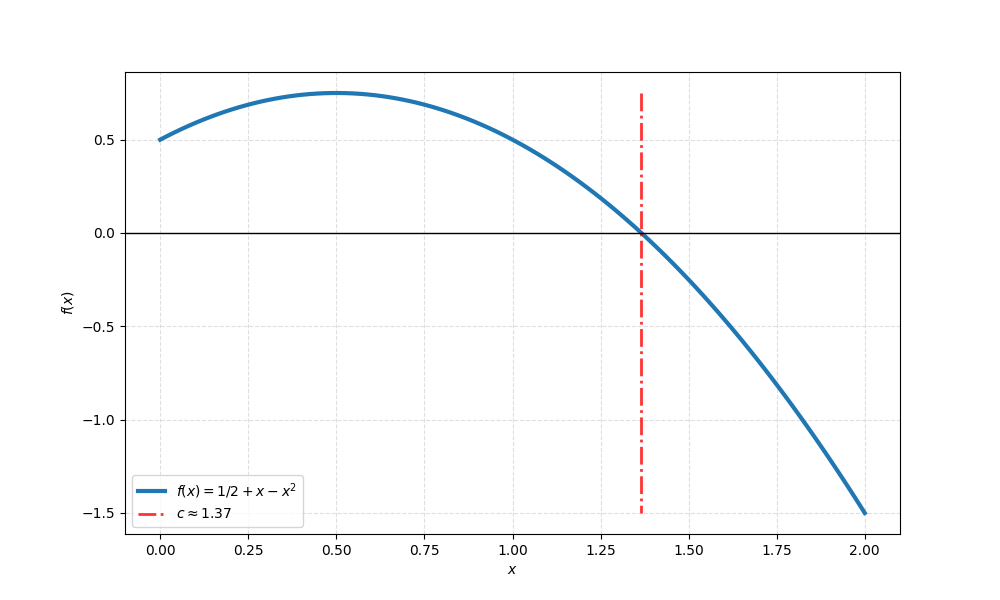
\includegraphics[width=0.8\linewidth]{images/12/plot_zero.png}
    \caption{Ricerca dello zero per $f(x)$}
    \label{fig: Zero bisec}
\end{figure}

\bigskip

\noindent Per quanto riguarda la convergenza di \textit{Bisection} e \textit{Regula Falsi}, accennavamo nel paragrafo precedente a come ci aspettiamo sia differente la velocità di convergenza alla soglia dei due algoritmi (sottolineando che però il rate rimane uguale per entrambi, essendo, sostanzialmente, lo stesso algoritmo con convergenza lineare): vogliamo in questa sezione mostrare questo comportamento con una rappresentazione dell'errore numerico e della distanza tra la \textit{guess} al passo n-esimo e il valore finale.

\medskip
\noindent Di seguito i grafici relativi ai due algoritmi: per ciascuno vediamo rappresentato sulla sinistra la convergenza della funzione, valutata nella \textit{guess}, allo zero matematico 
$$|f(c_n) - f(c_{true})| = |f(c_n) - 0| = |f(c_n)|$$
sulla destra troviamo la distanza n-esima della \textit{guess} da $c_{true}$, cioè l'errore al passo n-esimo
$$|c_n - c_{true}|=|c_n - \frac{1 + \sqrt{3}}{2}|$$

\medskip
\noindent La Fig. \ref{fig: Bis conv}, mostra il previsto andamento lineare di entrambi gli algoritmi: per quanto riguarda bisezione, l'andamento è caratterizzato da oscillazioni locali rispetto alla pendenza media. Al contrario, per Regula Falsi, si osserva come l'algoritmo mantenga l'ordine di convergenza  ma proceda in modo monotono: ogni iterazione riduce effettivamente la distanza dal valore vero. Nella bisezione, invece, la convergenza è garantita globalmente ma non è necessariamente decrescente passo dopo passo; può infatti accadere che:
$$\exists n \in [0, N_{max}] : |c_{n+1} - c| > |c_n - c|$$

\noindent Questa differenza riflette l'ottimizzazione introdotta dalla Regula Falsi: la scelta della \textit{guess} basata sull'interpolazione lineare risulta più efficace, specialmente su intervalli ridotti e per funzioni sufficientemente regolari. Il risultato è un processo di convergenza più "liscio" e rapido, pur restando nell'ambito della linearità.

\begin{figure}[H]
    \centering
    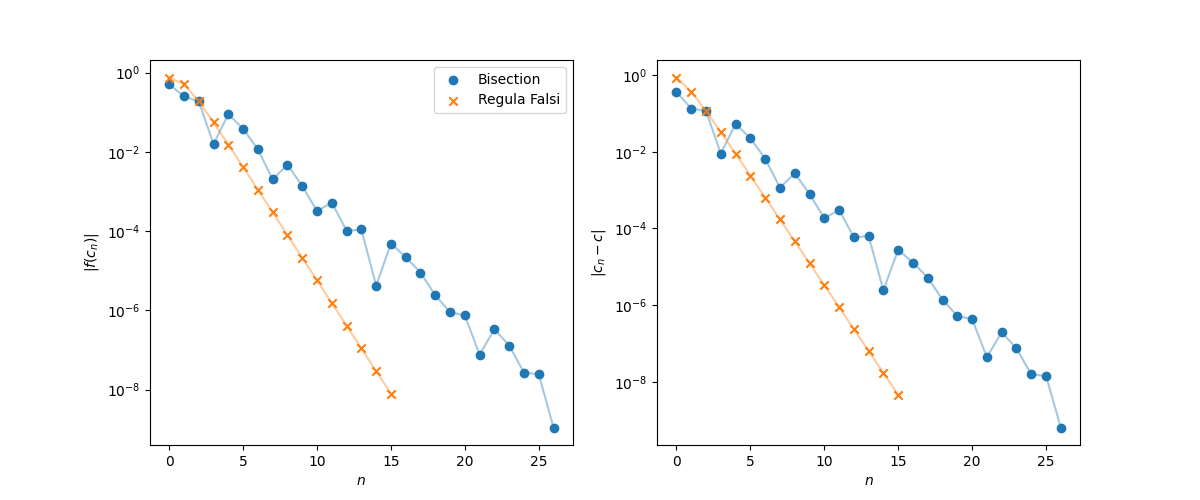
\includegraphics[width=\linewidth]{images/12/bis_vs_reg.png}
    \caption{Convergenza in funzione del numero di iterazioni dell'algoritmo di Bisezione e di Regula Falsi, per la funzione (sinistra) e il valore della radice (destra).}
    \label{fig: Bis conv}
\end{figure}

\noindent Con due fit dimostriamo, in Fig. \ref{fig: fit Bis} e Fig. \ref{fig: fit reg}, che l'andamento è lineare (fit su una retta di $\log(e_{k+1}) = \log(C) + p\log(e_k)$, con $p \approx 1$ per entrambe, dai risultati del fit). Da ora in avanti, quando ci si riferisce ai risultati di un fit per la convergenza di un algoritmo, valgono tutte le considerazioni che sono esplicitate e ampliate nell'Appendice (\hyperref[App: funzione fit]{App.1}) e sarà evitata la ripetizione delle stesse (vedi appunti sull'errore statistico dei risultati e setup del fit con forma logaritmica)

\begin{figure}[H]
    \centering
    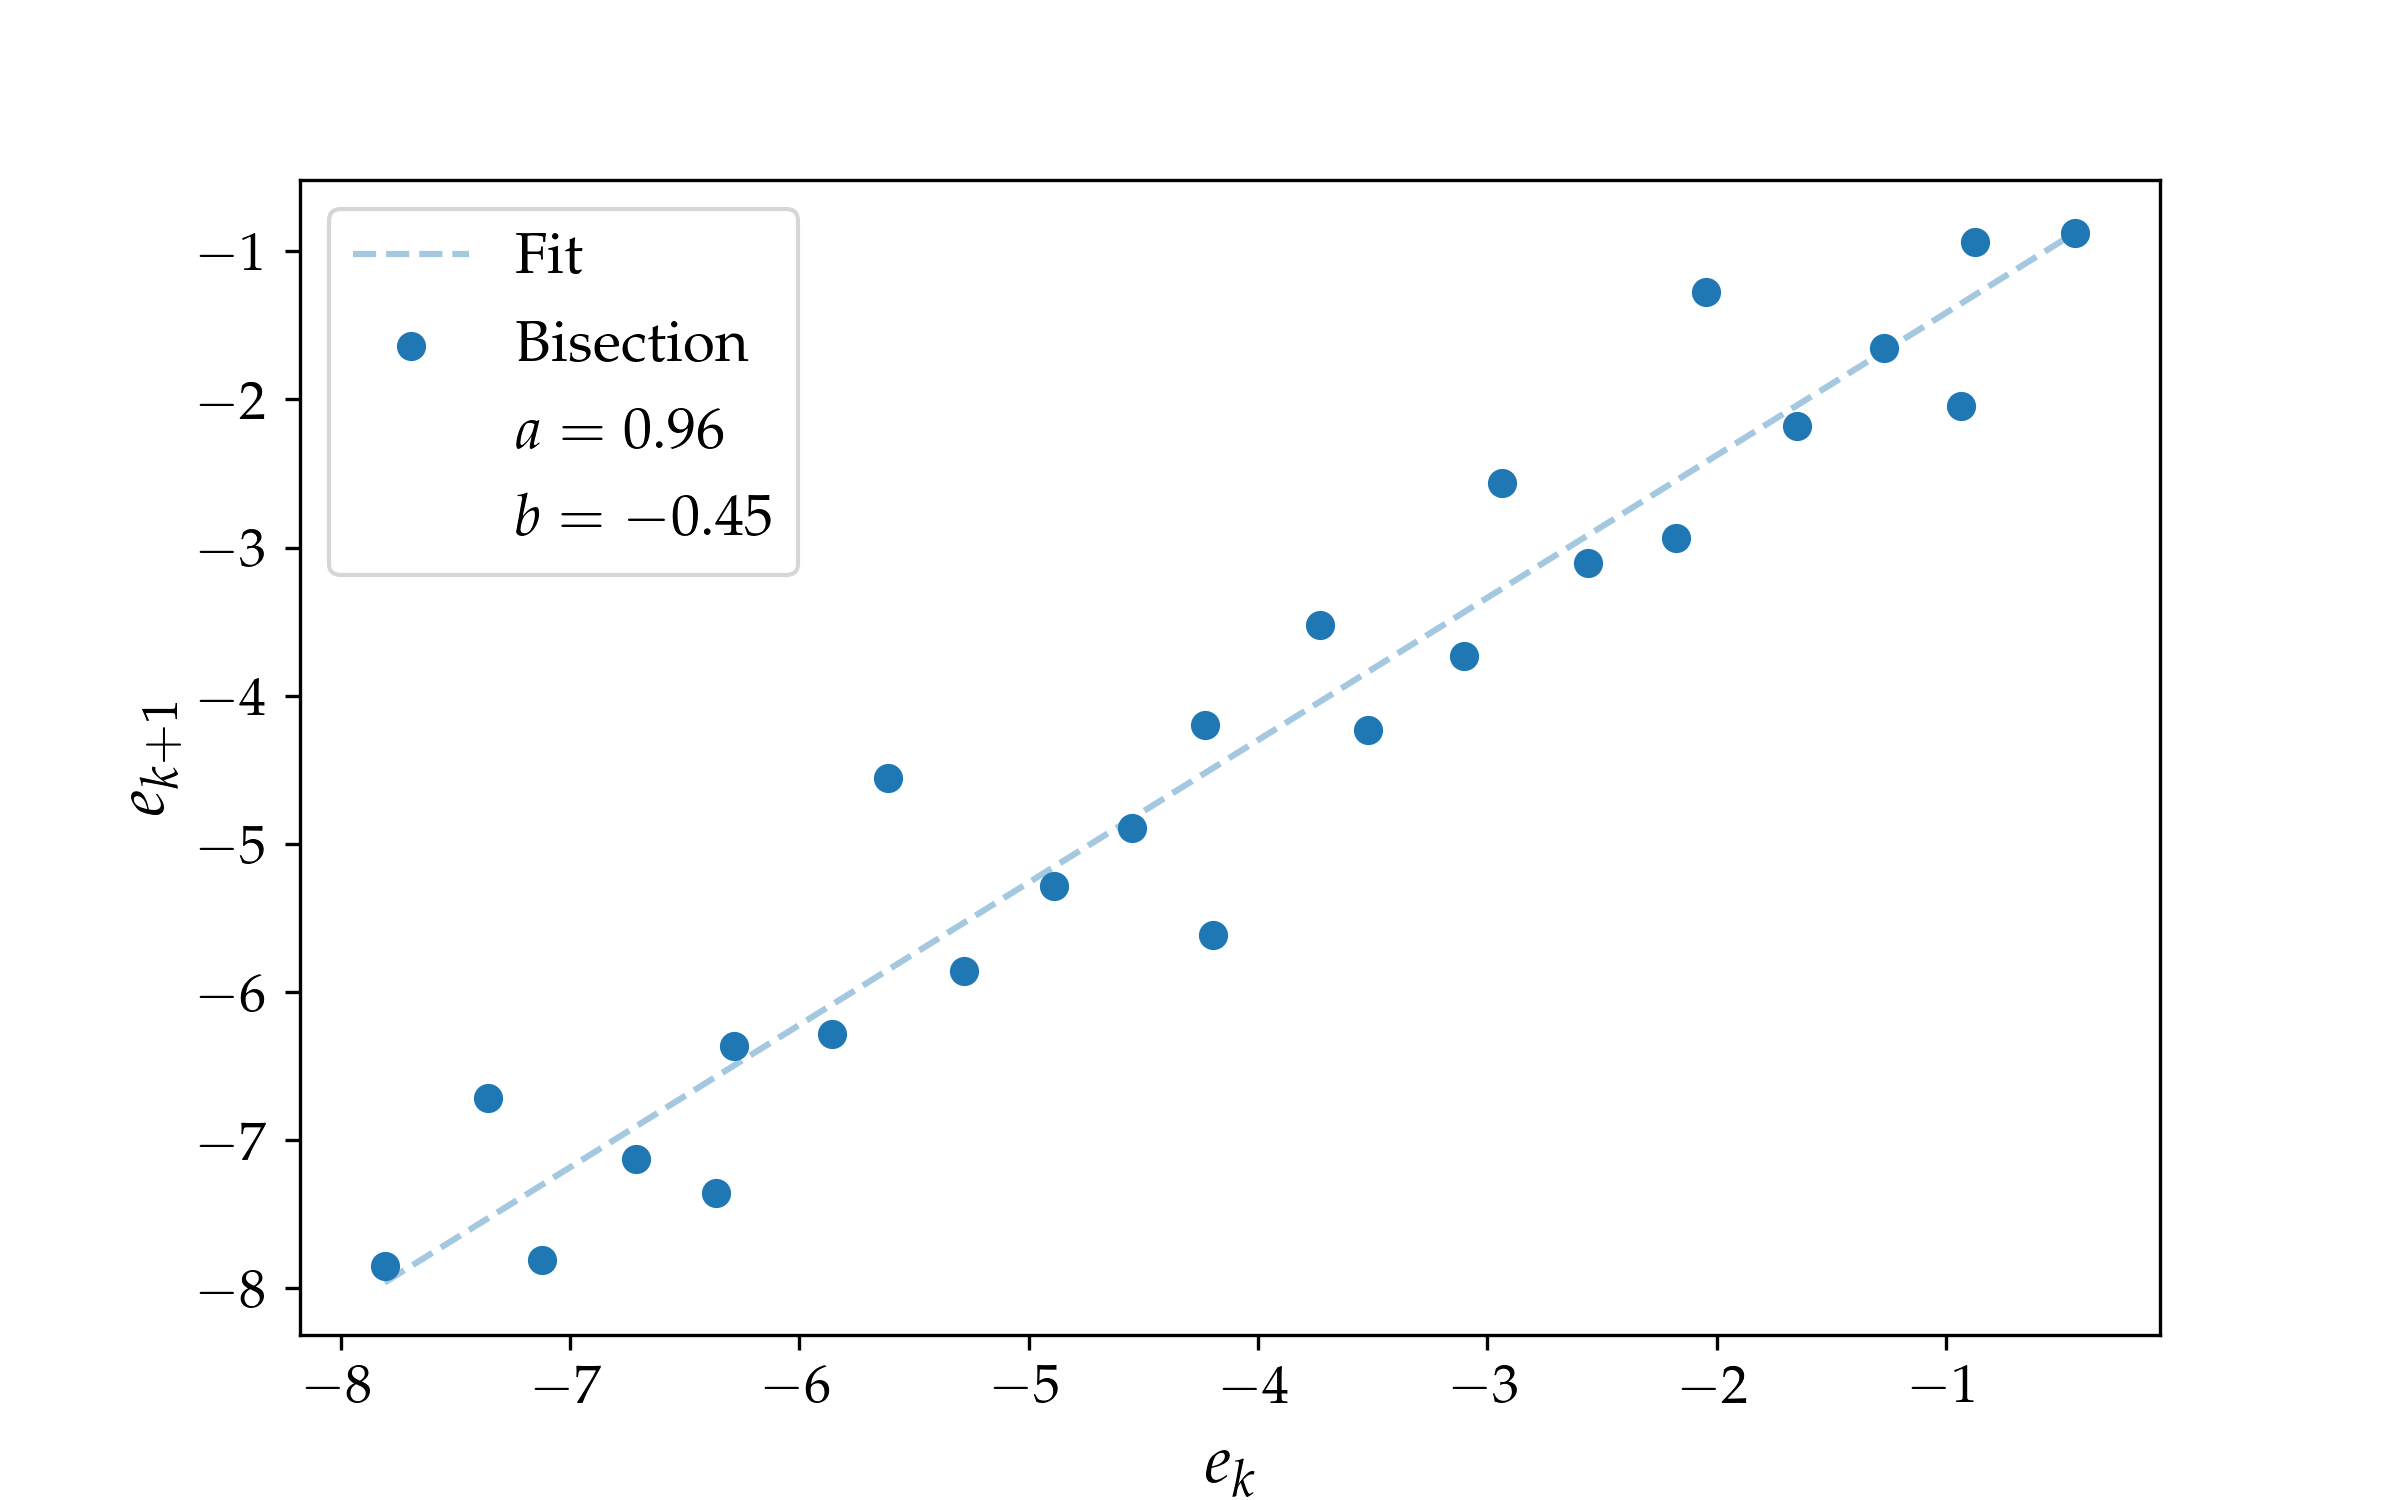
\includegraphics[width=0.8\linewidth]{images/12/fit_Bisection.png}
    \caption{Convergenza in funzione del numero di iterazioni dell'algoritmo di Bisezione. $e_k$, $e_{k+1}$ sono in realtà il $\log_{10}(e_i)$, abbreviato per semplicità con la formula senza il log: sull'asse sono indicate quindi le potenze del 10 a cui si riferiscono le grandezze.}
    \label{fig: fit Bis}
\end{figure}

\begin{figure}[H]
    \centering
    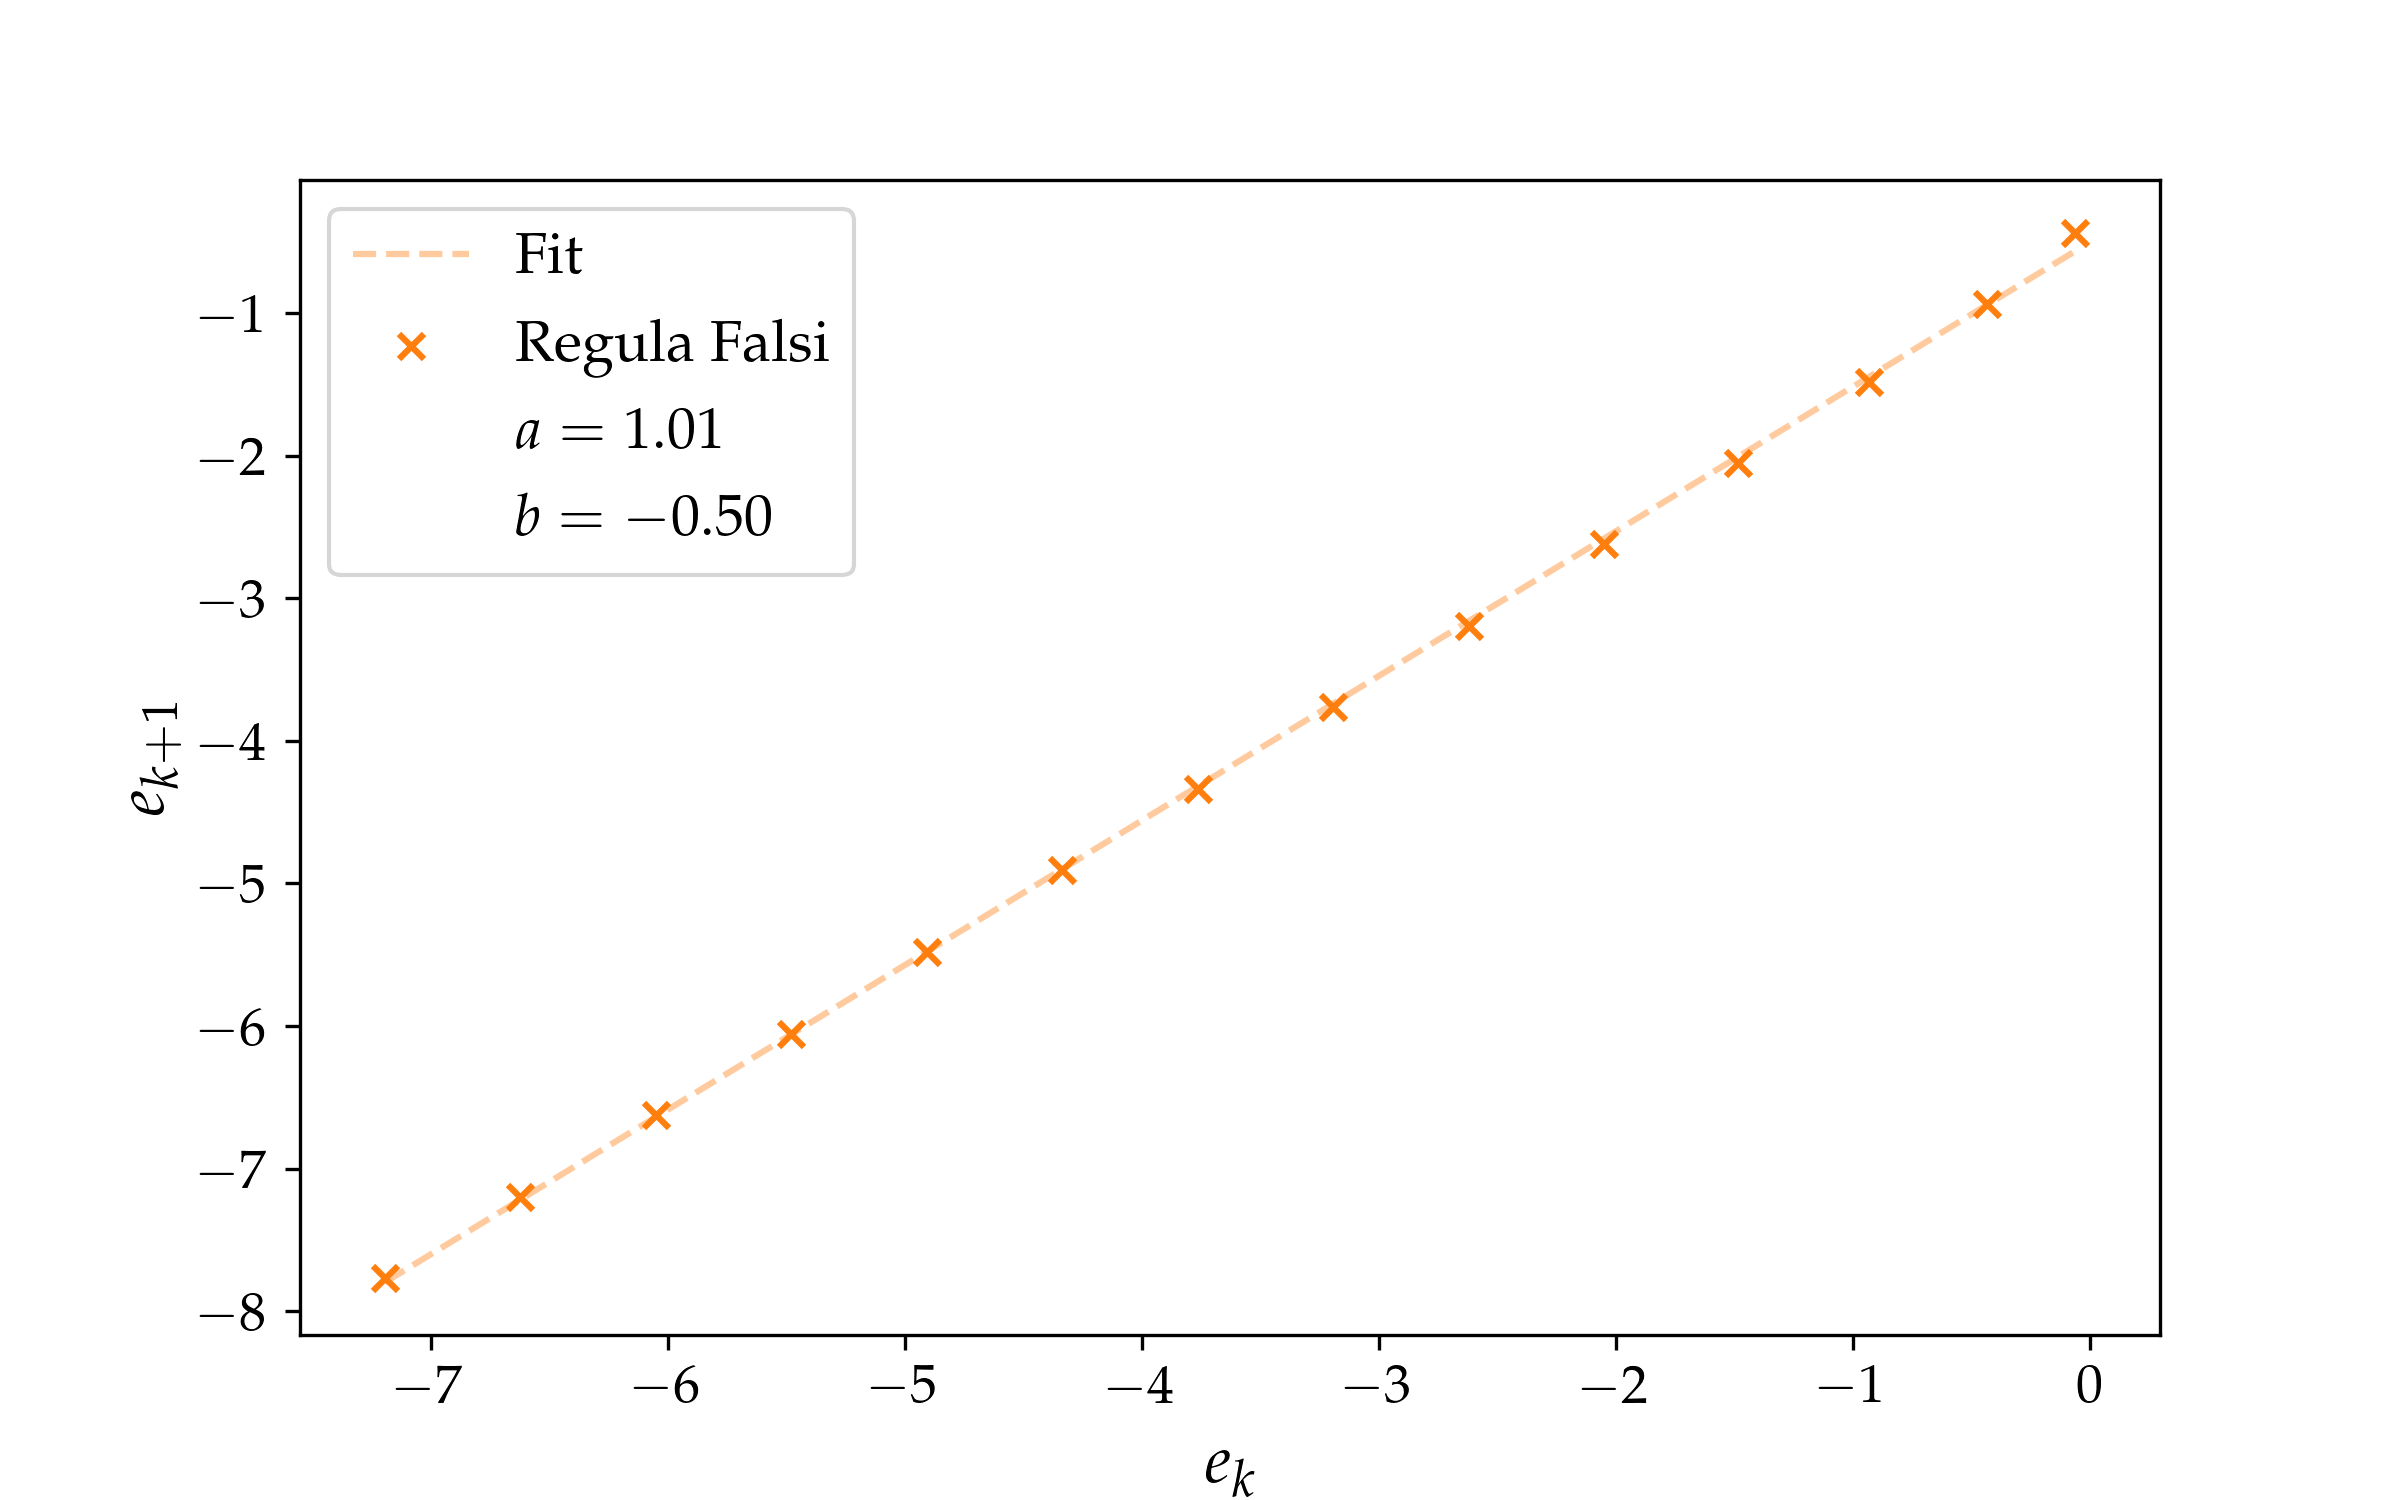
\includegraphics[width=0.8\linewidth]{images/12/fit_Regula_Falsi.png}
    \caption{Convergenza in funzione del numero di iterazioni dell'algoritmo di Regula Falsi. Per l'intestazione degli assi vale la stessa approssimazione del grafico sopra.}
    \label{fig: fit reg}
\end{figure}

\newpage










\section{Esercizio 5.1.2}
\subsection{Problem Statement}
Risolvi l'equazione di Keplero
\begin{equation} \label{eq: Keplero}
    M(t) = E(t) - e \sin(E(t))
\end{equation}

impostando i parametri $e = 0.5, a = 1$. Adotta la seguente regola per l'anomalia media $M(t) = 0.5t$.

\begin{enumerate}
    \item calcola il periodo $T$ da $E(T) = 2\pi$.
    \item prendi l'intervallo $t \in [0, T]$ e dividilo in 100 passi. Per ogni valore di $t$ calcola $E(t)$ trovando la radice dell'Eq. \ref{eq: Keplero} (usa il metodo della Regula Falsi) e le corrispondenti coordinate $x(t)$ e $y(t)$. Riporta i risultati in uno scatter plot.
    \item per un valore di $t$, studia la diversa convergenza in funzione del numero di iterazioni dei metodi della Regula Falsi e della bisezione.
\end{enumerate}

\subsection{Premessa Teorica}
Le \textit{Leggi di Keplero} descrivono le orbite ellittiche dei pianeti in rivoluzione attorno al sole. Rimanendo nel piano bidimensionale, esse sono definite come segue:

\begin{equation*} \label{eq: Kep Law}
    \begin{array}{ll}
    x(t) = a (\cos E(t)- e) \\
    y(t) = a \sqrt{1-e^2} \sin (E(t))
    \end{array}
\end{equation*}

\noindent dove introduciamo $0<e<1$, eccentricità dell'orbita e $E(t)$, anomalia eccentrica. Quest'ultima è legata dall'Eq. \ref{eq: Keplero} a $M(t)$, che definiamo anomalia media. 

\subsection{Metodi Numerici e Algoritmi}
Ci viene fornita la forma funzionale per $M(t) = 0.5t$: ciò permette di ricercare il valore di $E(t)$ per via numerica, semplicemente leggendo Eq. \ref{eq: Keplero} come
\begin{equation} \label{eq: root research}
M(t) - E(t) + e \sin(E(t)) = 0
\end{equation}

\noindent cioè trovando la radice di questa funzione $f(E(t))=0$. Due metodi di \textit{root finder} sono già stati implementati in Cap. \ref{sec. bisec e Regula Falsi} e saremo interessati al confronto dei loro risultati.

\bigskip
\noindent In primis troviamo il periodo dell'orbita, cercando $T$ in $E(T) = 2 \pi$:
\[
M(T) = 0.5T = E(T) - e  \sin(E(T)) = 2\pi
\]
\[
\implies T = 4 \pi
\]

\noindent Campionando l'intervallo $[0, T]$ con 100 valori valutiamo gli zeri t-esimi di Eq. \ref{eq: root research} (scegliamo di utilizzare il metodo \textit{Regula Falsi}), trovando $E(t)$ e risolvendo poi le \textit{Leggi di Keplero} per la determinazione delle coordinate $x(t), y(t)$.


\subsection{Risultati e Discussione}
La valutazione delle posizioni $x, y$ permette di disegnare l'orbita su un piano 2D: questa rappresentazione porta con sè anche alcune altre informazioni sulla dinamica del pianeta, per esempio dalla distanza dei marker possiamo visualizzare la velocità tangenziale del corpo
\footnote{
Le parti in cui la densità dei marker aumenta sono quelle in cui la velocità è minore, sapendo che i fotogrammi sono equispaziati nello span temporale. Possiamo notare come ciò avvenga nell'intorno della zona di massima curvatura. Si può osservare che per le parti con velocità maggiore vale il viceversa (e sarà interessata la zona speculare dell'orbita).}
. Nella Fig. \ref{fig: color_orbit} desideriamo mostrare proprio questo andamento, con un plot che, utilizzando una mappa di colore, rappresenta l'istante temporale a cui è riferita la posizione dello \textit{scatter plot}, cioè la posizione del pianeta sull'orbita in funzione del tempo.\\
Disegniamo una stella nella posizione di uno dei due fuochi ($x=y=0$): è semplice osservare che la velocità è massima nel punto di \textit{Perielio}, cioè quando la distanza tra il pianeta e la stella è minima, viceversa la velocità è minima per il punto di \textit{Afelio}, dove la distanza è massima.\\
La conferma e spiegazione di ciò è data dalla \textit{Seconda Legge di Keplero}, che afferma:
\begin{quote}
    ``Il segmento (raggio vettore) che unisce il centro del Sole con il centro del pianeta descrive aree uguali in tempi uguali.'' 
\end{quote}
È naturale concludere con le affermazioni che abbiamo enunciato a proposito della relazione tra massime e minime velocità e posizioni relative del pianeta nella sua orbita.\\
In particolare l'animazione "\textit{ani\_kep.mp4}", disponibile al link Github repo \url{https://github.com/mvolpato-unimib/Lab_comp/tree/main/ex12/plots}, 
è una chiara esemplificazione di ciò: ho unito nel plot la dinamica del pianeta sulla sua orbita e la rappresentazione dell'area spazzata dal raggio vettore in uno span di 30 istanti, mostrando che l'area rimane conservata e che la velocità cambia come abbiamo descritto precedentemente. 

\begin{figure}[H]
    \centering
    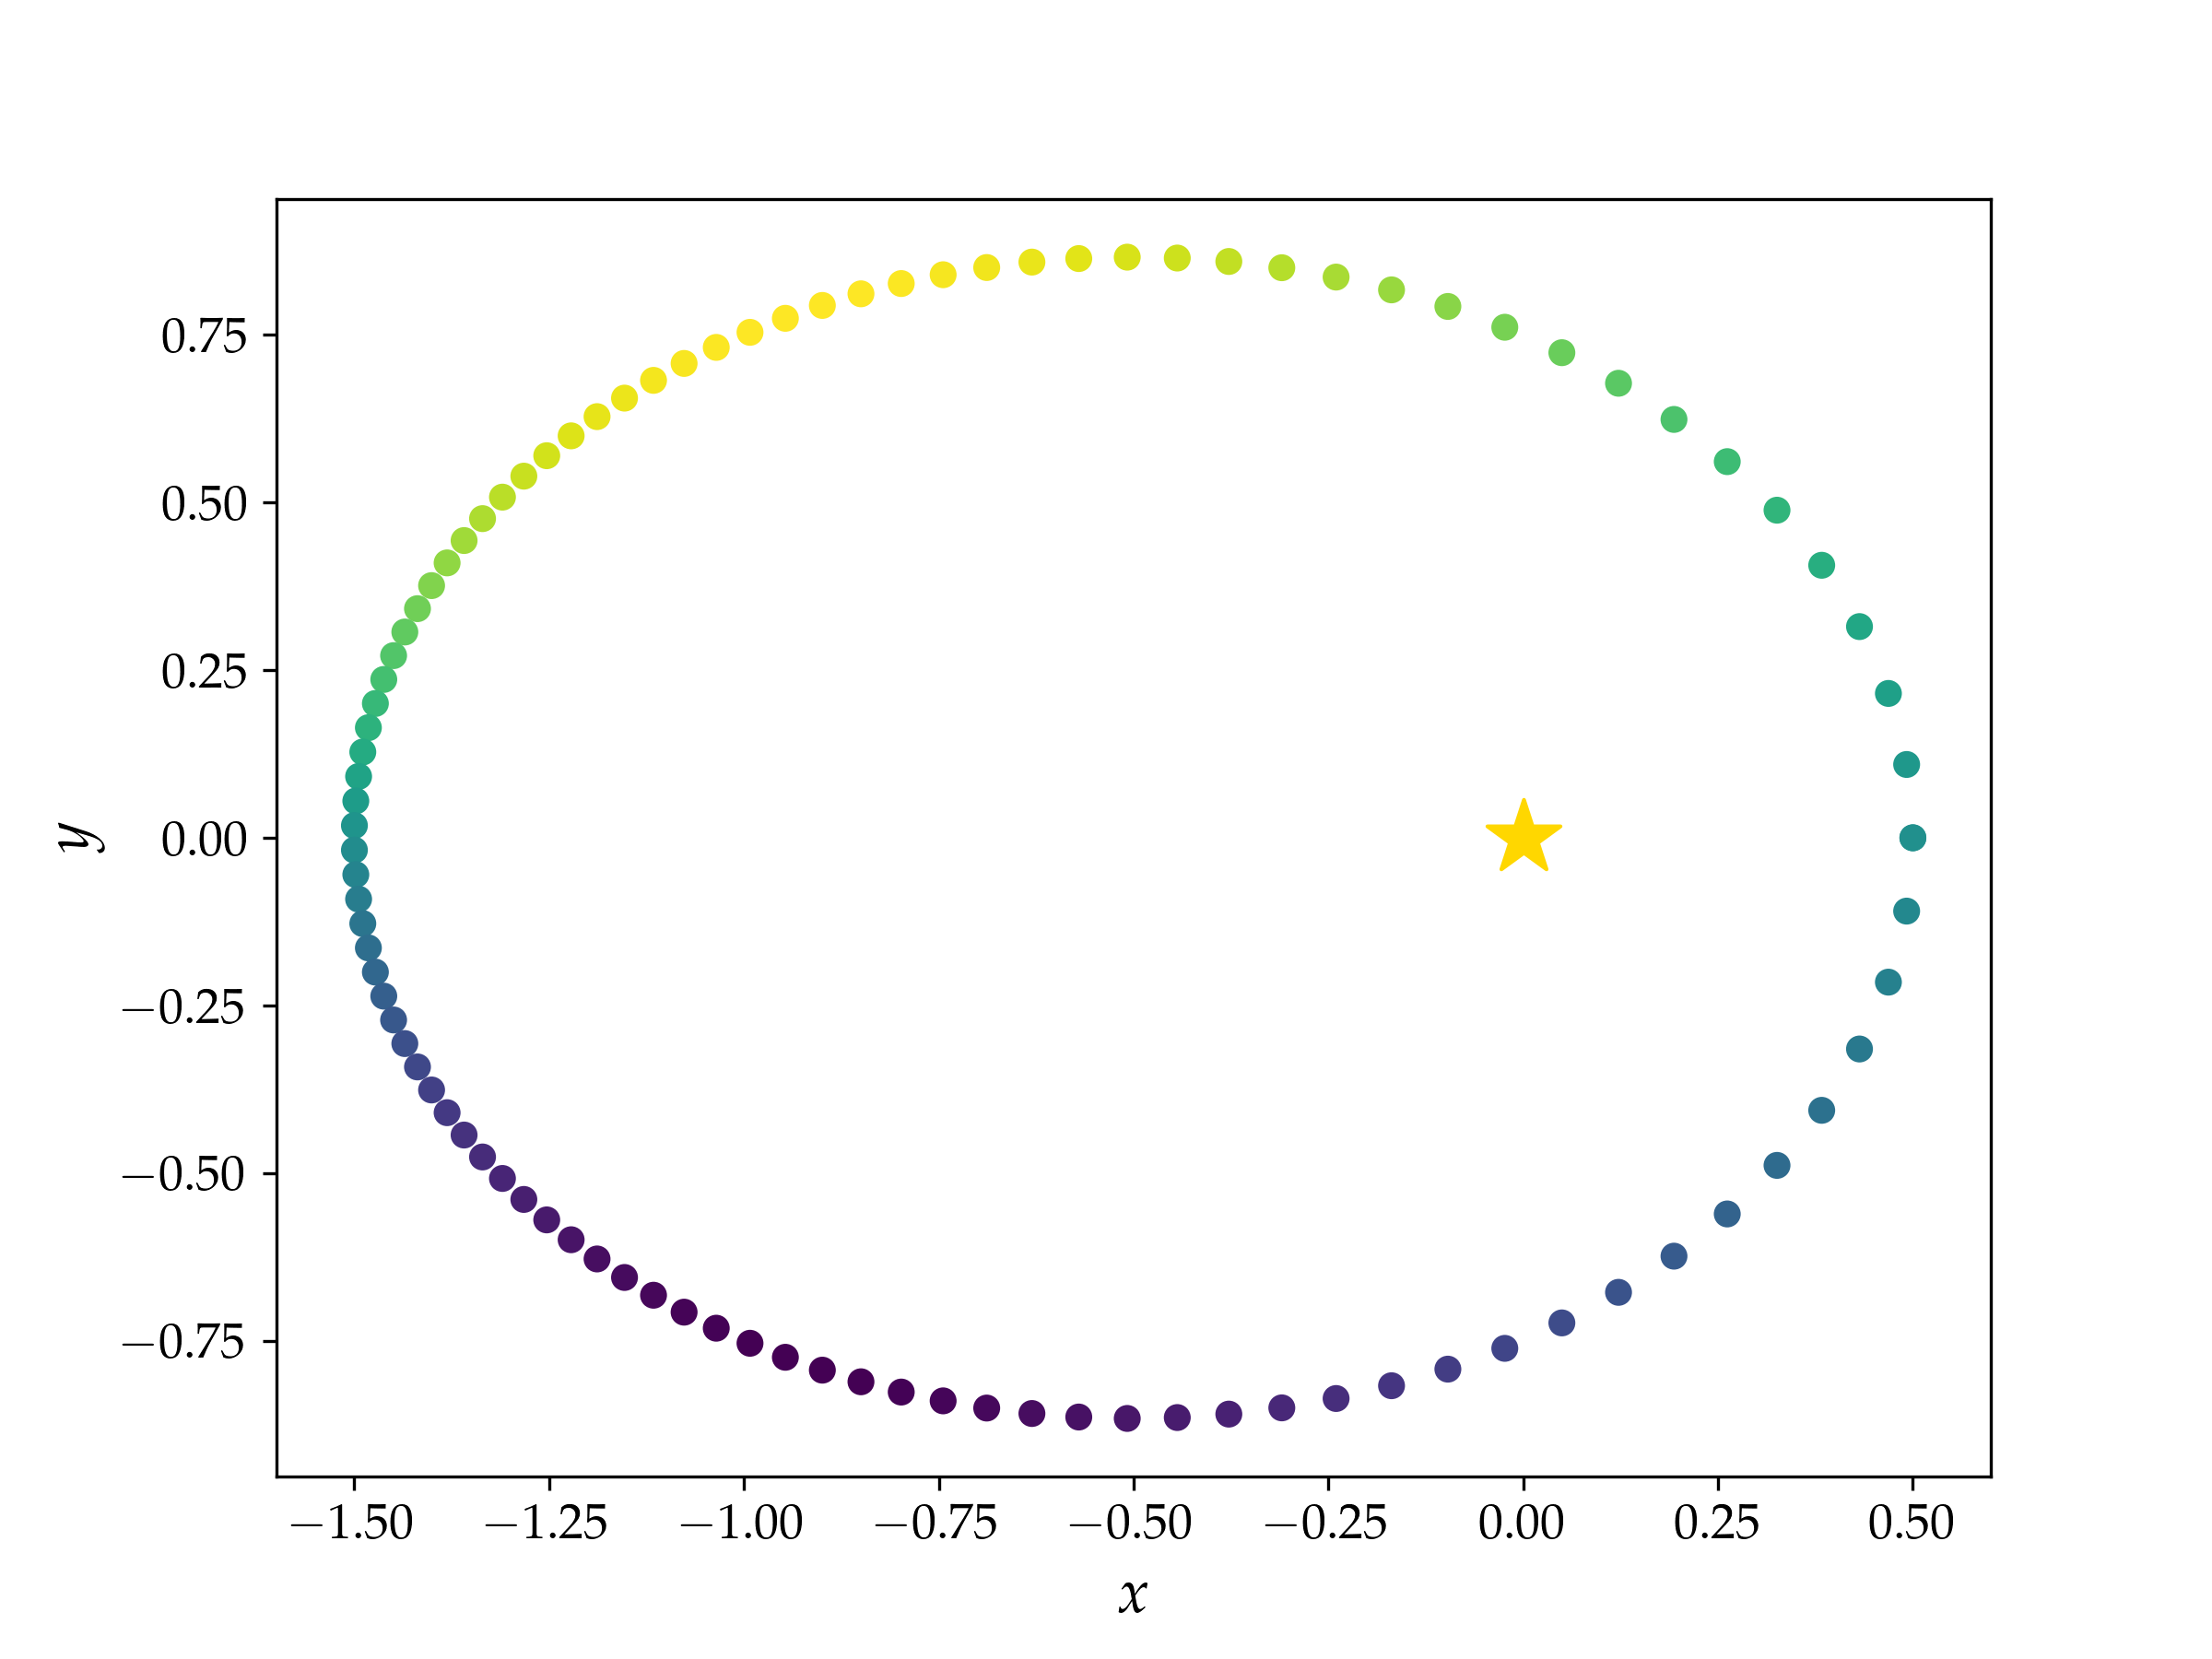
\includegraphics[width=0.8\linewidth]{images/12/color_orbit.png}
    \caption{Orbita del pianeta attorno al fuoco (stella). La mappa di colore indica l'istante temporale, da cui dipende la posizione del corpo.}
    \label{fig: color_orbit}
\end{figure}

\noindent Infine desideriamo confrontare come l'algoritmo di ricerca delle radici, in questo caso di default \textit{Regula Falsi}, abbia diversa convergenza in base al metodo. La discussione sarà del tutto simile a quella del Cap. \ref{sec: risultati bisec regula}, dove analizzavamo Fig. \ref{fig: Bis conv}. Rimettiamo al riferimento a quella sezione le specifiche dei plot, ma concludiamo che vengono confermate tutte le considerazioni precedenti: entrambi i metodi hanno convergenza lineare, ma con costanti di convergenza differenti, il che si riflette in un numero di iterazioni significativamente diverso.

\medskip
\noindent Fissato un valore di $t\in [0, T]$, scegliamo $t=1$, possiamo effettuare la ricerca della radice della funzione
\[
f(E(1)) = 0.5  - E(1) + e \cdot \sin(E(1)) = 0
\]
scegliamo un intervallo $I=[-1, 5]$, tale che $f(-1)\cdot f(5) < 0$ (per assicurare la presenza della radice), che servirà anche per inizializzare i due algoritmi. Plottiamo in Fig. \ref{fig: zero Kep} l'andamento della funzione nell'intervallo. 

\begin{figure}[H]
    \centering
    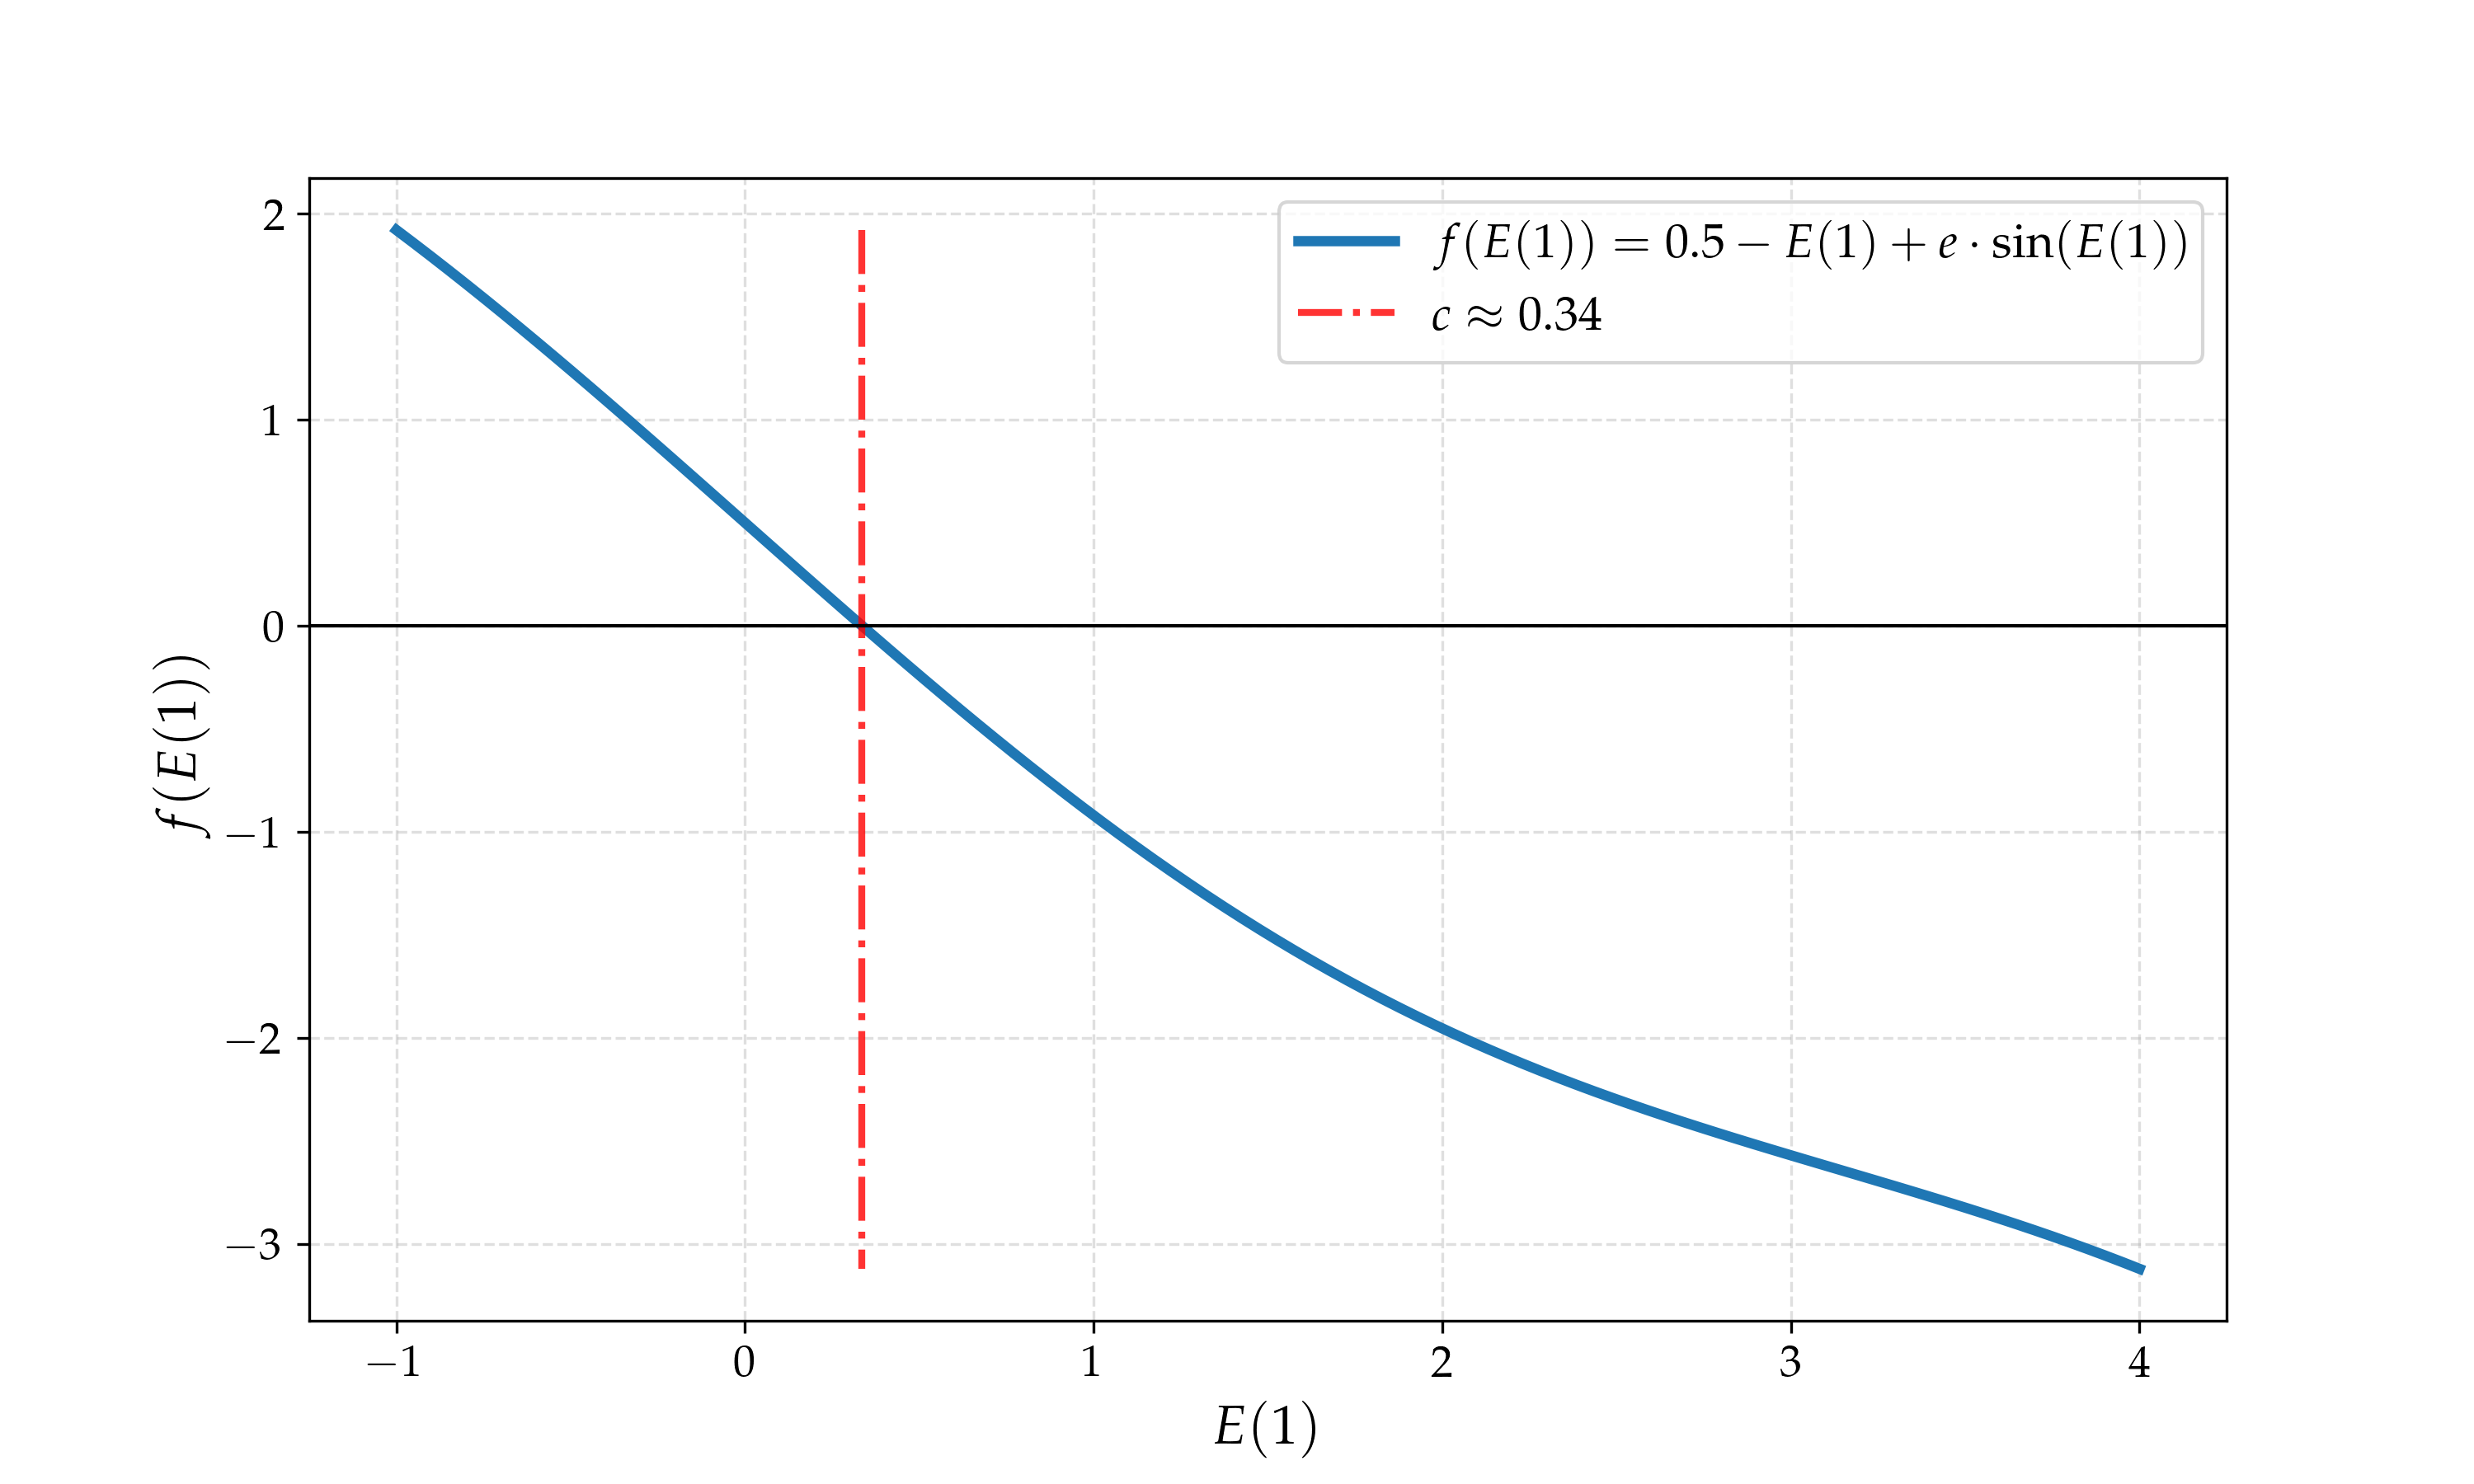
\includegraphics[width=0.8\linewidth]{images/12/plot_Kep_zero.png}
    \caption{Ricerca dello zero per $f(E(1))$.}
    \label{fig: zero Kep}
\end{figure}

Gli algoritmi restituiscono questi risultati:

\begin{elegantcode}
- BISECTION MTH
     Found f(c) = 0:  c =  0.3354180343449116
     N_iter =  29

- REGULA FALSI
     Found f(c) = 0:  c =  0.33541803238804735
     N_iter =  5

diff = 1.956864226215771e-09
\end{elegantcode}

\noindent Infine in Fig. \ref{fig: conv kep} la convergenza rispettivamente della funzione e dell'errore sulla radice e il controllo dell'ordine (aspettato lineare e verificato, $a\approx1$) con un fit sui dati del caso di bisezione (Fig. \ref{fig: kep fit bis}).

\medskip
\noindent
Si noti che se dai risultati del metodo si può leggere che il numero di iterazioni è stato di $n_{iter}=5$ per Regula Falsi, i punti sui grafici sono quattro; questo perché il confronto per valutare l'errore viene fatto sull'ultimo punto valutato, preso di riferimento come valore vero: di conseguenza $n \in [0, N_{iter}-1]$.\\

\medskip \noindent
Manca il grafico relativo al fit dell'algoritmo di Regula Falsi, poiché il confronto $e_k$ vs $e_{k+1}$ riduce i punti: inizialmente abbiamo $e_k = (e_1, \dots, e_{n-1})$, decidendo di non considerare l'ultimo elemento, costruiamo $e_{k+1} = (e_2, \dots, e_{n-1})$, abbiamo così definito una coppia di vettori che confrontati rappresentano le coppie di errori ad un passo $k$ e $k+1$.\\
Nel caso specifico, con $N_{iter} = 4$, abbiamo: 
\begin{align*}
e_k &= (e_1, \dots, e_{n-2}), \\
e_{k+1} &= (e_2, \dots, e_{n-1}) \\
&\xrightarrow{\text{ }} e_k = (e_1, e_2), \\
&\xrightarrow{\text{ }} e_{k+1} = (e_2, e_3)
\end{align*}

\noindent Si ottiene un fit con solo due punti, non significativo per una analisi dell'andamento da studiare: non è quindi stato incluso alcun grafico per il fit di questo secondo metodo.

\begin{figure} [H]
    \centering
    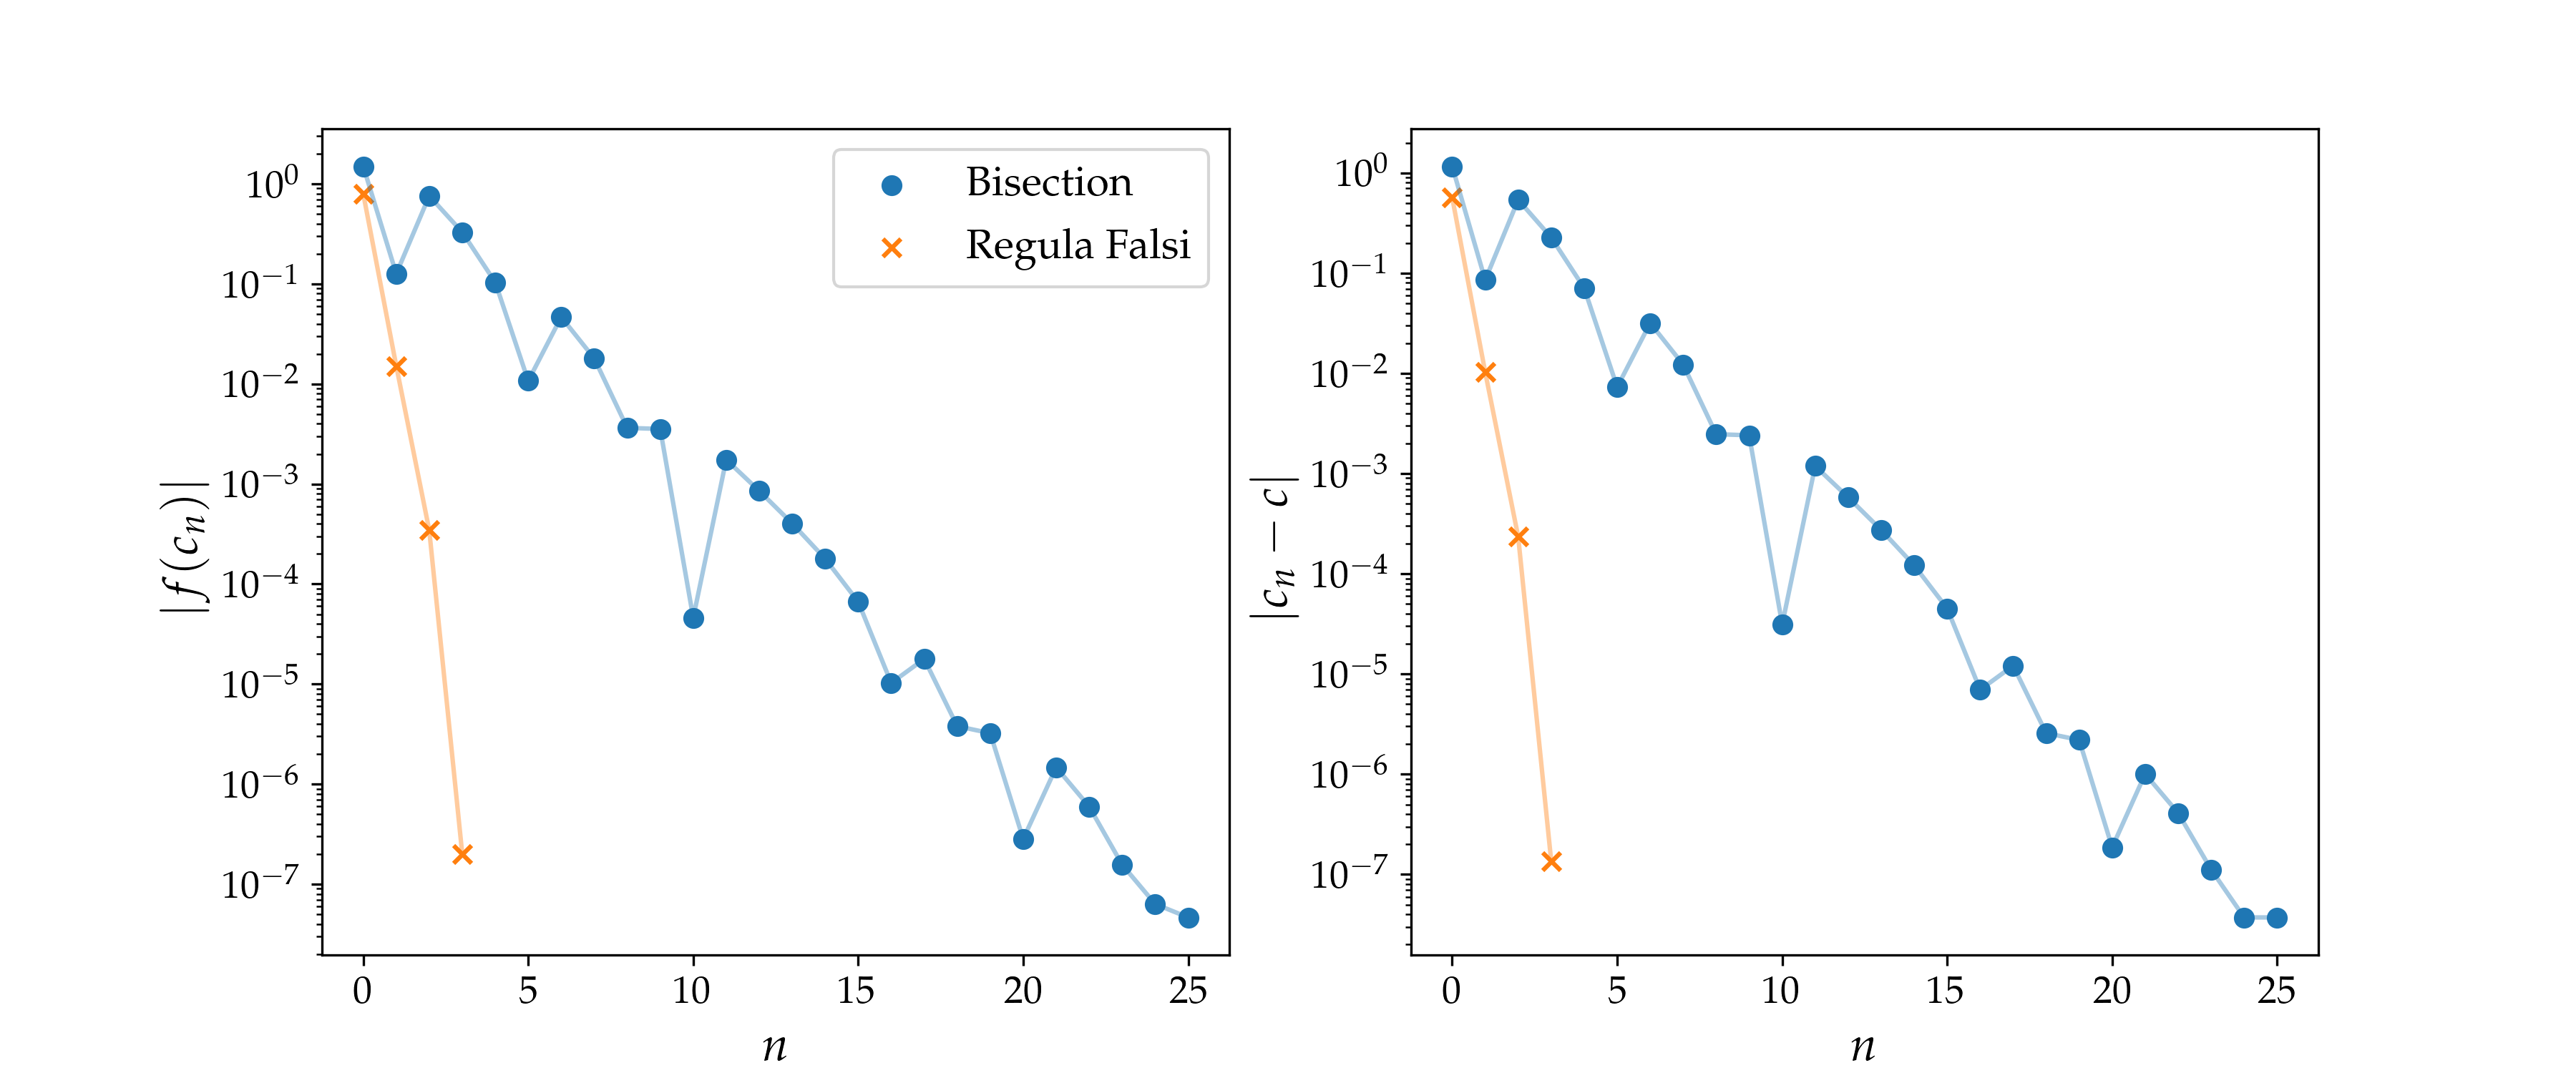
\includegraphics[width=\linewidth]{images/12/bis_vs_reg_keplero.png}
    \caption{Confronto della convergenza in funzione del numero di iterazioni dell'algoritmo di Bisezione vs Regula Falsi  per la funzione (sinistra) e il valore della radice (destra).}
    \label{fig: conv kep}
\end{figure}

\begin{figure} [H]
    \centering
    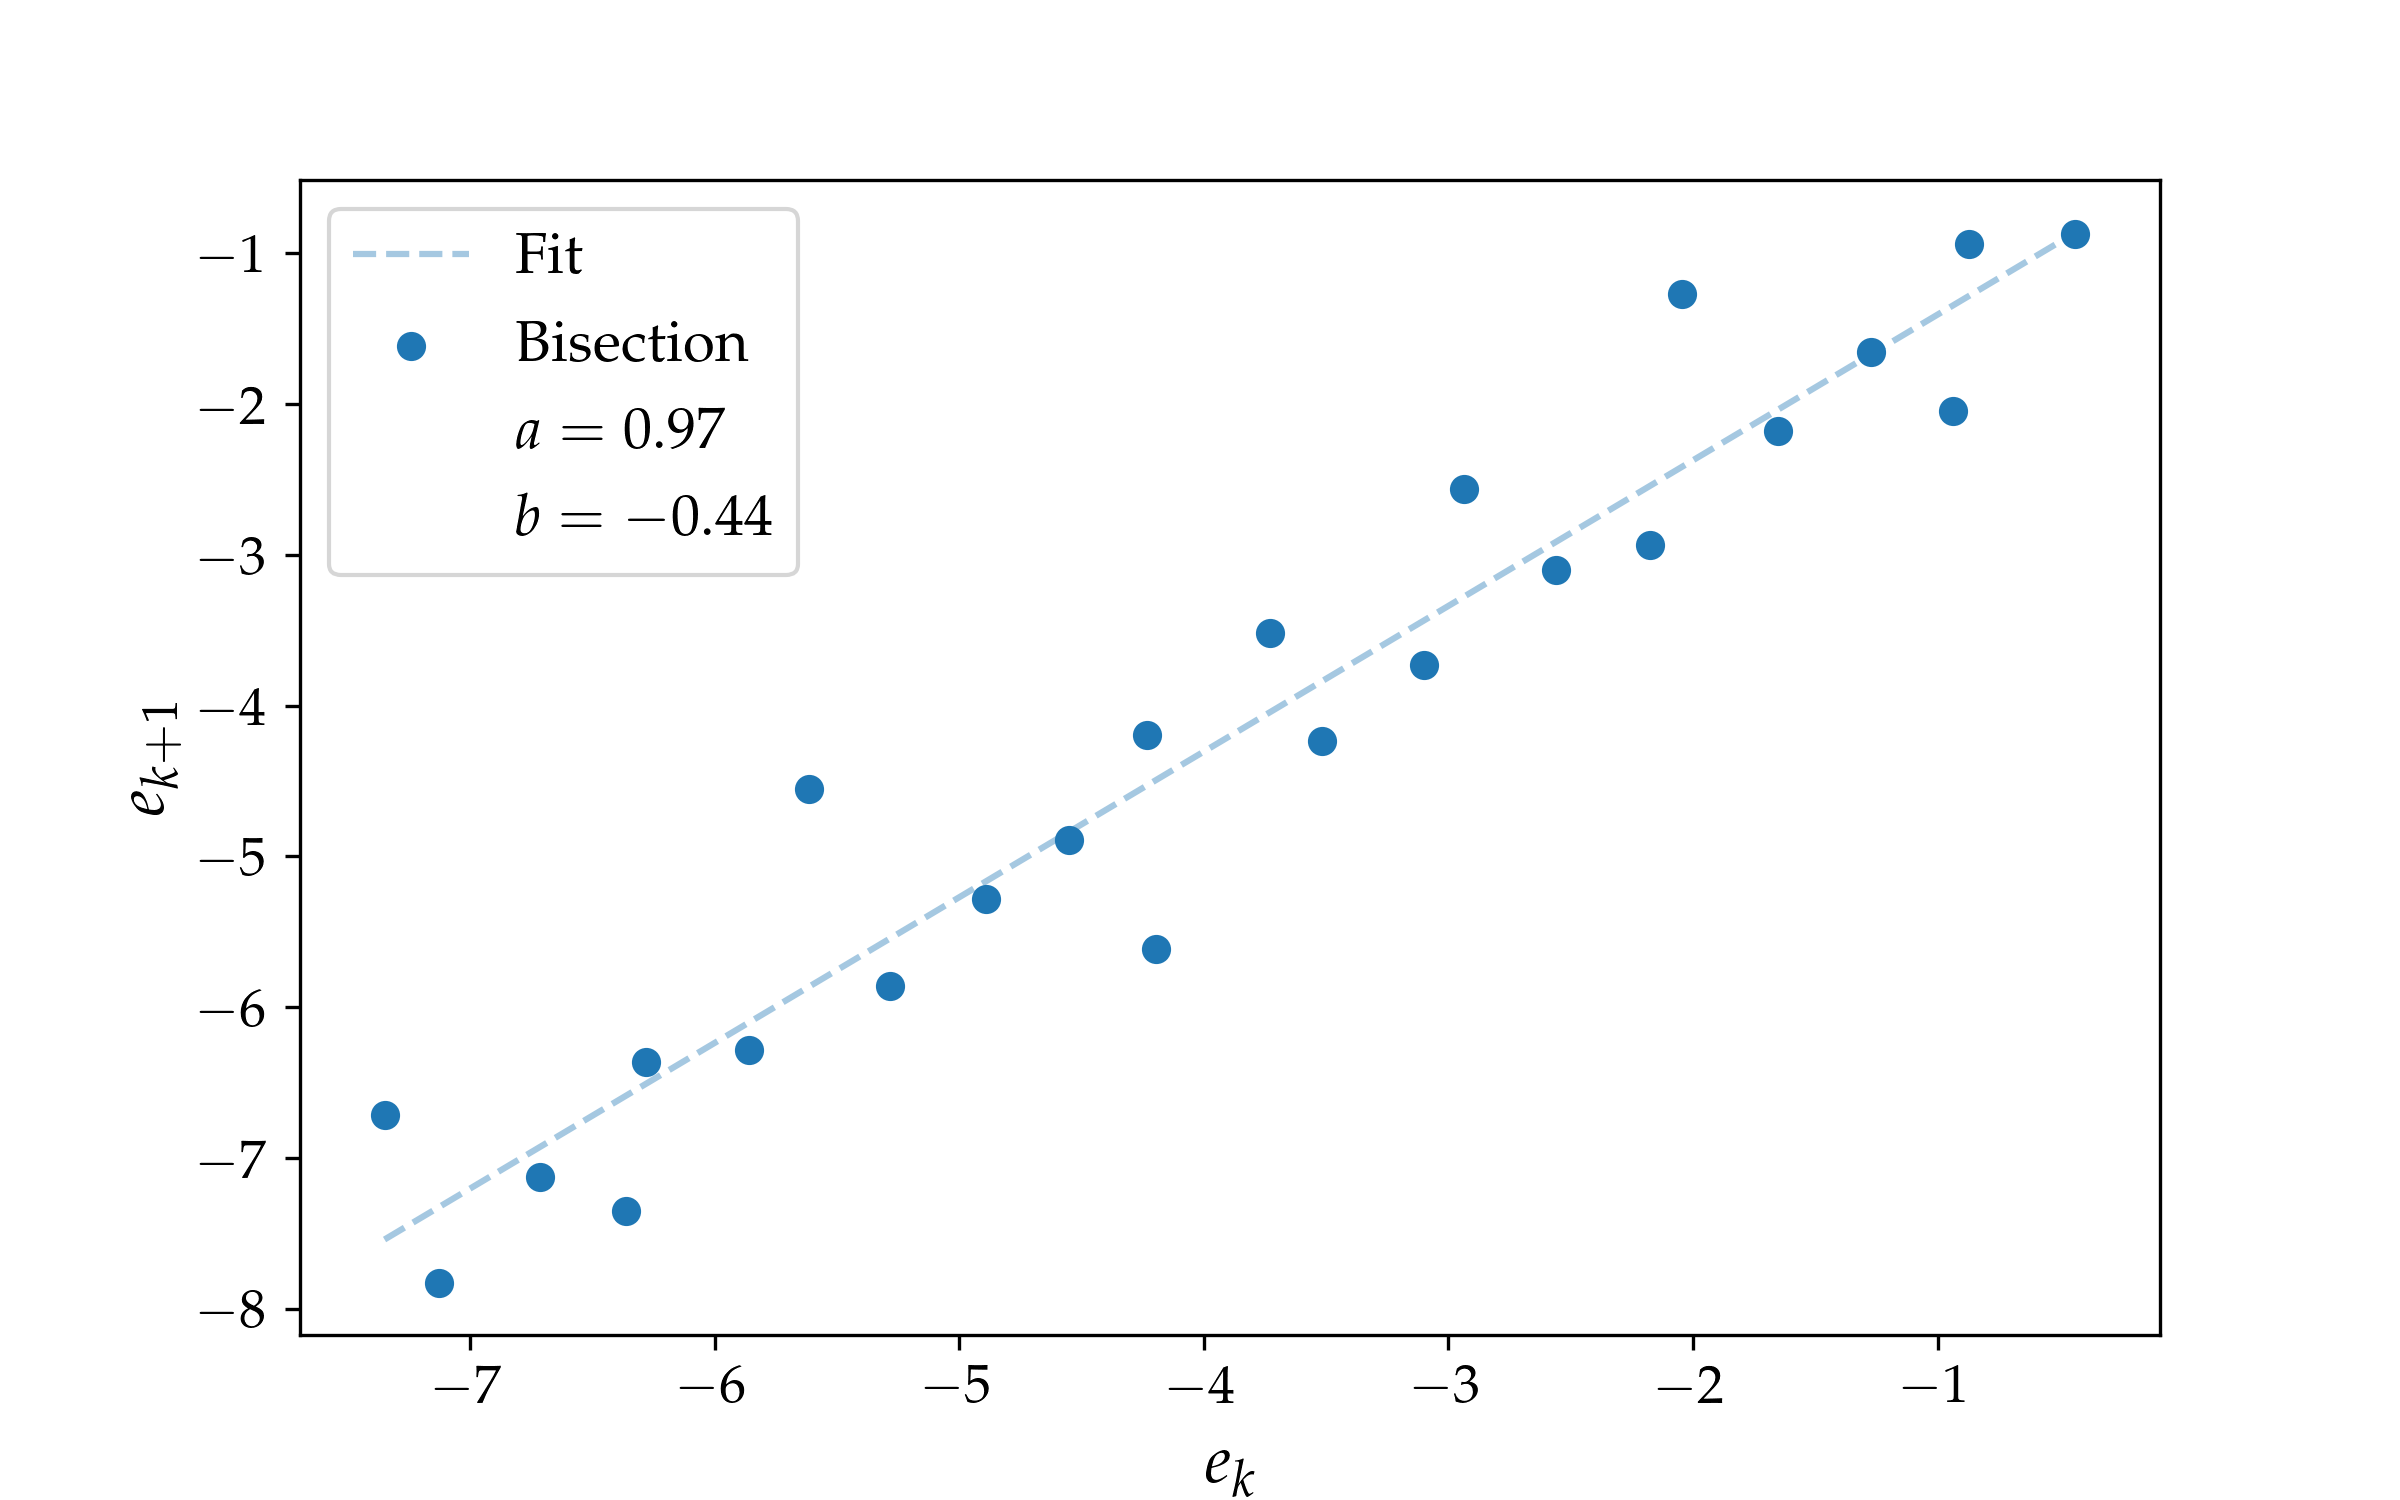
\includegraphics[width=0.8\linewidth]{images/12/keplero_fit_Bisection.png}
    \caption{Convergenza in funzione del numero di iterazioni dell'algoritmo di Bisezione. Per l'intestazione degli assi vale la stessa approssimazione di Fig. \ref{fig: fit Bis}.}
    \label{fig: kep fit bis}
\end{figure}

\newpage






\section{Esercizio 5.2.1}

\subsection{Problem Statement}
Scrivete una funzione che implementi l'algoritmo di Newton e studiate i tre casi seguenti, che dovrebbero illustrare i problemi di questo metodo.

\subsection*{1. Convergenza lenta}
Considerate la funzione $f(x) = x^2$ e calcolate la sua radice con l'algoritmo di Newton-Raphson, partendo da $x_0 = 0.8$. La convergenza è quadratica? Spiegatelo utilizzando sia evidenze analitiche che quelle numeriche.

\subsection*{2. Cicli}
In alcuni casi il metodo di Newton non converge mai poiché, a causa di una commissione tra la funzione e l'ipotesi iniziale, l'algoritmo entra in un ciclo infinito. Considerate la funzione $f(x) = x^3 - 2x + 2$ e le ipotesi iniziali $x_0 = 0$ e $x_0 = 1$. Tracciate i valori della radice $x_n$ in funzione di $n$. Perché oscilla tra 0 e 1? Una volta compreso il meccanismo, trovate una soluzione.

\subsection*{3. Condizioni iniziali}
L'algoritmo di Newton può essere molto suscettibile alle condizioni iniziali, in particolare se scegliamo un'ipotesi iniziale (o se finiamo per trovarci su un punto) in cui la derivata prima è molto vicina a zero. Ciò può portare a un grande salto in una singola iterazione, che manda l'algoritmo in una regione più vicina a una soluzione diversa rispetto a quella che stavamo affrontando.

\medskip

Per illustrare il problema della forte sensibilità alle condizioni iniziali, immaginiamo di dividere un certo dominio in un insieme discreto di punti, applicare l'algoritmo di Newton a ciascun punto per una data funzione che ammette almeno 2 radici e poi vedere a quale radice converge ciascun punto. Successivamente, possiamo assegnare un colore a ogni soluzione e mappare la sensibilità alle condizioni iniziali sotto forma di confini tra aree di colori diversi.

Consideriamo i numeri complessi e prendiamo la funzione

$$f(z) = (z^2 - 1)(z^2 + 1)$$

con quattro radici $1, -1, i, -i$. Per assegnare un colore a ogni radice, calcolate semplicemente l'angolo in coordinate polari della soluzione corrispondente.

Successivamente, create una griglia di punti nel piano complesso bidimensionale, dove la densità della griglia specifica il numero di \textit{pixel} che abbiamo.



\subsection{Premessa Teorica}
Abbiamo già presentato due esempi di algoritmi che sono definiti \textit{bracketed}, cioè per cui l'inizializzazione del metodo è legata alla definizione di un intervallo in cui assicuriamo la convergenza. Questo punto di forza è bilanciato dall'ordine di convergenza, lineare, che limita il loro utilizzo. \\
L'algoritmo di Newton-Raphson offre un'altra possibilità: ci permette di migliorare la convergenza rispetto al \textit{metodo di bisezione} (o \textit{Regula Falsi}) passando ad uno scaling quadratico; paghiamo sulla robustezza del metodo, che non assicura più la convergenza, dato un certo punto $x_0$ con cui inizializzare. 

\subsection{Metodi Numerici e Algoritmi}
Il metodo di N-R è definito come segue:\\
data la funzione $f$ e supponendo esista una sua radice $L$ nel nostro dominio di ricerca ($f(L)=0$), è possibile definire l'algoritmo iterativo di \textit{Newton-Raphson} (N-R) 
\[
    x_{n+1} \equiv x_n - \frac{f(x_n)}{f'(x_n)}
\]

\noindent Da questa definizione si può dimostrare che l'errore al passo n-esimo è dato da:
\[
    L - x_{n+1} = - \frac12 \frac{f''(L)}{f'(x_n)} (L-x_n)^2 + O((x_n-L)^3)
\]
cioè per una radice semplice ($f'(L) \not=0$) il metodo di Newton presenta convergenza quadratica. 
\medskip

\noindent Le problematiche di questo metodo sono legate al ruolo che giocano la derivata prima e seconda all'interno delle relazioni: il loro rapporto può accelerare o rallentare fortemente l'algoritmo e in particolare un valore di $f'(x) \approx 0$ potrebbe causare la non convergenza (questo termine si trova al denominatore in entrambe le equazioni). Il vantaggio di aumentare la potenza di scaling è compensato dal pericolo di far fallire l'algoritmo lavorando con delle condizioni iniziali sconvenienti. 



\subsection{Risultati e Discussione}
\subsubsection{Convergenza lenta}
Seguendo la consegna, inizializziamo l'algoritmo con $x_0=0.8$, la funzione di test è $f(x)=x^2$:\\
la valutazione analitica della radice è $L=0$, notando che $f(L), f'(L)=0$. Ci aspettiamo di vedere un cambiamento nel fattore di scaling, come avevamo proposto nel paragrafo precedente e con alcuni passaggi analitici è possibile dimostrare ciò in forma generale.

\medskip
\noindent
Ripartendo con la definizione dell'algoritmo in forma iterativa:
\[
    x_{n+1} \equiv x_n - \frac{f(x_n)}{f'(x_n)}
\]
sviluppiamo $f(x_n), f'(x_n)$ con Taylor per $x_n = L$, cioè intorno alla nostra radice:
\begin{align*}
    f(x_n) &= f(L) + x_n f'(L) + \frac{x_n^2}{2}f''(L) + O(x_n^3)\\
    f'(x_n) &= f'(L) + x_n f''(L) + O(x_n^2)
\end{align*}
ricordando $f(L), f'(L)=0$:
\begin{align*}
    f(x_n) &= \frac{x_n^2}{2}f''(L) + O(x_n^3) = x_n^2 (\frac{1}{2} f''(L) + O(x_n))\\
    f'(x_n) &=x_n f''(L) + O(x_n^2) = x_n (f''(L) + O(x_n))
\end{align*}

\begin{align*}
\xrightarrow{}  x_{n+1} &=  x_n - \frac{x_n^2 (\frac{1}{2}f''(L) + O(x_n))}{x_n (f''(L) + O(x_n))} \\
&\approx  x_n - x_n \frac{\frac{1}{2}f''(L)}{f''(L)} \\
&\approx  x_n (1 - 1/2) 
\end{align*}

\[
x_{n+1} \approx\frac{1}{2} x_n
\]

risultato valido in forma generale per $f(L), f'(L)=0$: nel nostro caso:

\[
L=0 \implies x_i = |L-x_i| = e_i 
\]

La relazione finale, espressa in termini dell'errore al passo $n$:
\begin{align*}
\implies e_{n+1} &\approx\frac{1}{2} e_n \\
\implies \log_{10}(e_{n+1}) &\approx \log_{10}(e_n) + \log_{10}(1/2)  \\
\end{align*}

\noindent In particolare di seguito nella forma utilizzata per il fit e una stima dei parametri attesi con questa derivazione analitica: 
\begin{align*}
\implies \epsilon_{n+1} &\approx a\cdot \epsilon_{n} + b\ \\
\epsilon_i =\log_{10}(e_i),\ a&=1,\ b =  \log_{10}(1/2) \approx -0.3
\end{align*}

\noindent Ciò che vogliamo confermare con questo esempio è che il metodo, con le appropriate condizioni iniziali, può modificare il suo \textit{scaling}, non riproducendo un carattere quadratico, ma, come è reso evidente in questo caso, un andamento lineare nell'ordine di convergenza.\\

\medskip\noindent
In Fig. \ref{fig: N-R lin repr} una rappresentazione delle radici trovate sulla funzione di test al variare del numero di interazioni, in Fig. \ref{fig: fit NR lin} il fit della funzione, dove si noti che i parametri stimati numericamente coincidono con i risultati analitici.

\begin{figure}[H]
    \centering
    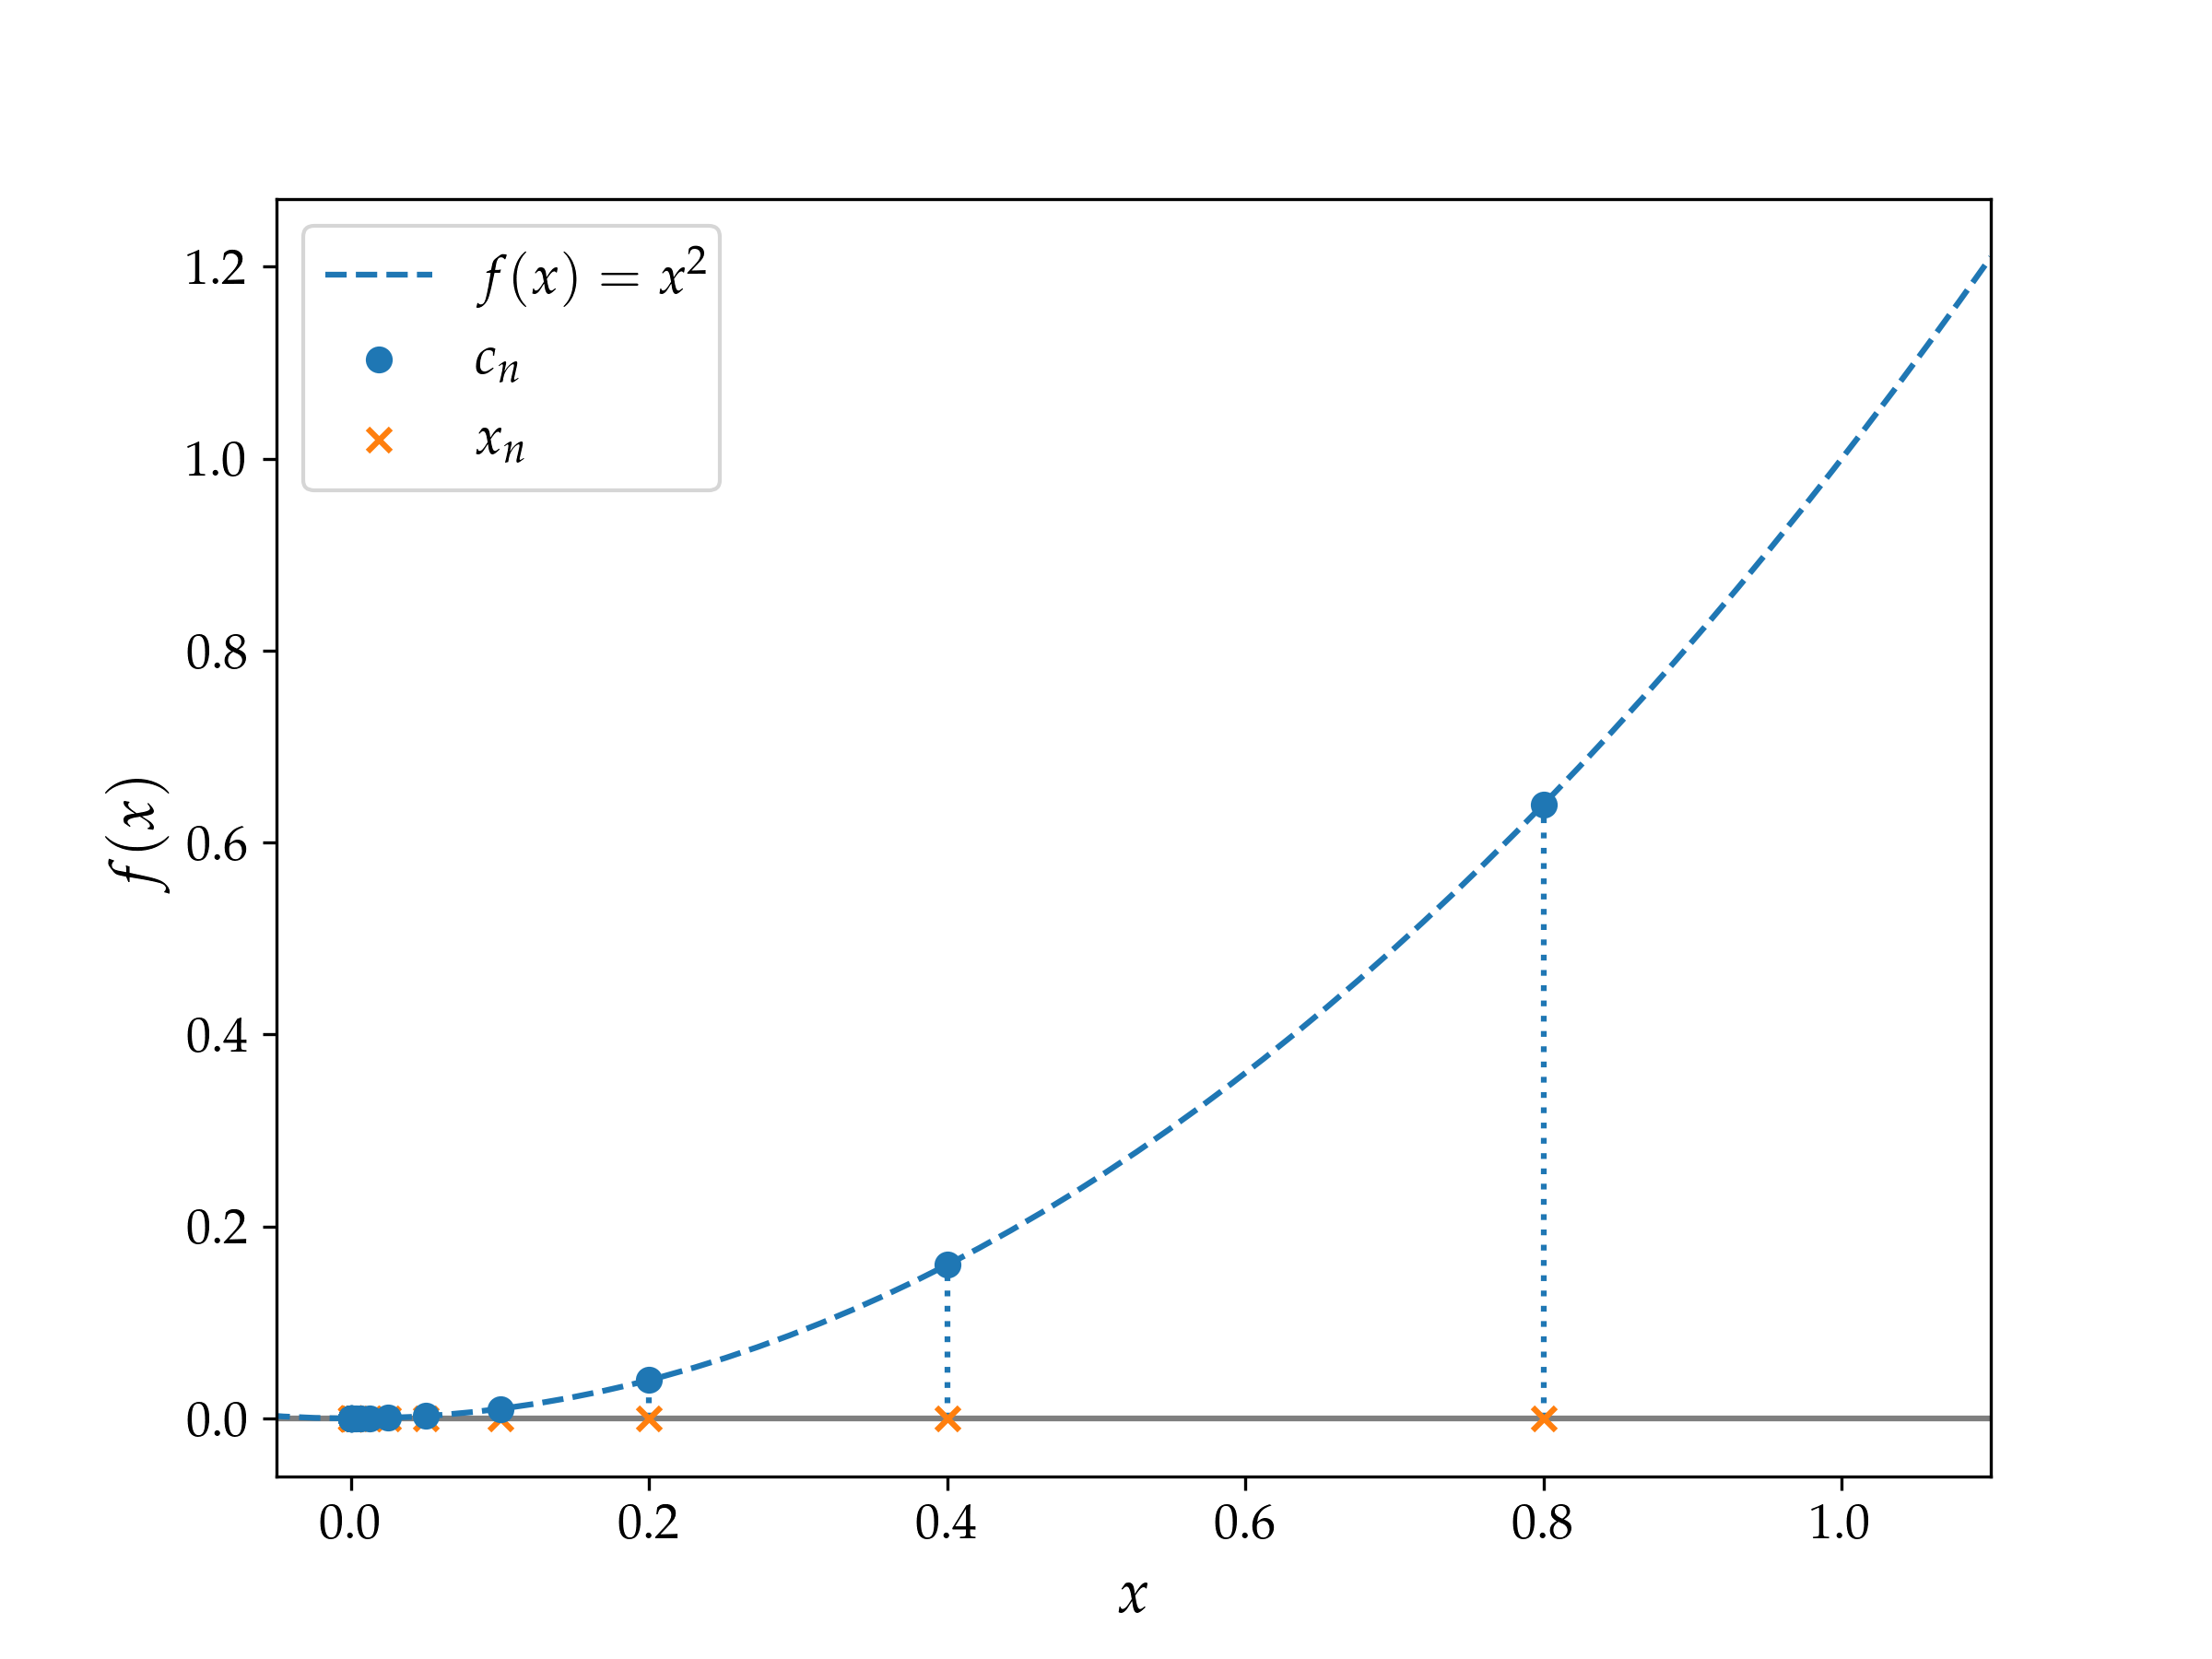
\includegraphics[width=0.7\linewidth]{images/13/init_cond.png}
    
    \caption{I risultati dell'algoritmo N-R con la funzione $f(x)= x^2\ ,\ x_0=0.8$: $x_n$ rappresentano le radici al passo n-esimo, dove si può osservare la convergenza al valore analitico di $x=0$, i $c_n$ sono invece i punti $(x_n, f(x_n)).$}
    \label{fig: N-R lin repr}
\end{figure}

\begin{figure}[H]
    \centering
    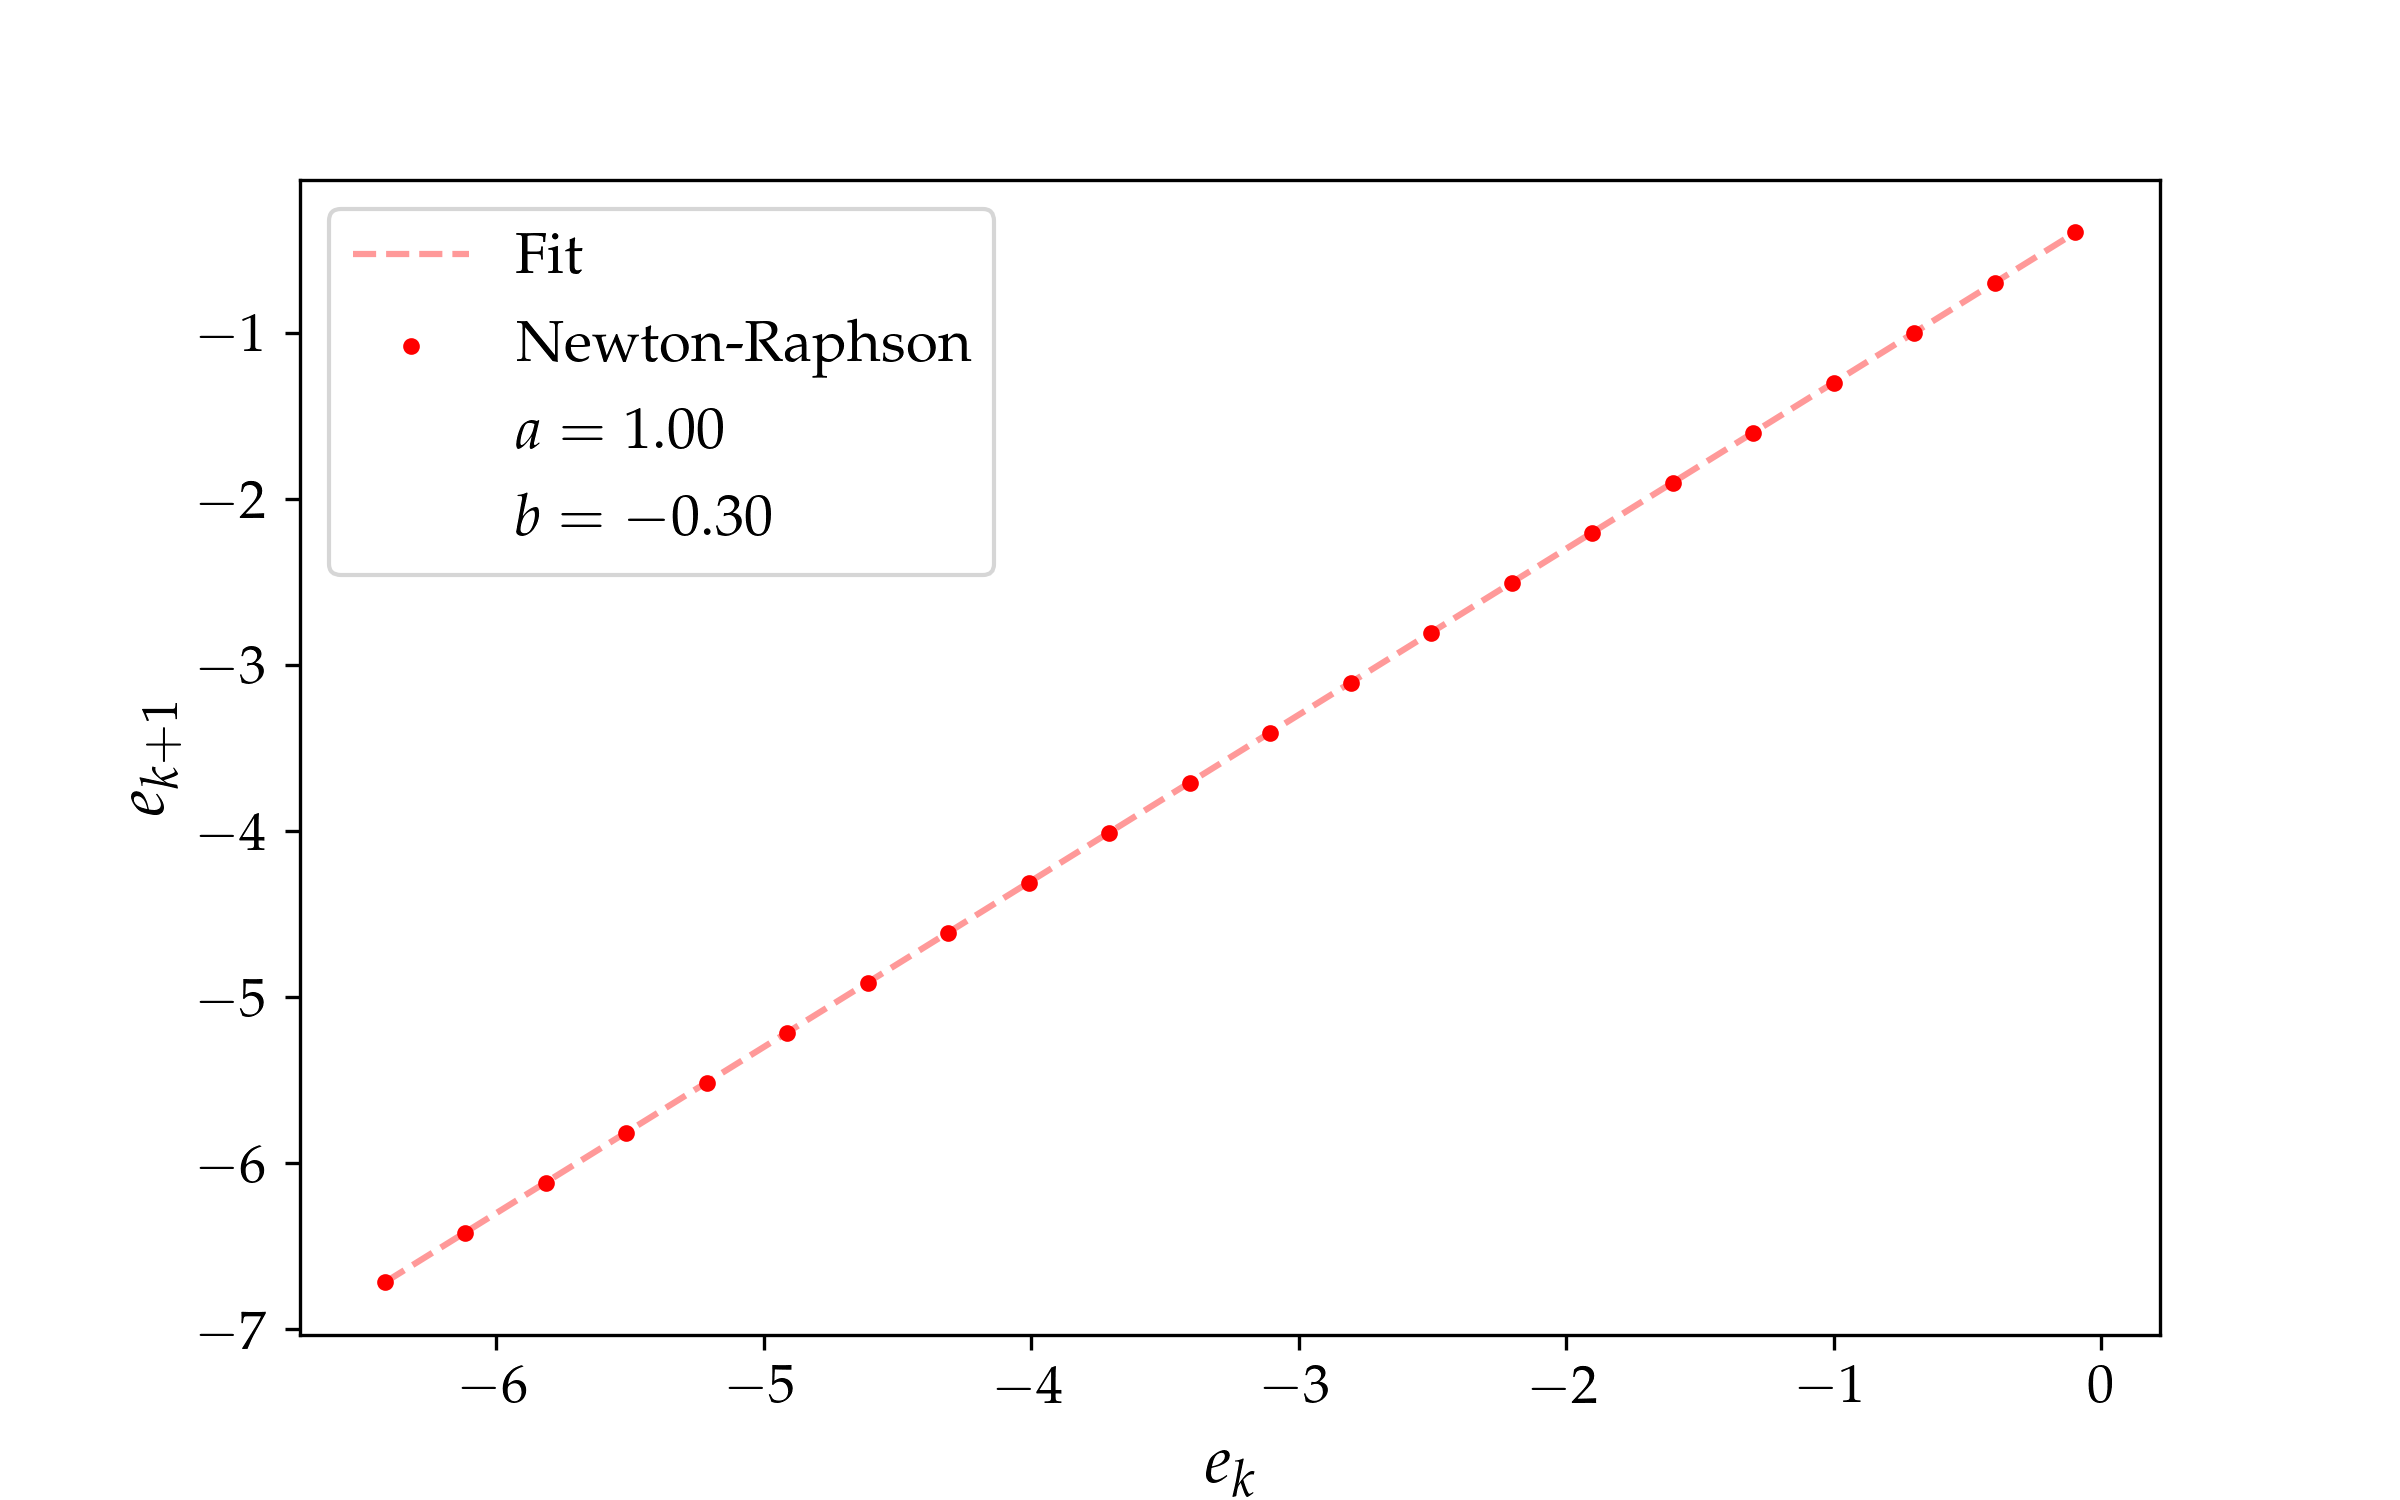
\includegraphics[width=0.8\linewidth]{images/13/fit_NR_lin.png}
    
    \caption{Convergenza in funzione del numero di iterazioni dell'algoritmo di Newton-Raphson. Per l'intestazione degli assi vale la stessa approssimazione di Fig. \ref{fig: fit Bis}.}
    \label{fig: fit NR lin}
\end{figure}


\subsubsection{Cicli}
Il secondo caso che analizziamo è quello della funzione 
\[
f(x) = x^3 -2x + 2
\]
La richiesta è di studiare l'andamento con condizioni iniziali $x_0 = 0$ e $x_0 = 1$, verificando che il metodo oscilla indefinitivamente tra i due valori, senza mai convergere alla soluzione.\\ 
L'analisi che propongo studia il comportamento in funzione di $x_0 \in [0, 1]$, estremi inclusi, osservando come per punti intermedi il metodo converga, e per i due limiti si osservi il fenomeno descritto nella consegna:\\
la soluzione analitica è:

\[
x = \sqrt[3]{-1 + \frac{\sqrt{57}}{9}} + \sqrt[3]{-1 - \frac{\sqrt{57}}{9}} \approx -1.7693
\]

\noindent In Fig. \ref{fig: NR conv 0,1} una chiara rappresentazione del fenomeno.

\medskip\noindent
Una semplice spiegazione può essere data osservando la definizione analitica dell'algoritmo e studiando cosa accade per $x_0=0,1$.\\
\begin{align*}
    f(x) &= x^3 - 2x +2\ \quad\quad
    \begin{cases}
    f(0) = 2 \\
    f(1) = 1
    \end{cases}\\
    f'(x) &= 3x^2 - 2 \quad\quad\quad\quad 
    \begin{cases}
    f'(0) = -2 \\
    f'(1) = 1
    \end{cases}\\
\end{align*}
\[
\frac{f(0,1)}{f'(0,1)} = \begin{cases}
    x_0 = 0 \implies -1 \\
    x_0 = 1 \implies +1 \\
\end{cases}
\]
\begin{align*}
    \begin{cases}
        x_1 = 0 + 1 = 1, \quad x_0=0\\
        x_1 = 1 - 1 = 0, \quad x_0=1
    \end{cases}
    \quad \implies \quad
    \begin{cases}
        x_n=0 \implies x_{n+1} =1 \\
        x_n=1 \implies x_{n+1} =0
    \end{cases}
\end{align*}

\noindent Da qui l'oscillazione tra i due valori.\\
In pratica il problema si evita modificando la stima iniziale oppure adottando versioni smorzate del metodo di Newton, per esempio:
\[
x_{n+1} = x_n - \lambda\frac{f(x_n)}{f'(x_n)}\ , \quad 0<\lambda<1
\]
che riducono il rischio di cicli e divergenze. Stiamo sostanzialmente ridefinendo il metodo per proiettare il prossimo punto dell'iterazione, non nello zero della retta tangente $x_n$, ma spostando questo punto in maniera leggera più avanti o indietro: in questo modo evitiamo una ciclicità sistematica connaturata riscontrabile con la versione non controllata dell'algoritmo.
È stata studiata questa proposta in Fig. \ref{fig: NR conv correction}, impostando $\lambda=0.85$: i risultati mostrano chiaramente come si riesca a raggiungere la convergenza con tutti gli \textit{starting point}, compresi quelli problematici di $x_0=0, 1$.

\bigskip
\begin{figure}[H]
    \centering
    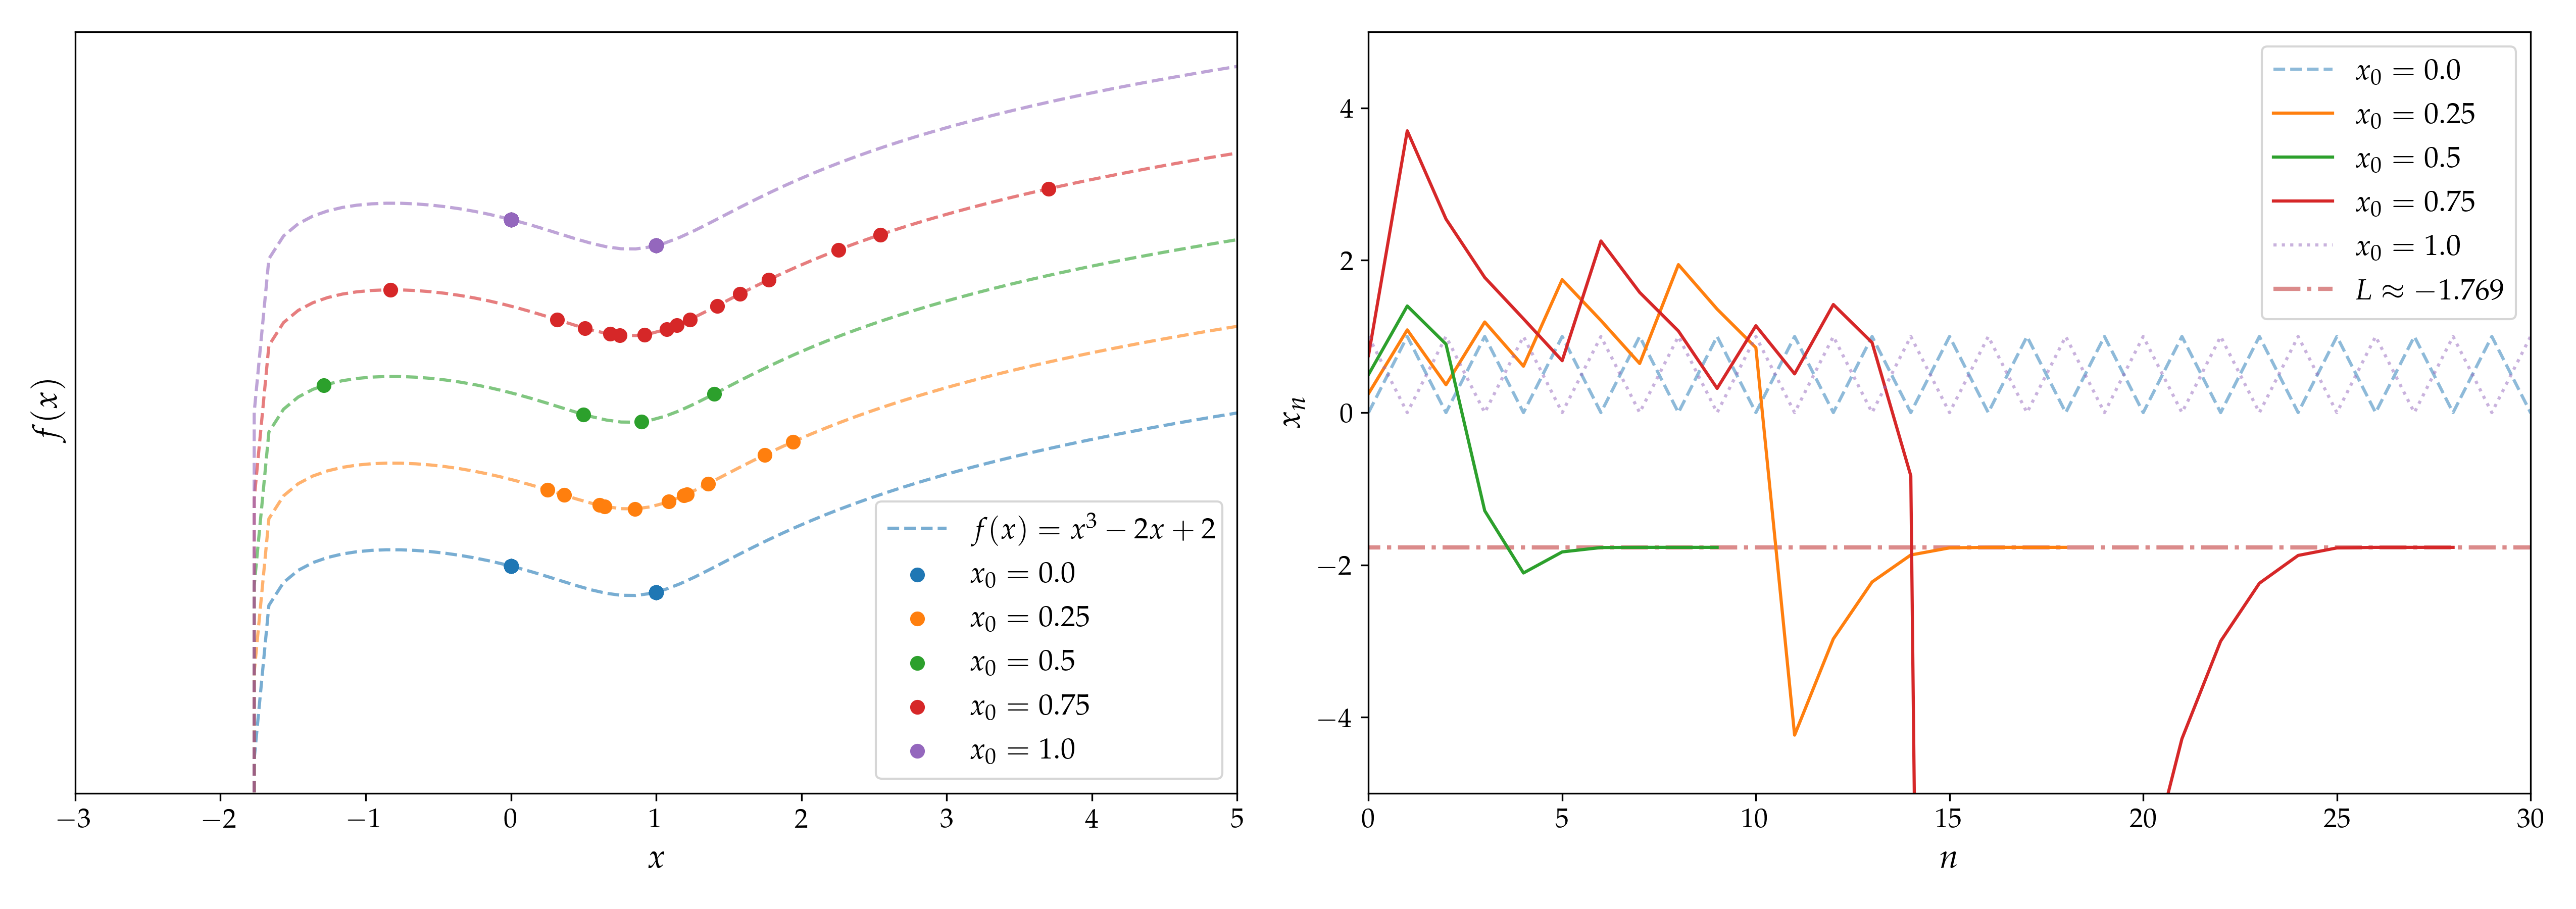
\includegraphics[width=0.9\linewidth]{images/13/fn_plot.png}
    \caption{La figura mostra a sinistra il plot di $f(x)$, con l'asse y con scala $\log_{10}$: è stato possibile moltiplicare per un fattore $n\cdot 10$ per spostare di $n$ unità in alto le linee e i punti, evitando la sovrapposizione. Ai diversi colori corrispondono diverse condizioni iniziali, con un range di $x_0 \in [0, 1]$.\\
    Nel grafico a destra si rappresenta la storia dell'algoritmo, per mostrare come procede la convergenza in funzione del numero di iterazioni: per tutti i punti intermedi è possibile terminare il programma con una stima di $L$, mentre nel caso di $x_0=0, 1$ si nota l'oscillazione indefinita tra i due valori.}
    \label{fig: NR conv 0,1}
\end{figure}

\begin{figure}[H]
    \centering
    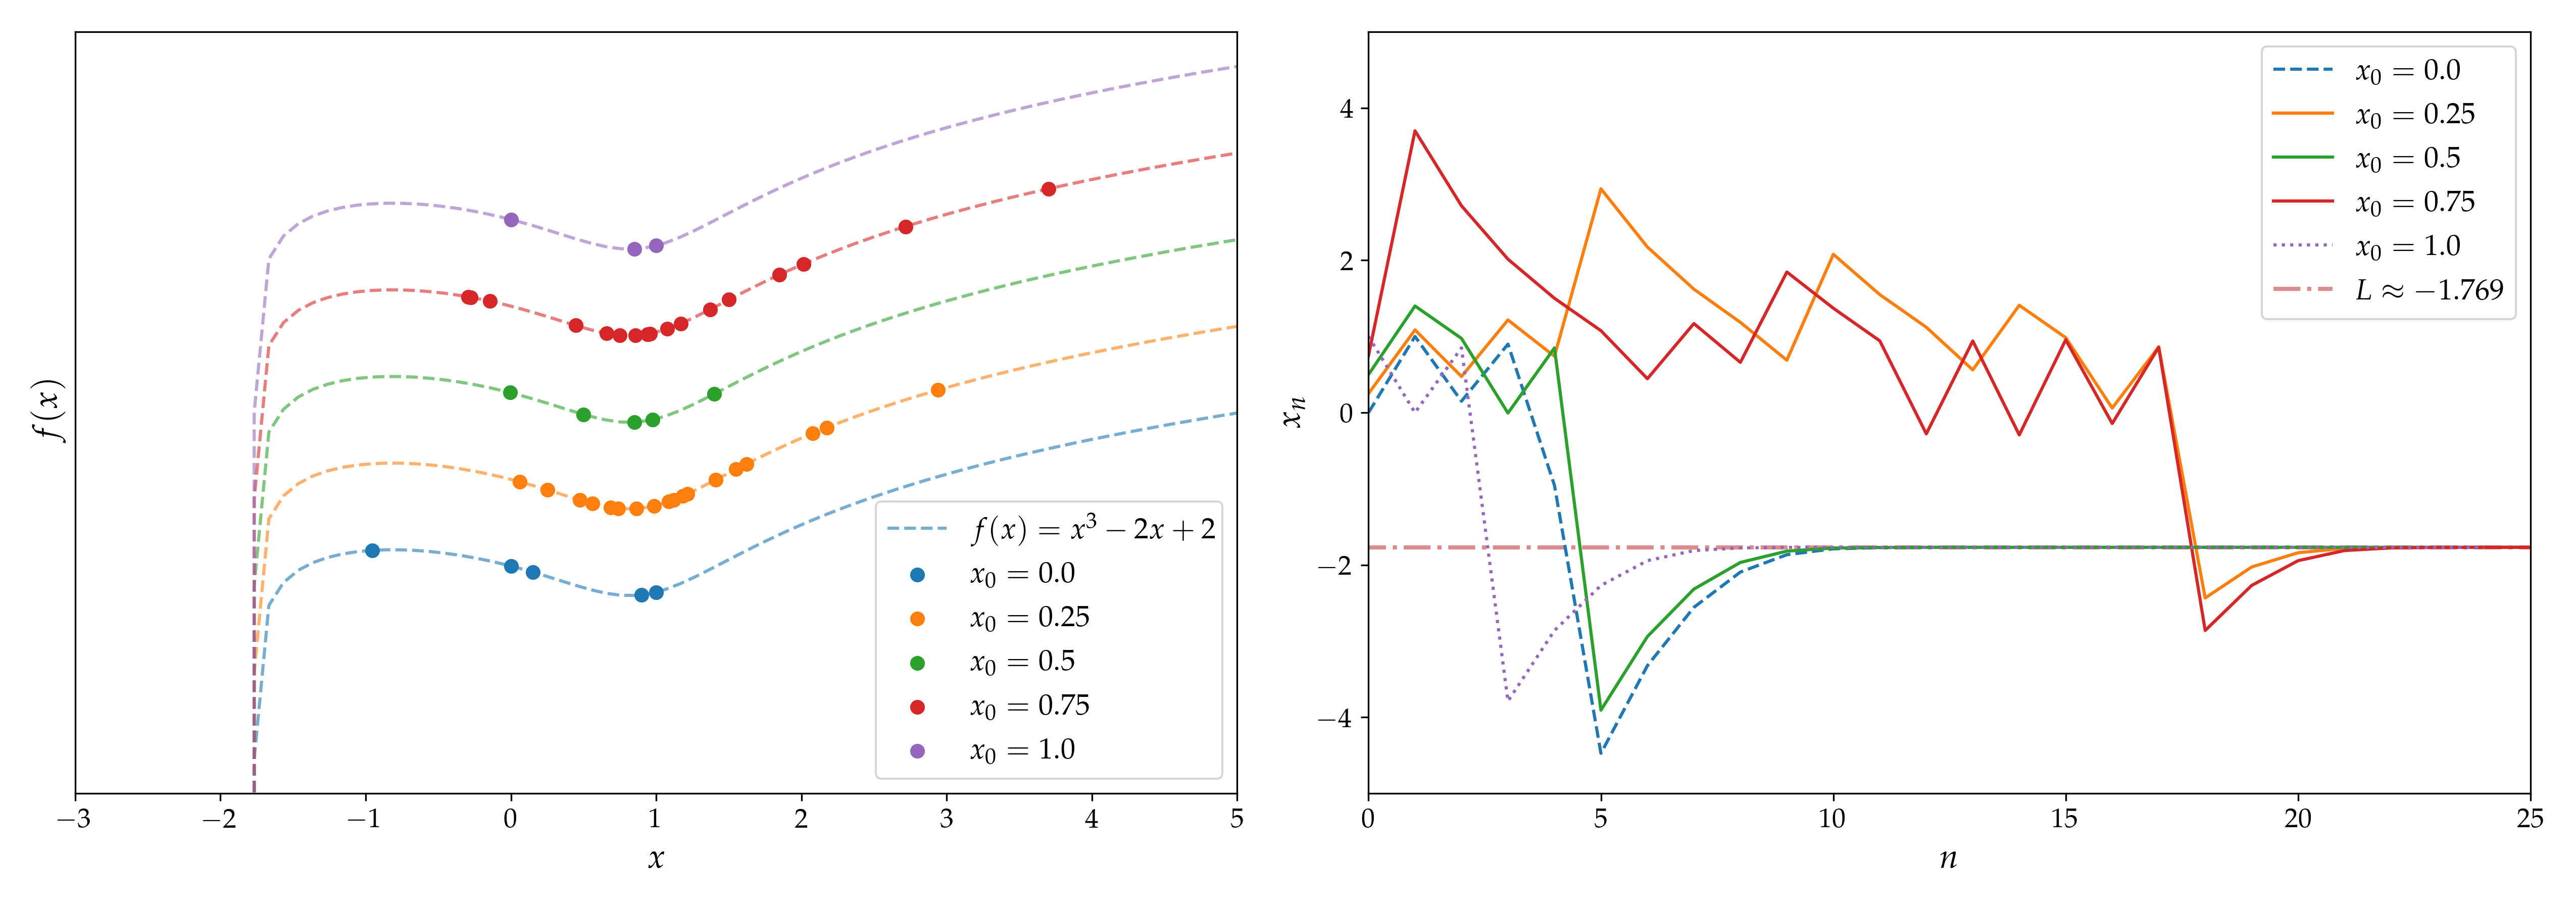
\includegraphics[width=0.9\linewidth]{images/13/fn_plot_correction.png}
    \caption{Figura analoga a Fig. \ref{fig: NR conv 0,1}, ma valutata usando l'algoritmo di Newton con la correzione introducendo il fattore $\lambda$. È possibile osservare come venga rotta la ciclicità che portava allo stagnamento e alla non convergenza che si osservavano nell'esempio precedente.}
    \label{fig: NR conv correction}
\end{figure}


\subsubsection{Condizioni iniziali}
L'ultimo esercizio propone di approfondire il problema delle condizioni iniziali, decidendo di scegliere diversi punti con cui inizializzare la ricerca dello zero e osservare come essa converga differentemente in funzione di questi.\\
In particolare si scelga la funzione
\[
f(x) = z^4 - 1, \quad z \in \mathbb{C}
\]
che ha come zeri $c = 1, -1, i -i$: restringendo il dominio di studio al quadrato sul piano complesso $Q=[-1, 1]\times[-1, 1]$, di seguito si mostrano i risultati dell'analisi. 

\medskip
\noindent In Fig. \ref{fig: fractal err mat} vediamo il controllo che è stato fatto sui risultati dell'algoritmo: si impone di ottenere un errore massimo tra la radice valutata numericamente e la più vicina delle 4 aspettate analiticamente, che sia minore di una certa soglia, impostata a $1e-9$. Formalmente:

\[
\forall z \in Q:\quad \sigma(z) = \min(|c_z - c|), \quad c \in \{1, -1, i, -i\}
\]

\noindent Imponendo che
\[
\max(\sigma) \le \varepsilon = 1e-9
\]

\bigskip\noindent
Ogni radice possiede un proprio bacino di attrazione, ossia l'insieme dei punti iniziali che convergono a quella soluzione sotto iterazione di Newton.\\
In Fig. \ref{fig: fractal} una chiara rappresentazione della figura che
rappresenta i bacini di attrazione delle quattro radici. 
La complessa geometria dei confini tra tali regioni è responsabile dell'elevata sensibilità alle condizioni iniziali: essa possiede una struttura frattale: ingrandendo queste regioni continuano a comparire dettagli complessi a scale sempre più piccole.\\

\noindent $\forall z\in Q$ viene inizializzato il metodo di N-R e della soluzione $c_z$ viene disegnato l'argomento $\theta = \arg(c_z)$ con una mappa di colore. 
Il valore di questa coordinata polare si trova nell'intervallo $[-\pi, \pi]$, ed è mostrato sulla scala di colori: il problema che si riscontra è che la scelta della libreria \textit{numpy} è di gestire gli angoli delle variabili \textit{complex} usando il branch cut lungo l'asse $\Re(z)<0$, cioè appunto l'intervallo di angoli $[-\pi, \pi]$: in questa maniera, le piccole deviazioni della posizione della radice sul piano si trasformano in notevoli differenze nel valore dell'argomento, in base che essa si trovi leggermente sopra o sotto l'asse reale (la rappresentazione del fenomeno è espressa in Fig. \ref{fig: wrong_fractal}).

\medskip
\noindent La scelta che ho fatto per risolvere questo problema è stata quella di usare una colormap ciclica, cioè che riportasse gli stessi colori sugli estremi della scala: in questo modo a $\arg(z)=\pm \pi$ viene associata effettivamente la stessa colorazione.

\begin{figure}[H]
    \centering
    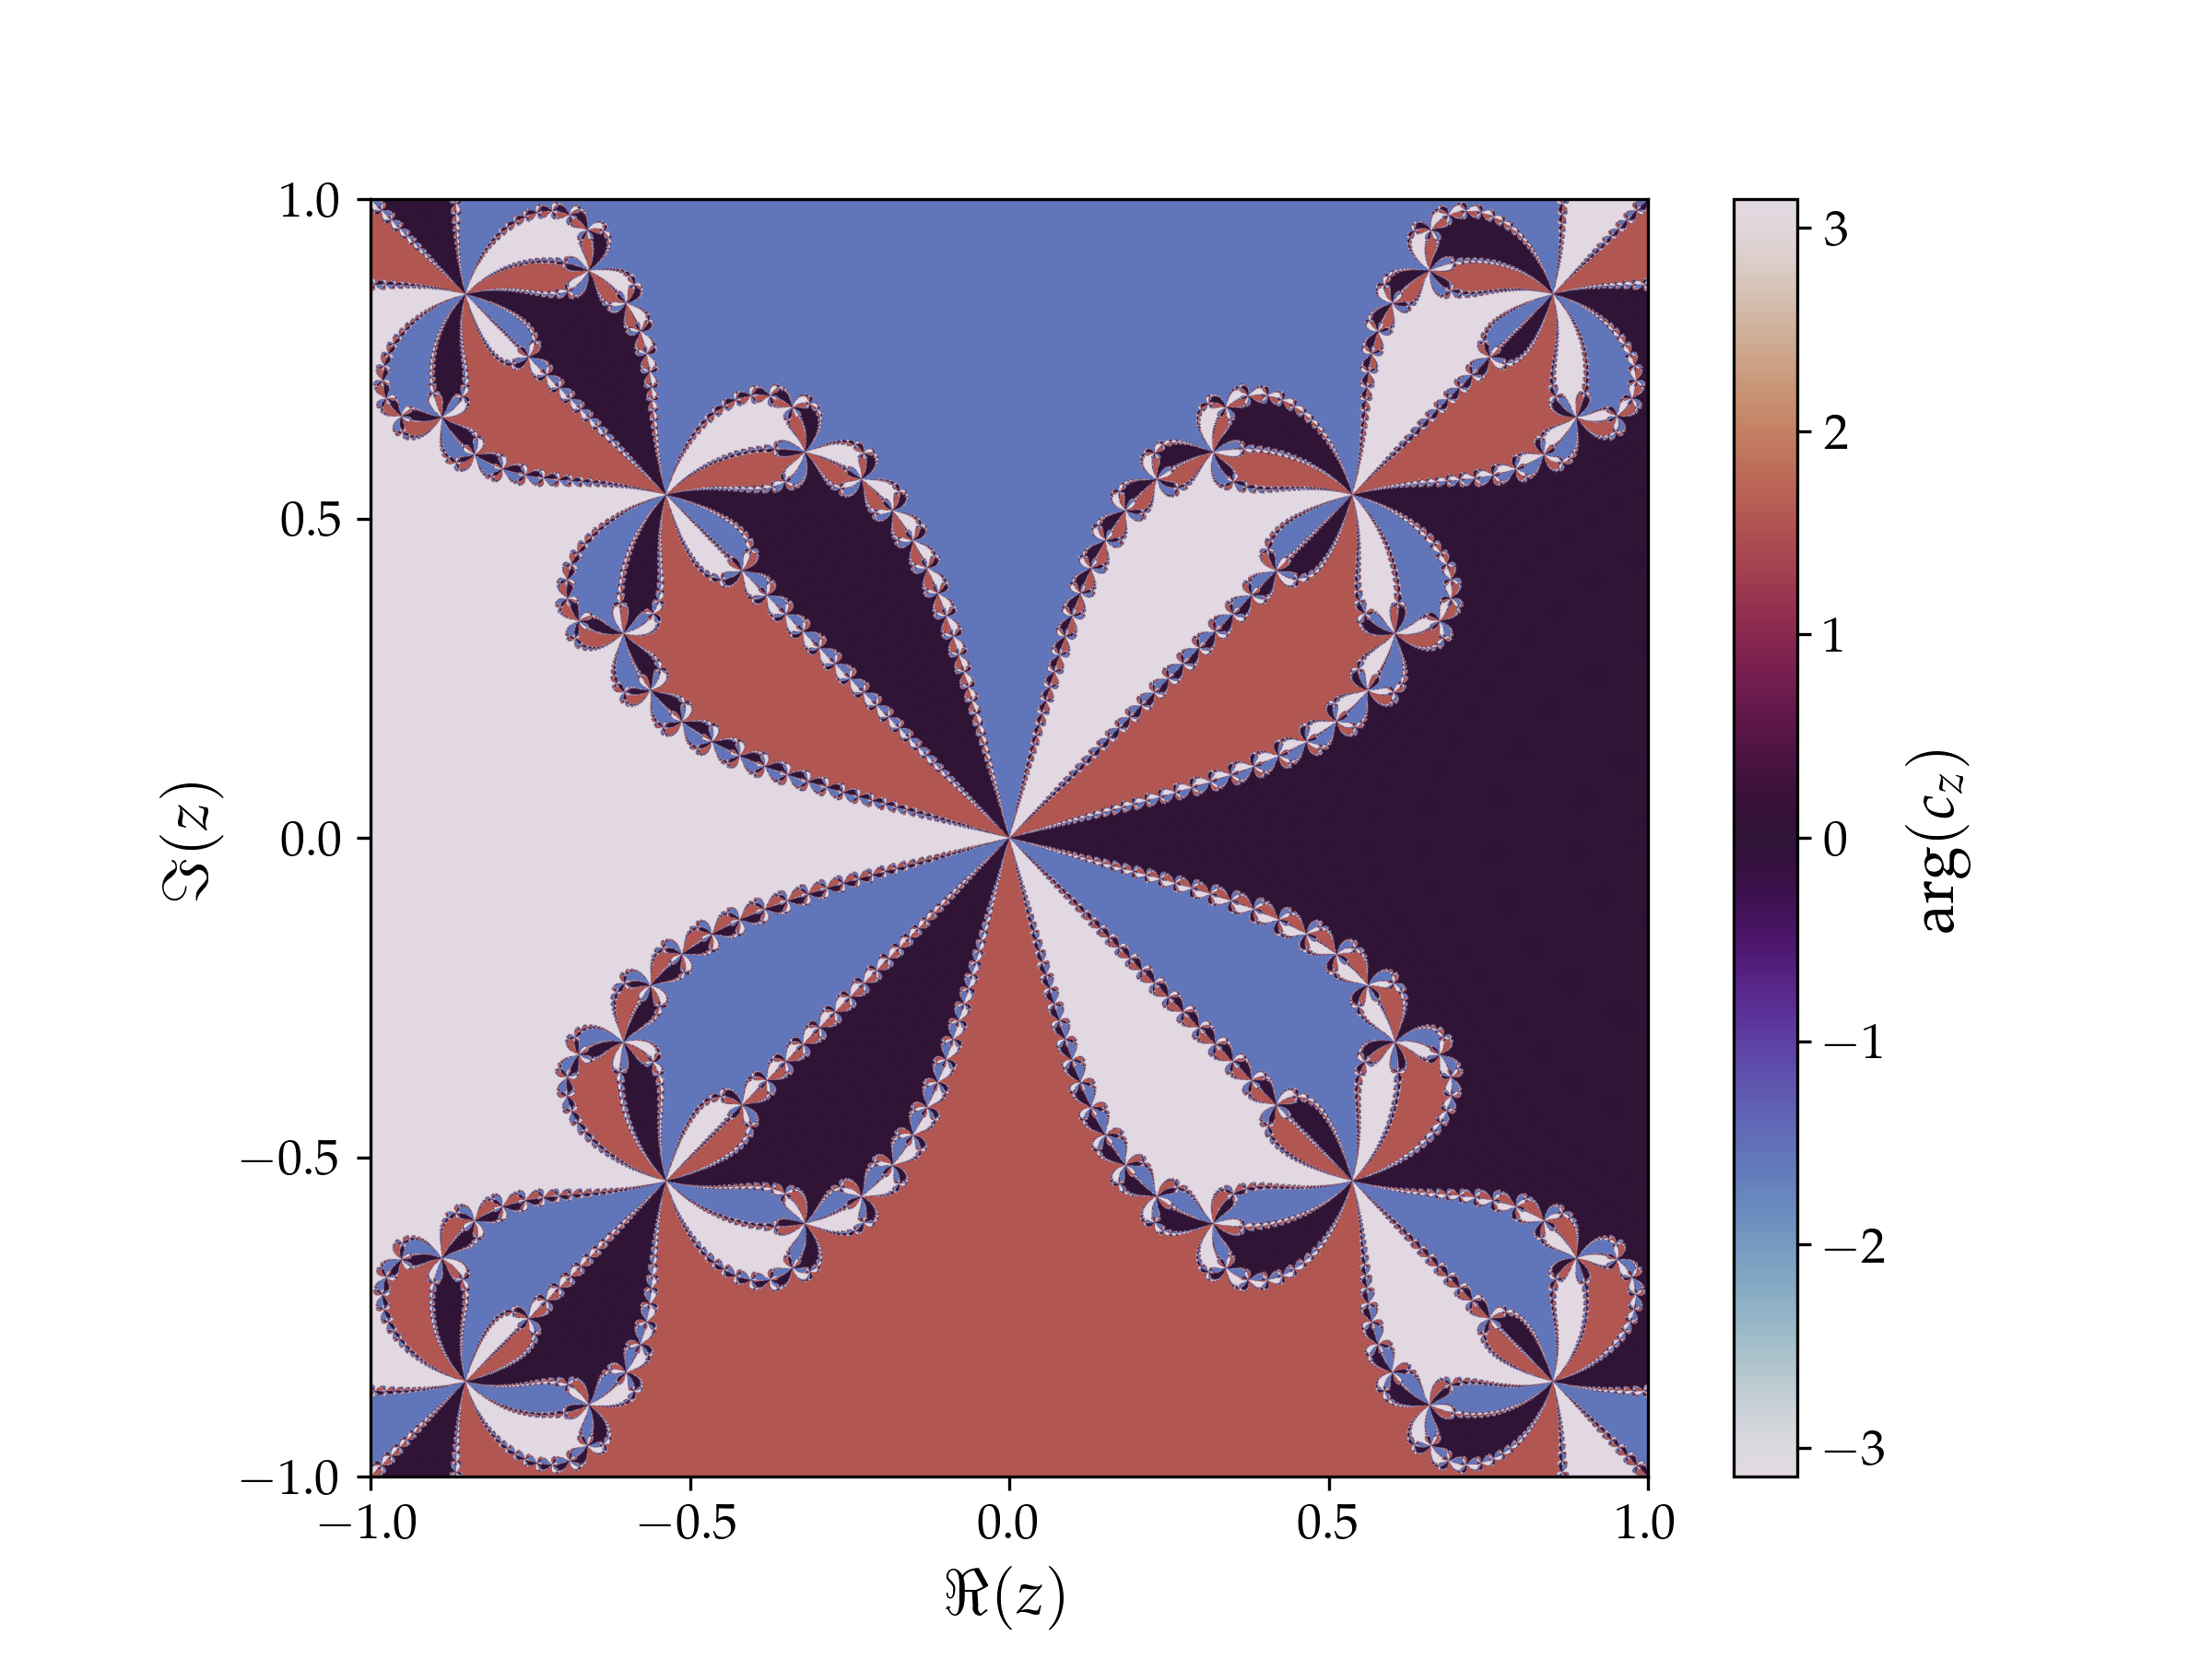
\includegraphics[width=0.75\linewidth]{images/13/fractal.png}
    \caption{La figura frattale che risulta dal plot dell'argomento della radice complessa che si ottiene impostando come $z_0$ un determinato punto $z$ del piano di Argand-Gauss. La scala di colori continua si riduce ad essere sostanzialmente discreta, poiché vengono selezionati solamente i quattro colori relativi alle soluzioni ($\theta = 0, \pm \pi, \pm\pi/2$).}
    \label{fig: fractal}
\end{figure}
\begin{figure}[H]
    \centering
    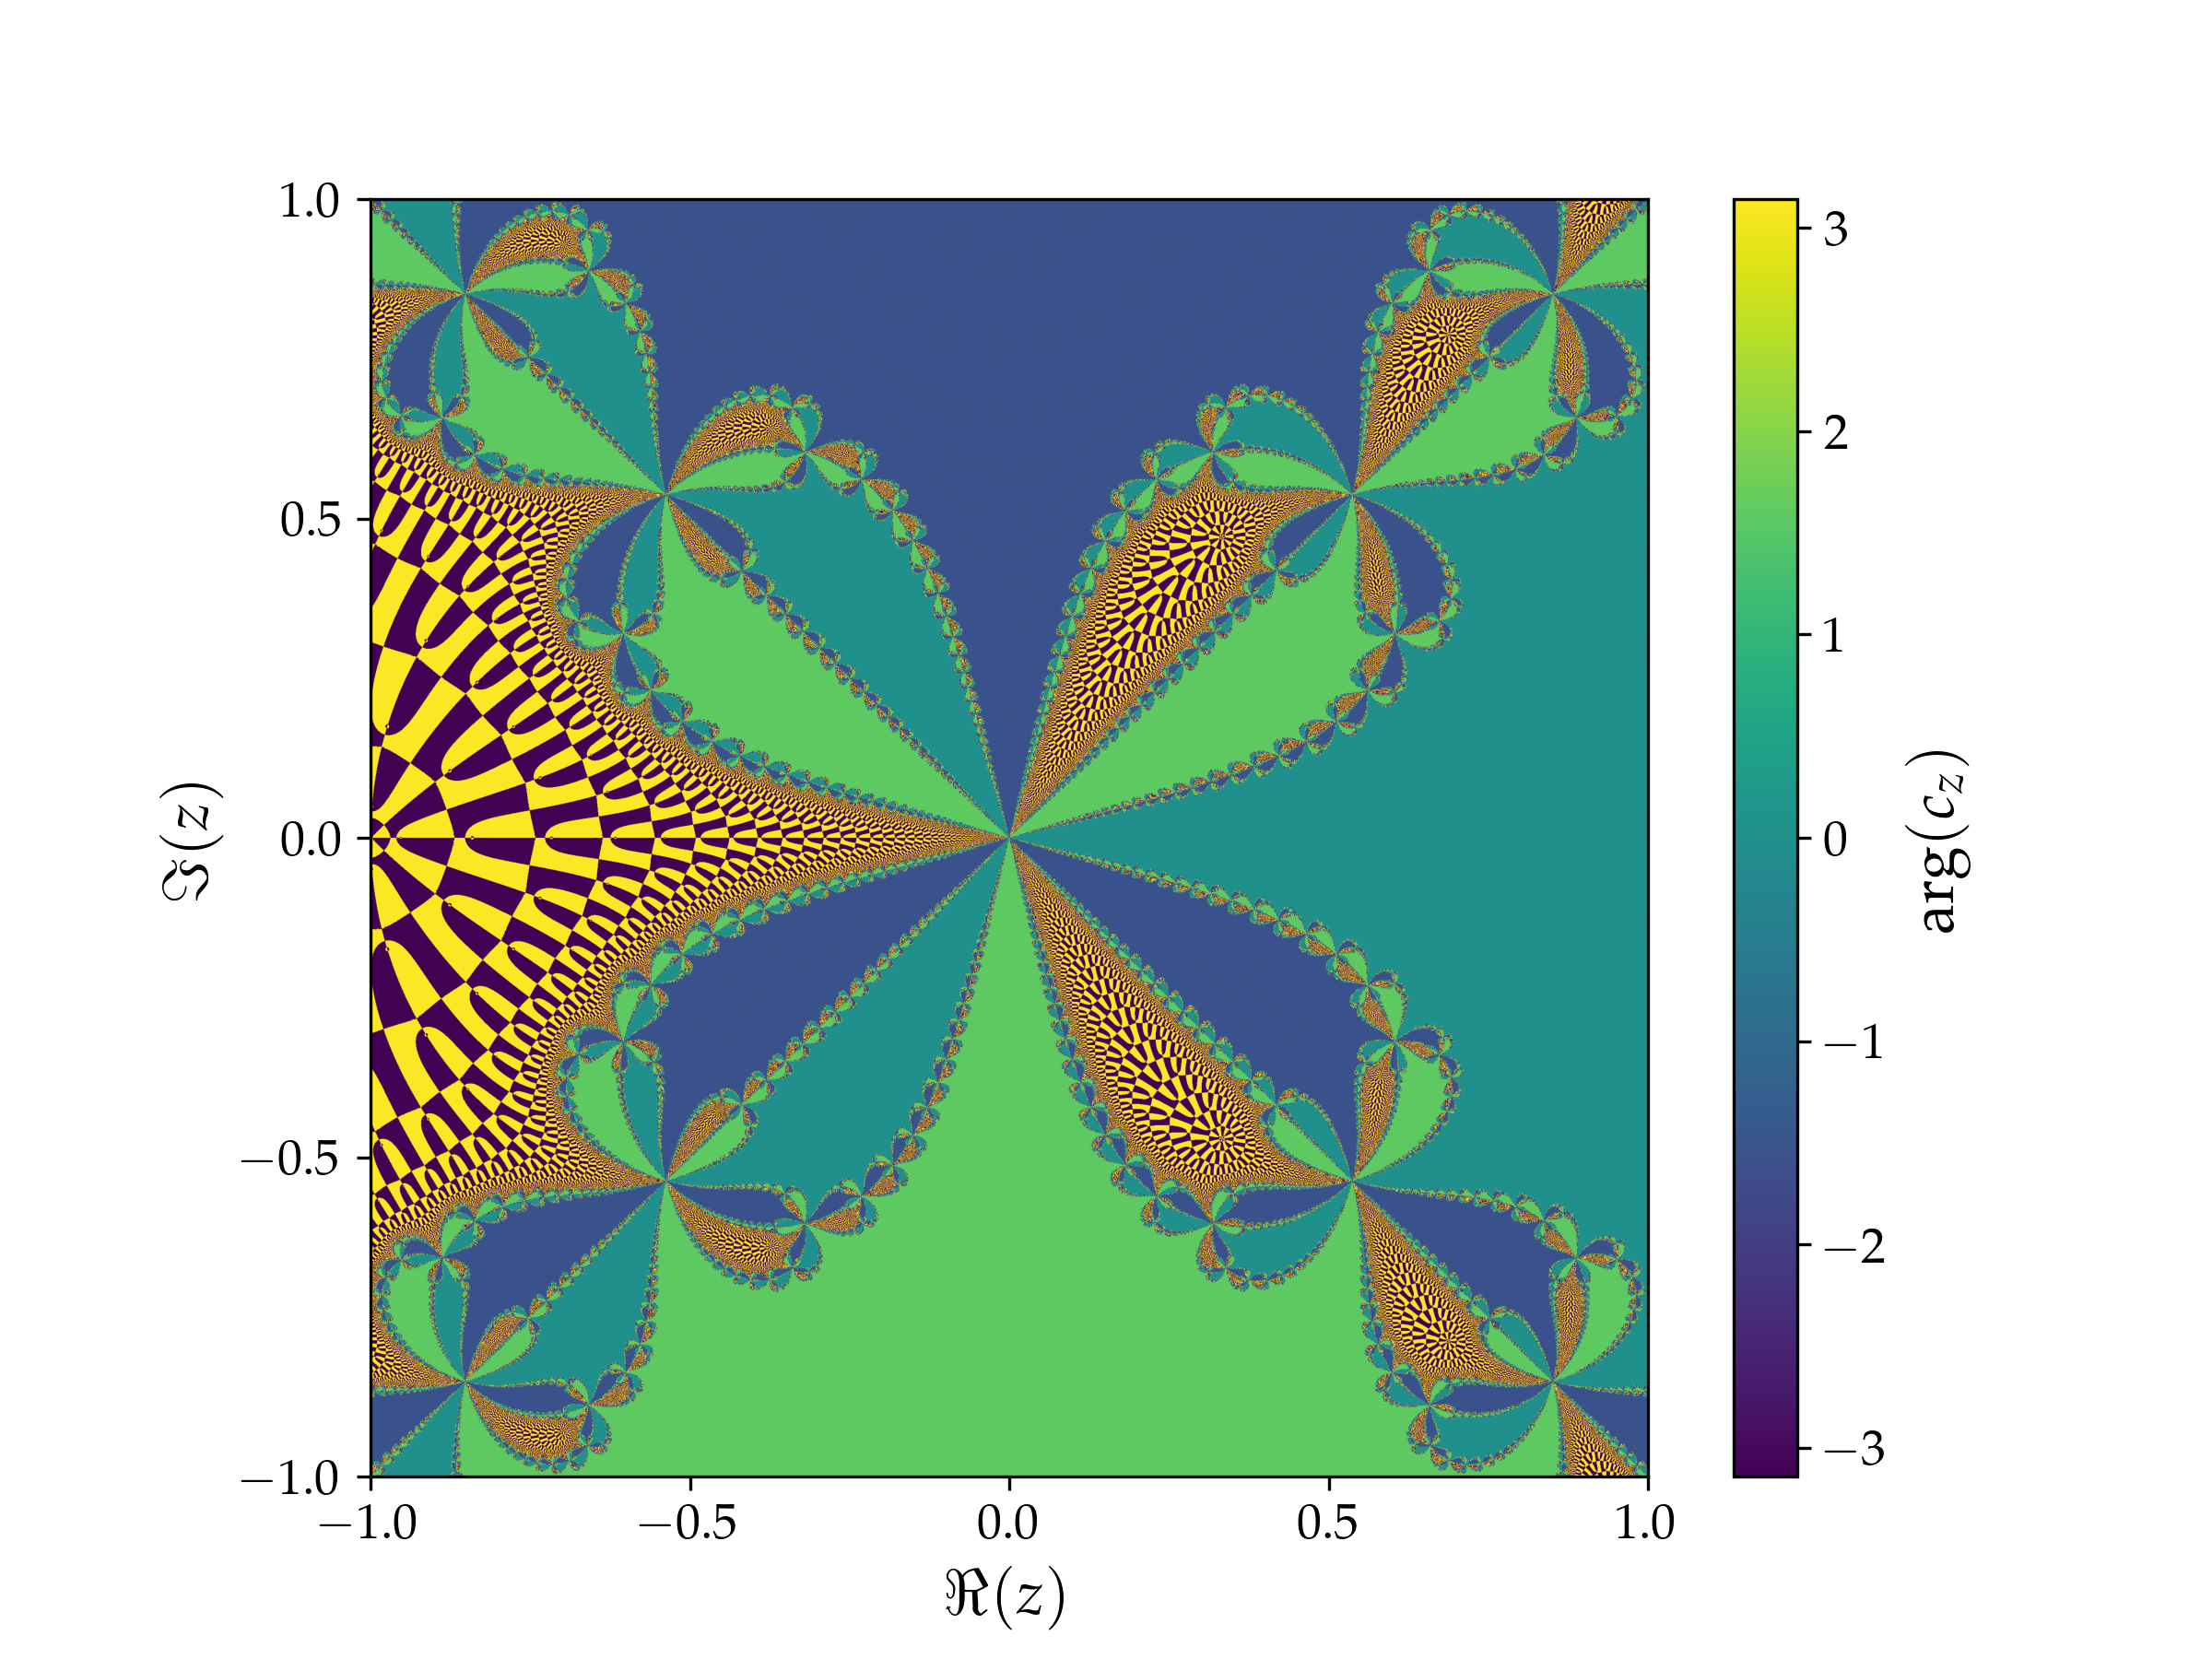
\includegraphics[width=0.75\linewidth]{images/13/wrong_fractal.png}
    \caption{La figura rappresenta, usando una colormap sequenziale come \textit{viridis}, che gli errori sulla ricerca della radice $-1$ comportano un certo grado di ambiguità sul valore dell'argomento di $c_z$.}
    \label{fig: wrong_fractal}
\end{figure}


\begin{figure}[H]
    \centering
    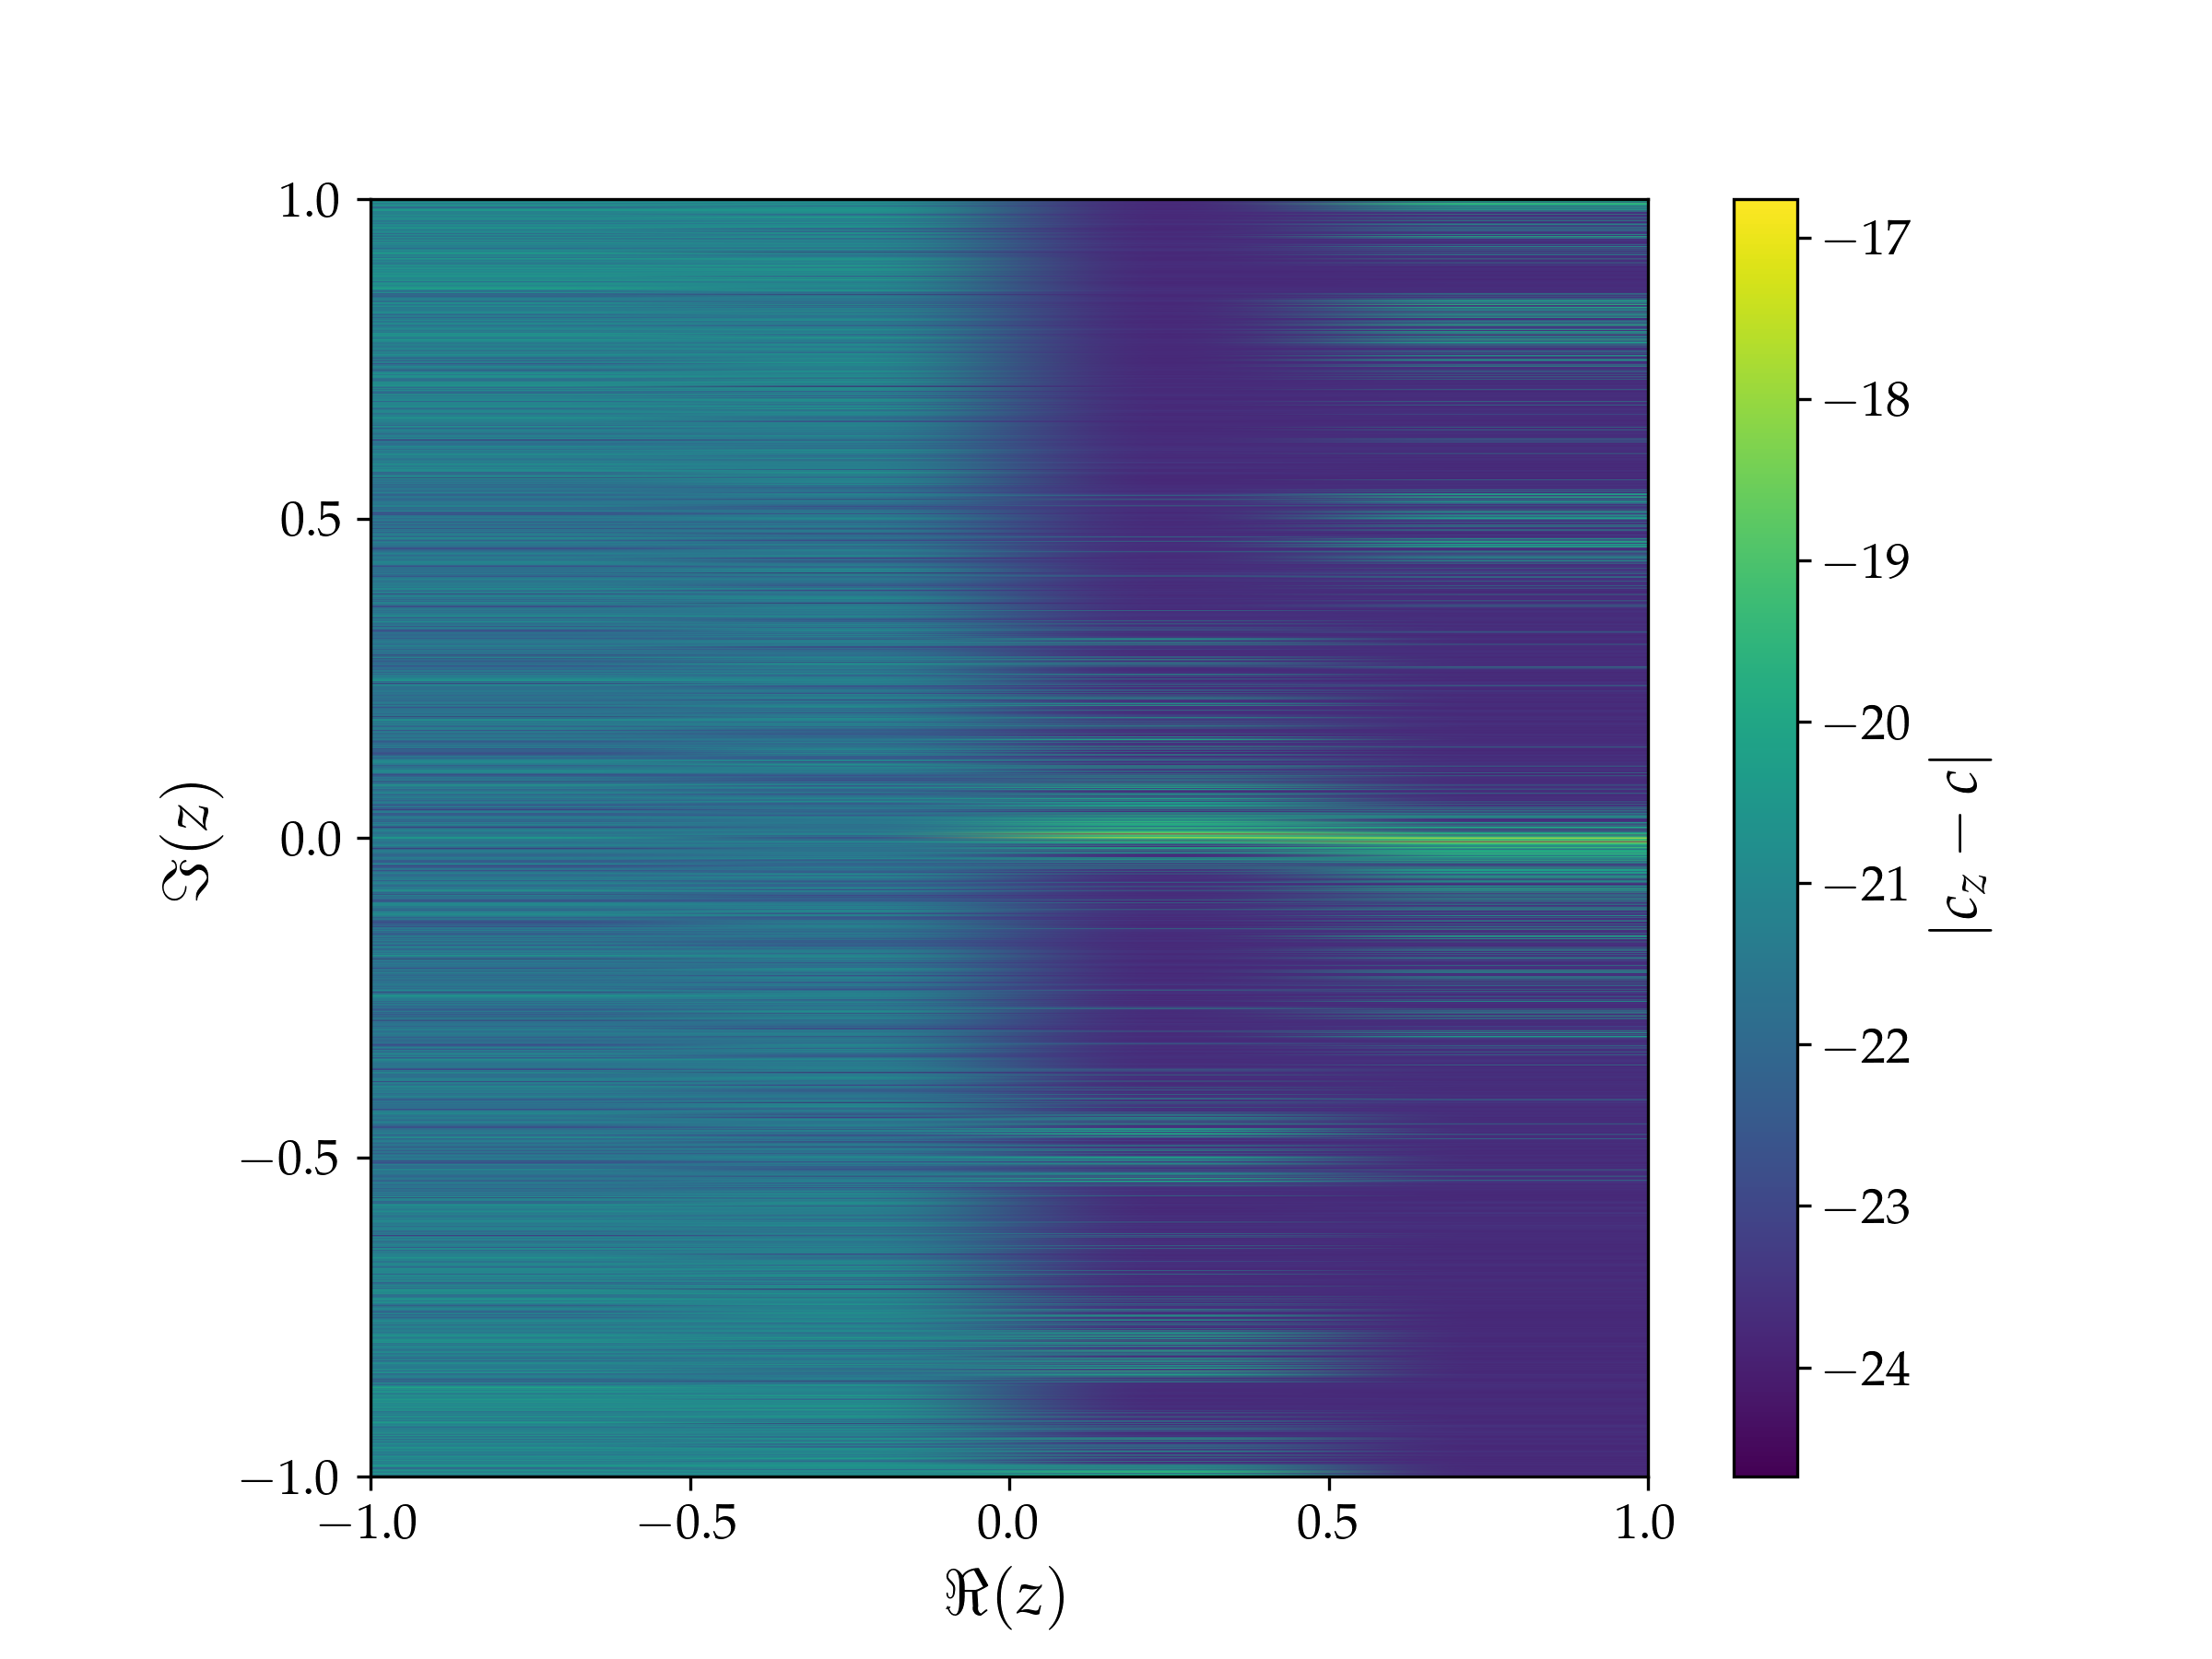
\includegraphics[width=0.8\linewidth]{images/13/error_matrix.png}
    \caption{Mappa della distanza (errore) rispetto alla radice più vicina: la scala logaritmica mostra che gli errori sono globalmente piccoli (è stato impostato un fondo scala di $1e-25$ per evitare possibili coincidenze $c_z=c$). Questo errore è ottenibile grazie ad una correzione che viene applicata sul metodo di Newton: per evitare la singolarità in $z=0$ ho introdotto una regolarizzazione numerica $f'(z+\epsilon)$, dove $\epsilon=1e-5$ è la più piccola deviazione che permette di avere un errore massimo sotto la tolleranza di $\text{Max err} \le 1e-9$. In questo esempio otteniamo $\text{Max err} = 1.73e-17<1e-9$.\\
    Questa modifica non fa parte del metodo di Newton standard ma è stata utilizzata esclusivamente per stabilizzare il calcolo sulla griglia discreta.}
    \label{fig: fractal err mat}
\end{figure}


\newpage












\section{Esercizio 5.2.3}
\subsection{Problem Statement}
Risolvi le equazioni trascendenti per $\hbar = 1, m = L = 1$ e $V_0 = 10$ utilizzando gli algoritmi di bisezione, Regula Falsi e Newton-Raphson/Secante. Sentiti libero di decidere se vuoi calcolare a mano le derivate prime o se invece vuoi utilizzare il metodo della Secante.

\vspace{1em}
\begin{enumerate}
    \item Trova la radice di $f_{\text{pari}}$ e confronta il tasso di convergenza dei tre metodi (studiando $|c - c_{\text{esatto}}|$ e $|f(c)|$ in funzione delle iterazioni in un unico grafico). Usa un intervallo ragionevole nella regione al di sotto di $-6$ per i metodi di bracketing e $x_0 < -6$ per quello di Newton.
    
    \item Dimostra che la convergenza è lineare per il metodo di bisezione e quadratica per il metodo di Newton partendo dai dati raccolti.
    
    \item Prova a scegliere diversi valori iniziali a destra della discontinuità per il metodo di Newton, nello specifico nell'intervallo $[-5.2, -5.0]$ e monitora, ovvero traccia un grafico, della soluzione per le prime 10-20 iterazioni. Cosa impari?
    
    \item Traccia il grafico dell'equazione trascendente dispari per individuare approssimativamente le altre radici. Quindi passa un intervallo di input ragionevole ai metodi di bracketing e un'ipotesi di partenza ragionevole per l'algoritmo di Newton.
\end{enumerate}

\subsection{Premessa Teorica}
Per una massa $m$ le funzioni d'onda nella buca di potenziale finita ($-\infty <V_0<+\infty$) 1-dimensionale sono descritte da delle equazioni trascendenti, non risolvibili analiticamente, ma che richiedono una soluzione numerica. Lo spettro dei livelli energetici è discreto e definito da $E$: questa configurazione è detta di \textit{stato legato}.\\
Per gli stati pari vale la seguente equazione:
\[
k(E) \tan\left(\frac{k(E) L}{2}\right) = \bar\kappa(E)
\]

mentre per quelli dispari:
\[
k(E) \cot\left(\frac{k(E) L}{2}\right) = -\bar\kappa(E)
\]

considerando
\[
k(E) = \sqrt{\frac{2 m (V_0 + E)}{\hbar^2}}, \quad
\bar\kappa(E) = \sqrt{\frac{-2 m E}{\hbar^2}}
\]

\medskip\noindent
Per la risoluzione in funzione di $E$, cioè la ricerca del livello energetico, fissate le condizioni al contorno, è possibile ridefinire l'analisi come la ricerca di uno zero di $f(E)$ così definita:
\begin{align*}
f_\mathrm{pari}(E) &= k(E) \tan\left(\frac{k(E) L}{2}\right) - \bar\kappa(E)\\
f_\mathrm{dispari}(E) &= k(E) \cot\left(\frac{k(E) L}{2}\right) + \bar\kappa(E)
\end{align*}

\subsection{Metodi Numerici e Algoritmi}
Decidiamo di introdurre un nuovo algoritmo, per la ricerca degli zeri di una funzione, rivedendo la definizione del N-R, ma combinandolo con queste caratteristiche:
\begin{itemize}
    \item Evitare il calcolo analitico della derivata, che può, in alcuni casi, essere complesso o dispendioso.
    \item Avere un rate di convergenza maggiore rispetto a quello lineare della bisezione o Regula Falsi.
    \item Massimizzare l'efficienza computazionale, ottimizzando al massimo le valutazioni della funzione, soprattutto in caso che essa sia molto complessa e computazionalmente pesante.
\end{itemize}

Nasce così il \textit{Metodo delle Secanti}, che rispecchia proprio queste tre caratteristiche.
Partendo dal ben conosciuto algoritmo di Newton-Raphson, possiamo decidere di ridefinire la derivata prima, non come funziona analitica, ma usando le derivate finite, in particolare la definizione \textit{backward}:
\begin{align*}
\frac{f(x) - f(x-\epsilon)}{\epsilon} & = f'(x) + O(\epsilon) \\
\end{align*}
se $\epsilon$ è piccolo e rappresenta il passo dell'iterazione ($x_n - x_{n-1} = \epsilon$) il metodo N-R viene riscritto così:
\[
    x_{n+1} = x_n - f(x_n) \frac{x_n- x_{n-1}}{f(x_n) - f(x_{n-1})}
\]

Il rate di convergenza non è lineare né quadratico, ma è una via di mezzo fra questi: il metodo viene detto superlineare, poiché $1<p<2$, $p=\phi \approx1.618$. Inoltre si può osservare che mantendo in memoria $f(x_{n-1})$ dell'iterazione precedente, possiamo fare un'unica valutazione della funzione per iterazione. Questa definizione del punto $x_{n+1}$ come funzione di $x_n, x_{n-1}$ implica che l'algoritmo necessita di essere inizializzato con due punti, e non più solo uno come nel caso di N-R.

\subsection{Risultati e Discussione}
In primis si mostra un plot (Fig. \ref{fig: f even}) della funzione e della sua derivata nell'intervallo di interesse: si noti la presenza di una singolarità (asintoto verticale), che può compromettere la convergenza di Newton-Raphson e del metodo delle Secanti se l'inizializzazione cade troppo vicino alla discontinuità o conduce l'iterazione ad attraversarla.

\begin{figure}[H]
    \centering
    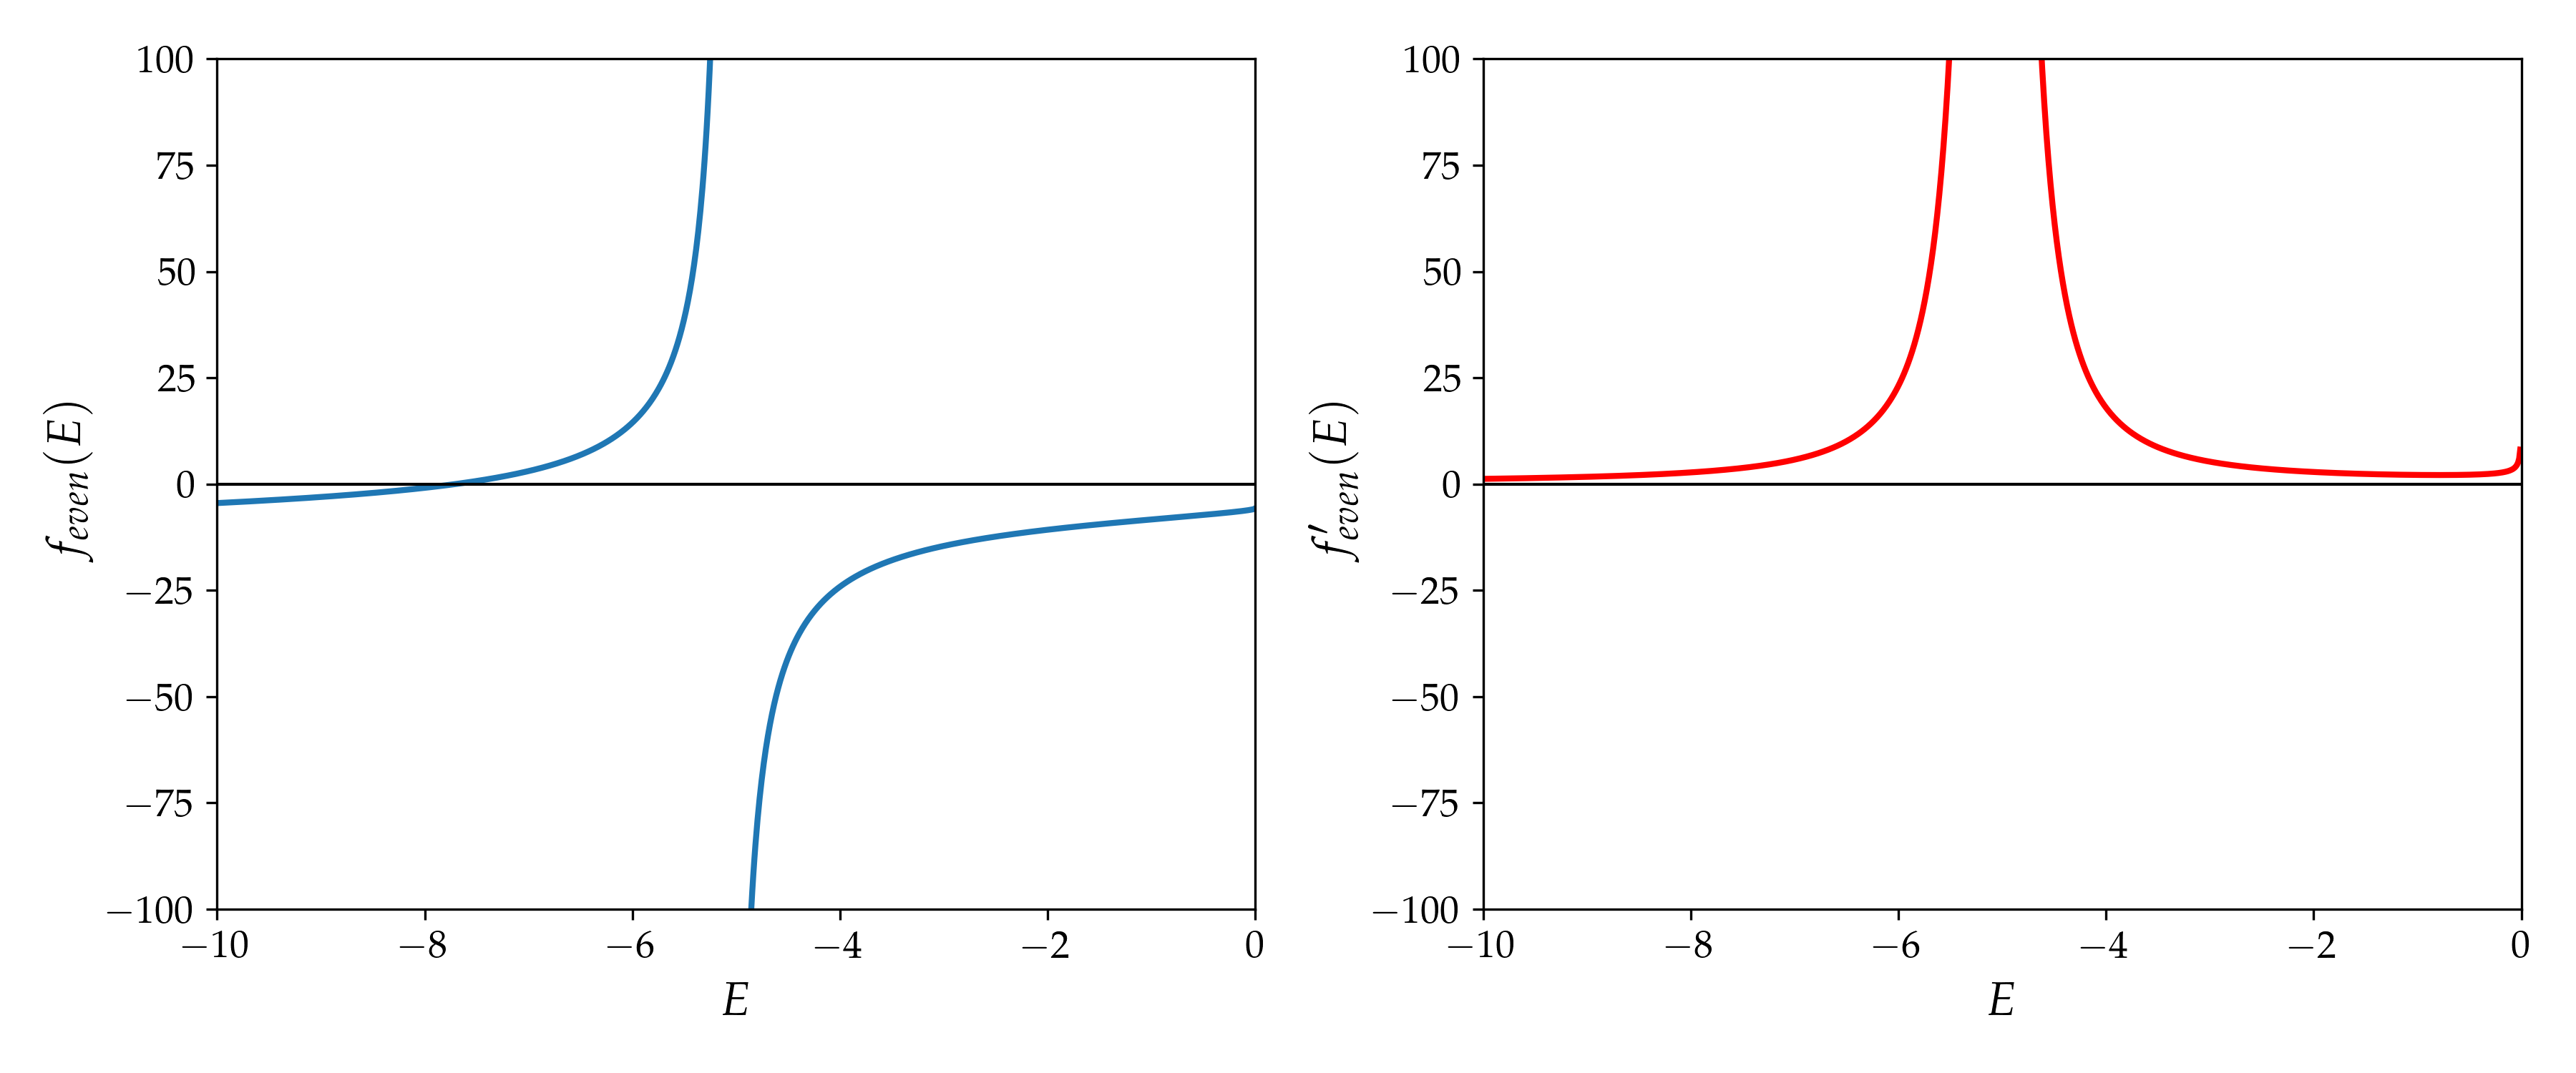
\includegraphics[width=\linewidth]{images/14/f_even.png}
    \caption{Plot della funzione pari e della sua derivata: si nota un punto di discontinuità.}
    \label{fig: f even}
\end{figure}

Vengono quindi comparati i quattro metodi presentati sino ad ora: ne studiamo la storia della radice e del valore della funzione, in termini del numero di iterazioni. Infine compariamo le convergenze e verifichiamo che si riscontrino i comportamenti aspettati.

\begin{elegantcode}[title={Risultati per i diversi algoritmi di ricerca}]
Bisection        c = -7.7050092507390815
                 iters = 47

Regula Falsi     c = -7.705009250739083
                 iters = 24

Secant           c = -7.7050092507390815
                 iters = 9

Newton-Raphson   c = -7.7050092507390815
                 iters = 8
\end{elegantcode}

È in Fig. \ref{fig: conv_even} che osserviamo una prima stima dei diversi comportamenti delle funzioni: qualitativamente è possibile vedere come Bisezione e Regula Falsi convergano in maniera lineare, mentre gli altri con una traiettoria più "parabolica", infine si nota che tra i due superlineari è Newton-Raphson ad avere la meglio e convergere più rapidamente.

\medskip\noindent
L'andamento vero e proprio delle funzioni, nella scala adatta, è fatto nei plot Fig. \ref{fig: confr even}, Fig. \ref{fig: even mean} e nei fit di Figs. \ref{fig: bisezione_fit}-\ref{fig: NR_fit} (per cui è sottinteso per ognuna l'approssimazione sull'intestazione degli assi di Fig.\ref{fig: fit Bis}.). È omessa l'incertezza legata alla stima del parametro di scaling per le considerazioni fatte, e già proposte, nell'appendice, perció non è possibile proporre i risultati del test del t-Student, poiché non attendibili come valutazioni statistiche: in particolare in Fig. \ref{fig: even mean} il valore stimato è la media aritmetica delle ascisse dei punti, statistica non rigorosa poiché i punti $e_{k+1}/e_k$ sono chiaramente non i.i.d. (indipendenti e identicamente distribuiti); per le figure riferite ai fit delle singole distribuzioni, il parametro è frutto della stima del fit con regressione lineare, ma anche in questo caso l'incertezza non è fornita, poiché viene usata la matrice di identità come covarianza (vedi Appendice).\\


\begin{figure}[H]
    \centering
    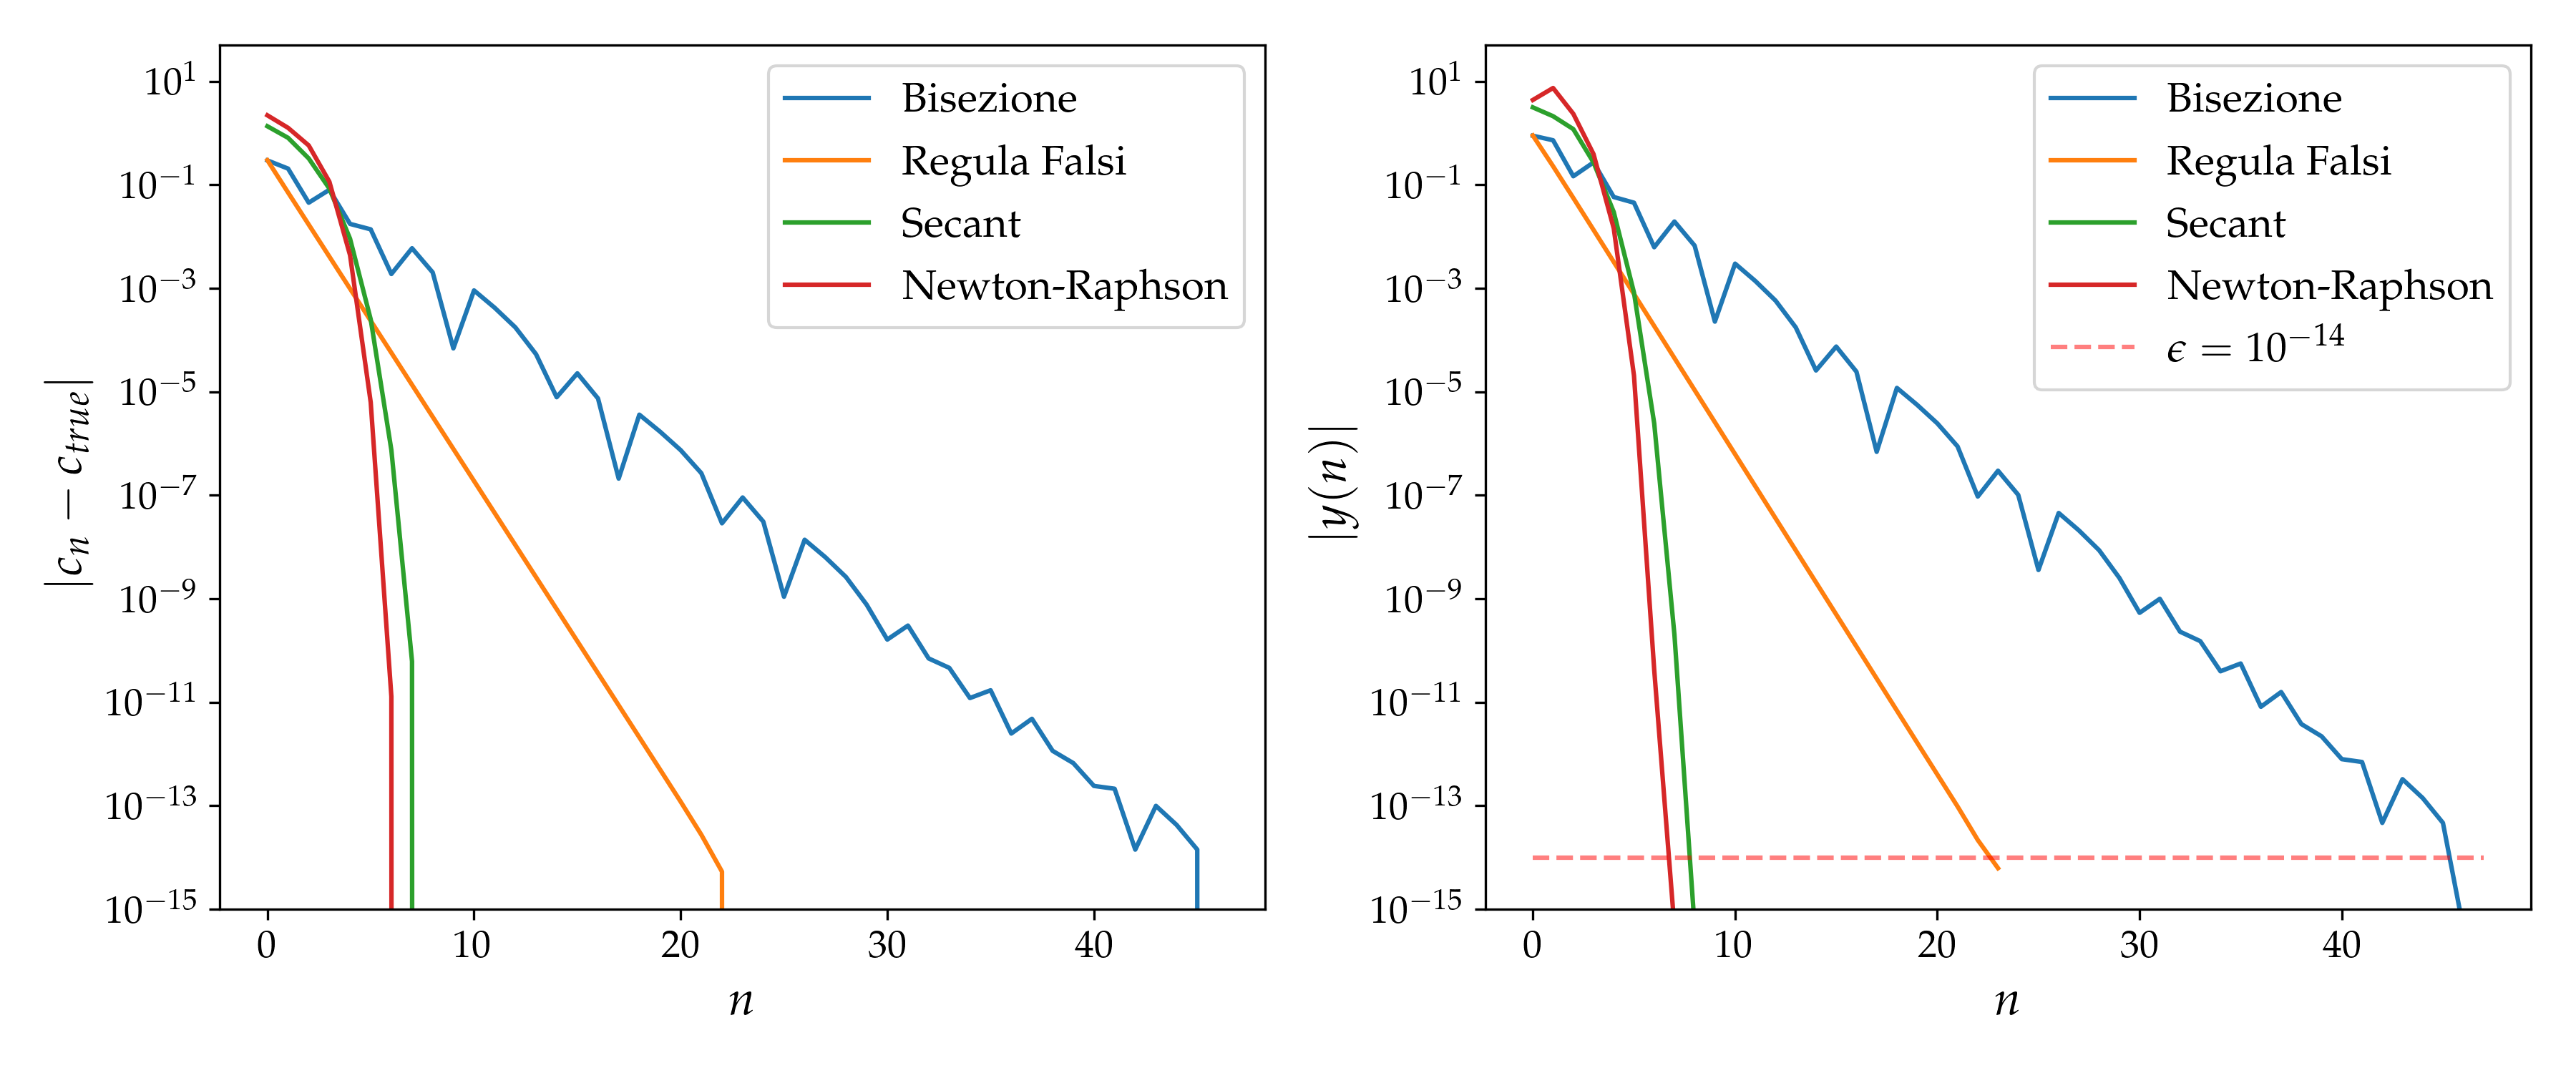
\includegraphics[width=\linewidth]{images/14/even_conv.png}
    \caption{Sulla sinistra il plot dell'errore rispetto alla radice vera (valutata come l'ultimo punto della successione, quando l'algoritmo converge e si ferma). A destra l'errore sulla funzione al passo n-esimo; sapendo che la funzione nella radice vale per definizione zero, si riduce ad essere il valore assoluto della funzione valutata nel punto $c_n$. Si noti come in questa seconda figura è anche indicata la tolleranza che è stata stabilita condivisa per tutti gli algoritmi: per definizione il metodo converge quando il valore della funzione nella \textit{guess} è minore di $\epsilon$, quindi vediamo che tutte le storie dei diversi algoritmi arrivano a convergenza e si fermano, solamente dopo aver superato questa soglia.}
    \label{fig: conv_even}
\end{figure}


\begin{figure}[H]
    \centering
    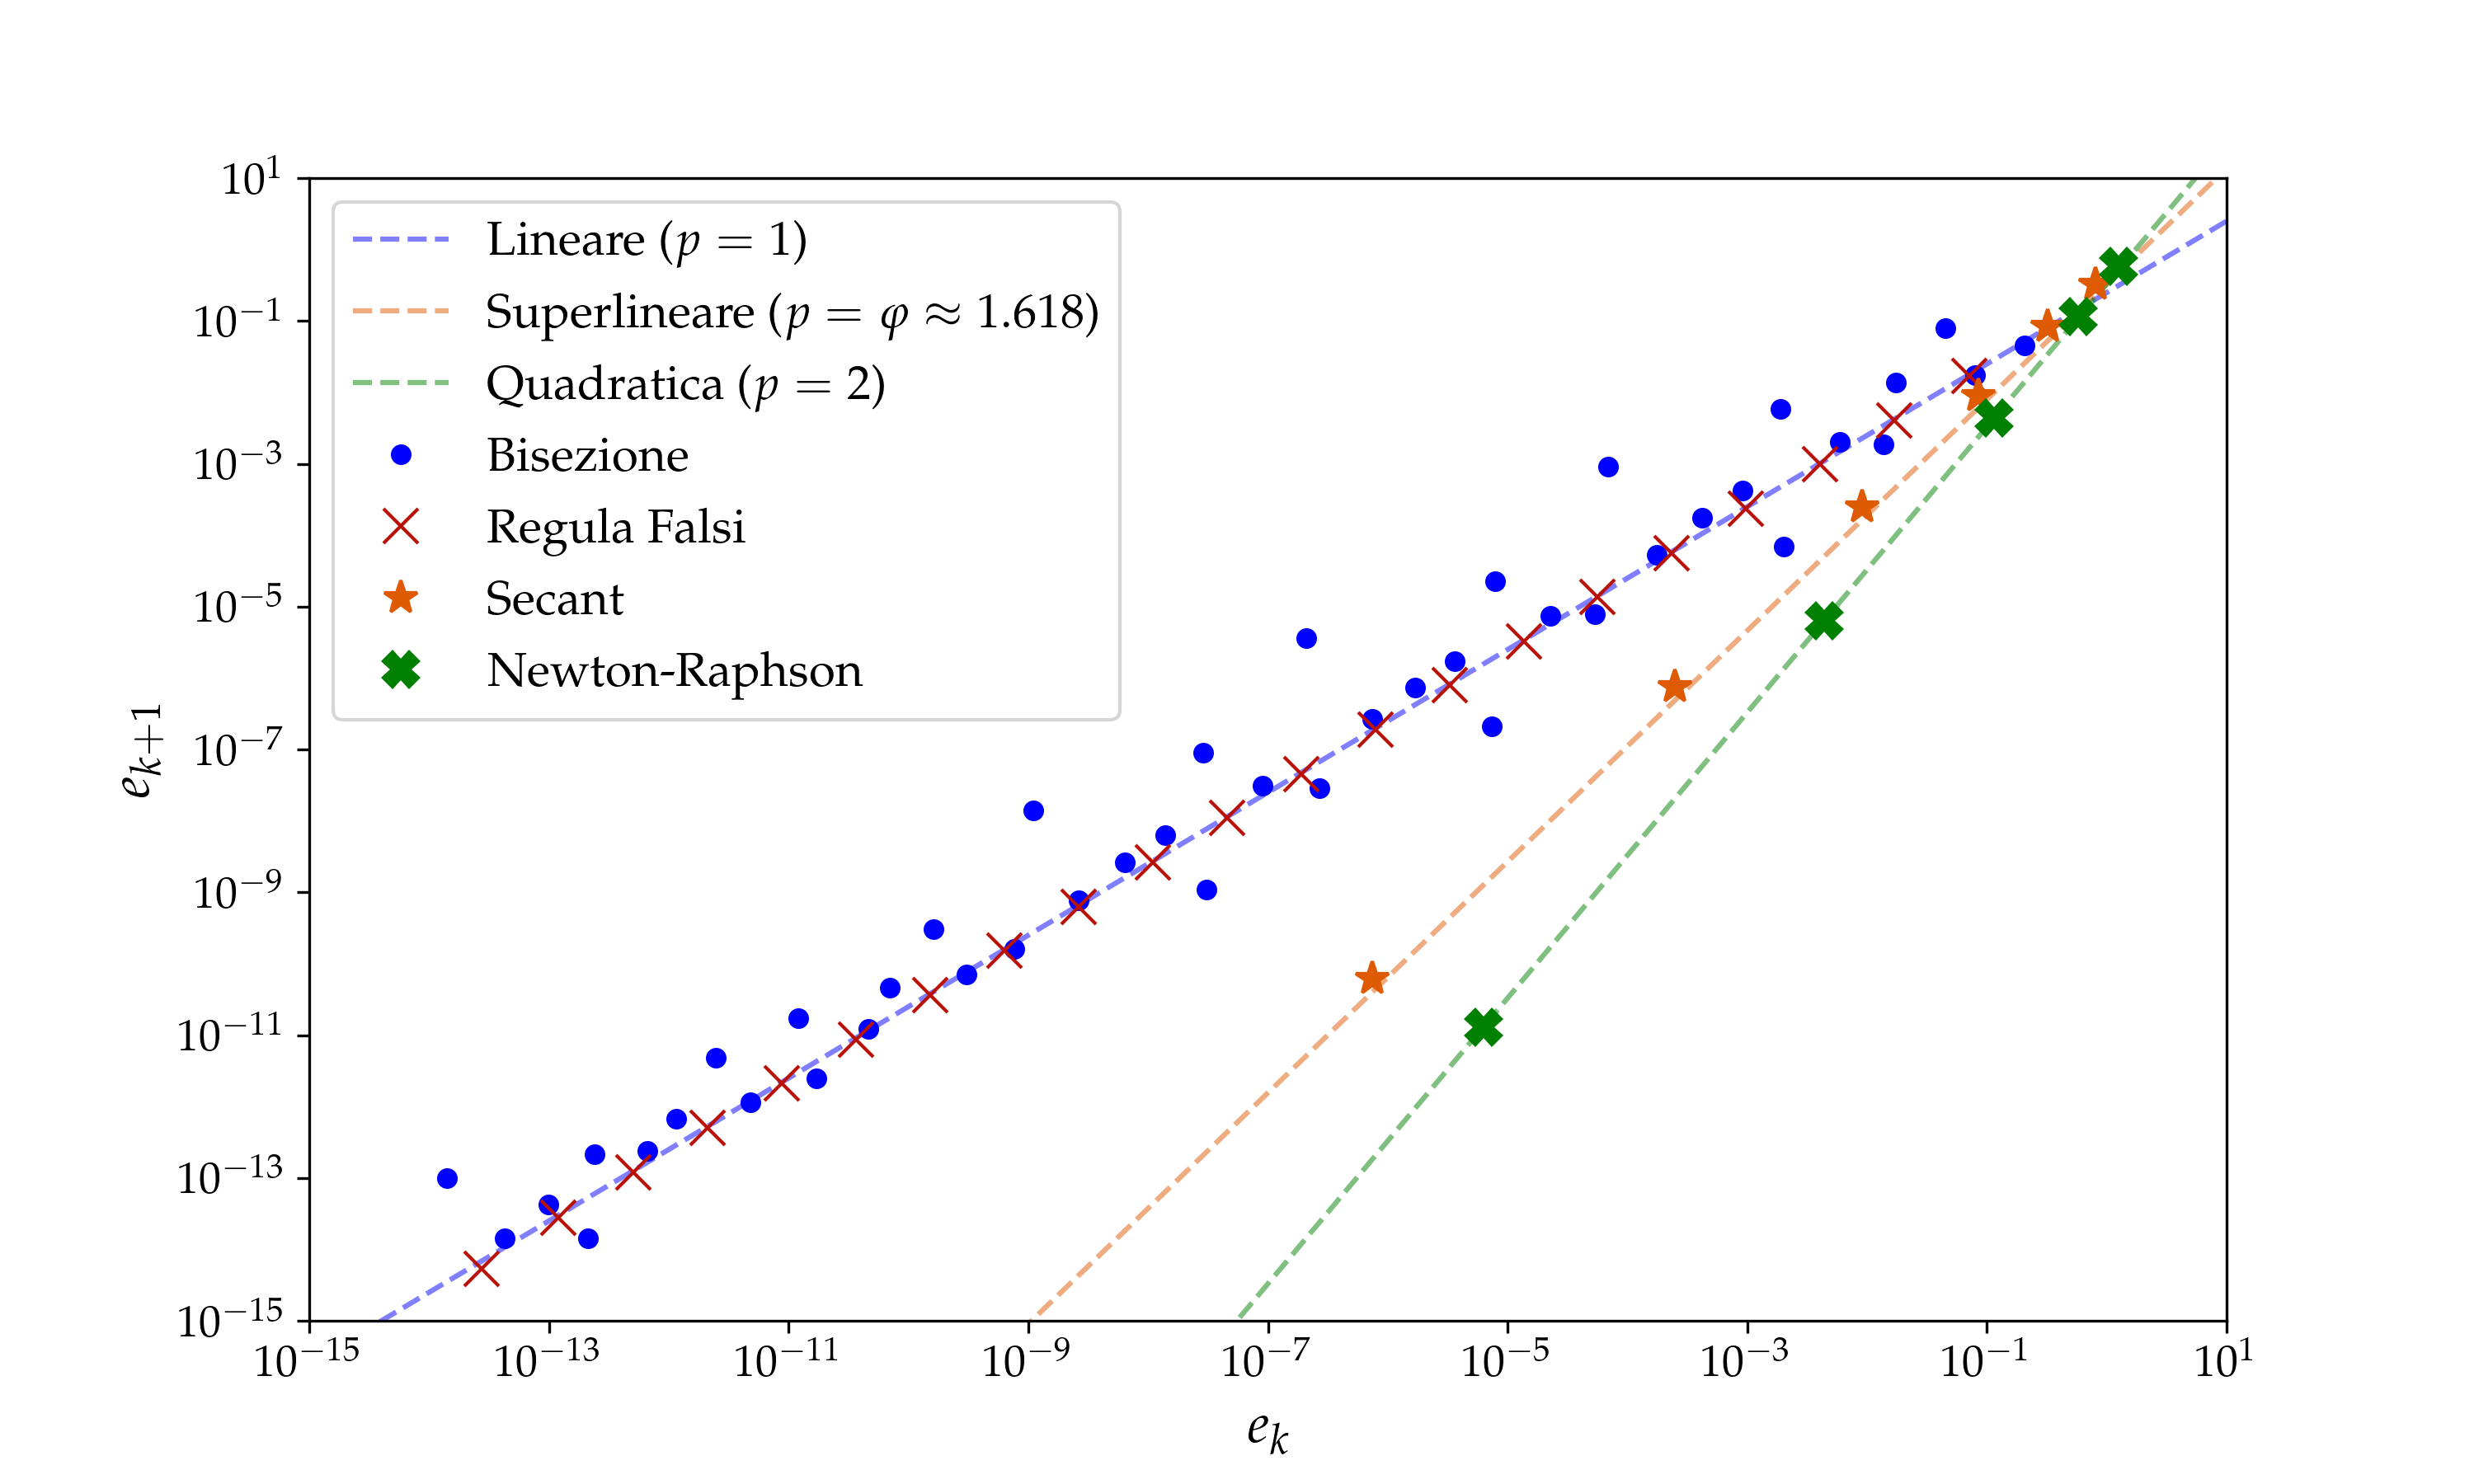
\includegraphics[width=0.95\linewidth]{images/14/scat_lines_even.png}
    \caption{l'andamento della convergenza unificato in un unico plot per tutti gli algoritmi. Tratteggiate le rette che segnano gli andamenti asintotici previsti e su cui, rispettivamente, si appoggiano i metodi. Per l'intestazione degli assi vale la stessa approssimazione di Fig.\ref{fig: fit Bis}.}
    \label{fig: confr even}
\end{figure}

\begin{figure}[H]
    \centering
    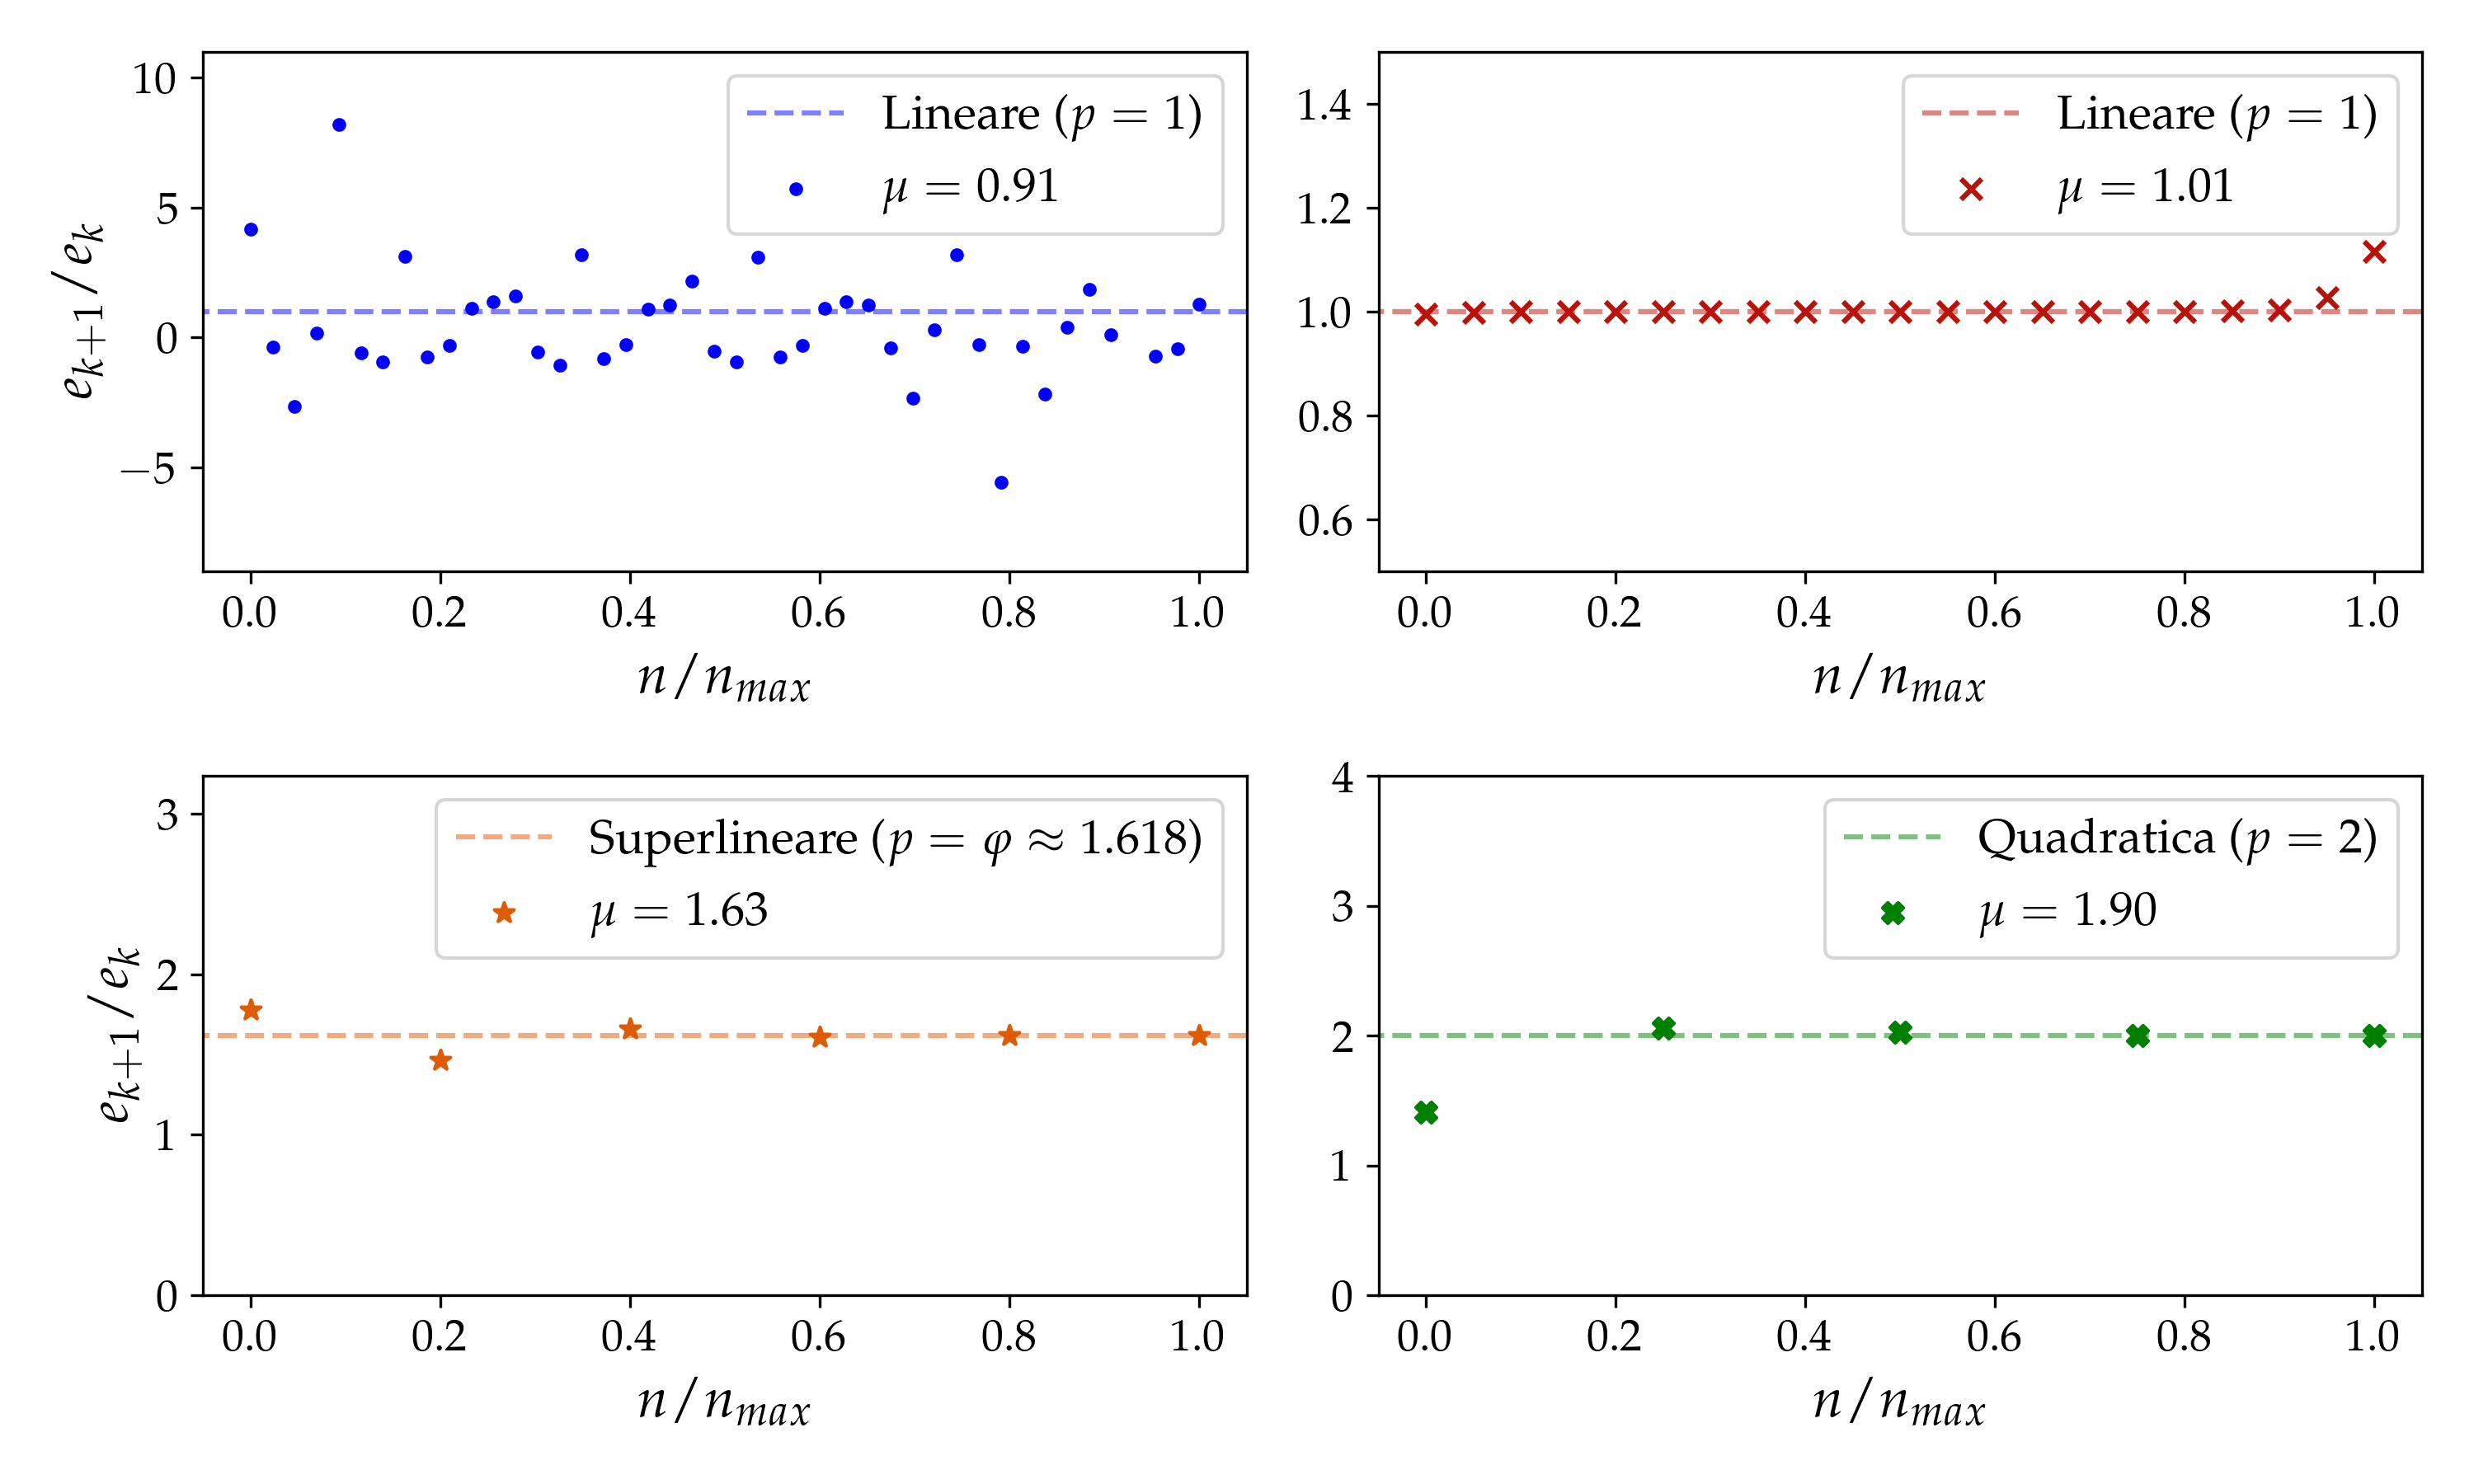
\includegraphics[width=0.9\linewidth]{images/14/single_scat_even.png}
    \caption{Nell'immagine sono separati i diversi andamenti dei punti organizzati nei plot in maniera da evidenziare l'aderenza proprio al $p$, fattore di scaling, aspettato. Sull'asse delle ascisse si leggono le iterazioni, normalizzate in maniera che sia uniforme la visualizzazione a prescindere della velocità di convergenza del singolo metodo. Sulle ordinate il rapporto $e_{n+1}/e_n$, che corrisponde al coefficiente angolare della retta nella Fig. \ref{fig: confr even} e che vediamo globalmente aderente al valore atteso. Viene indicato con $\mu$ il valore medio delle ordinate.}
    \label{fig: even mean}
\end{figure}


\begin{multicols}{2}
\begin{figure}[H]
    \centering
    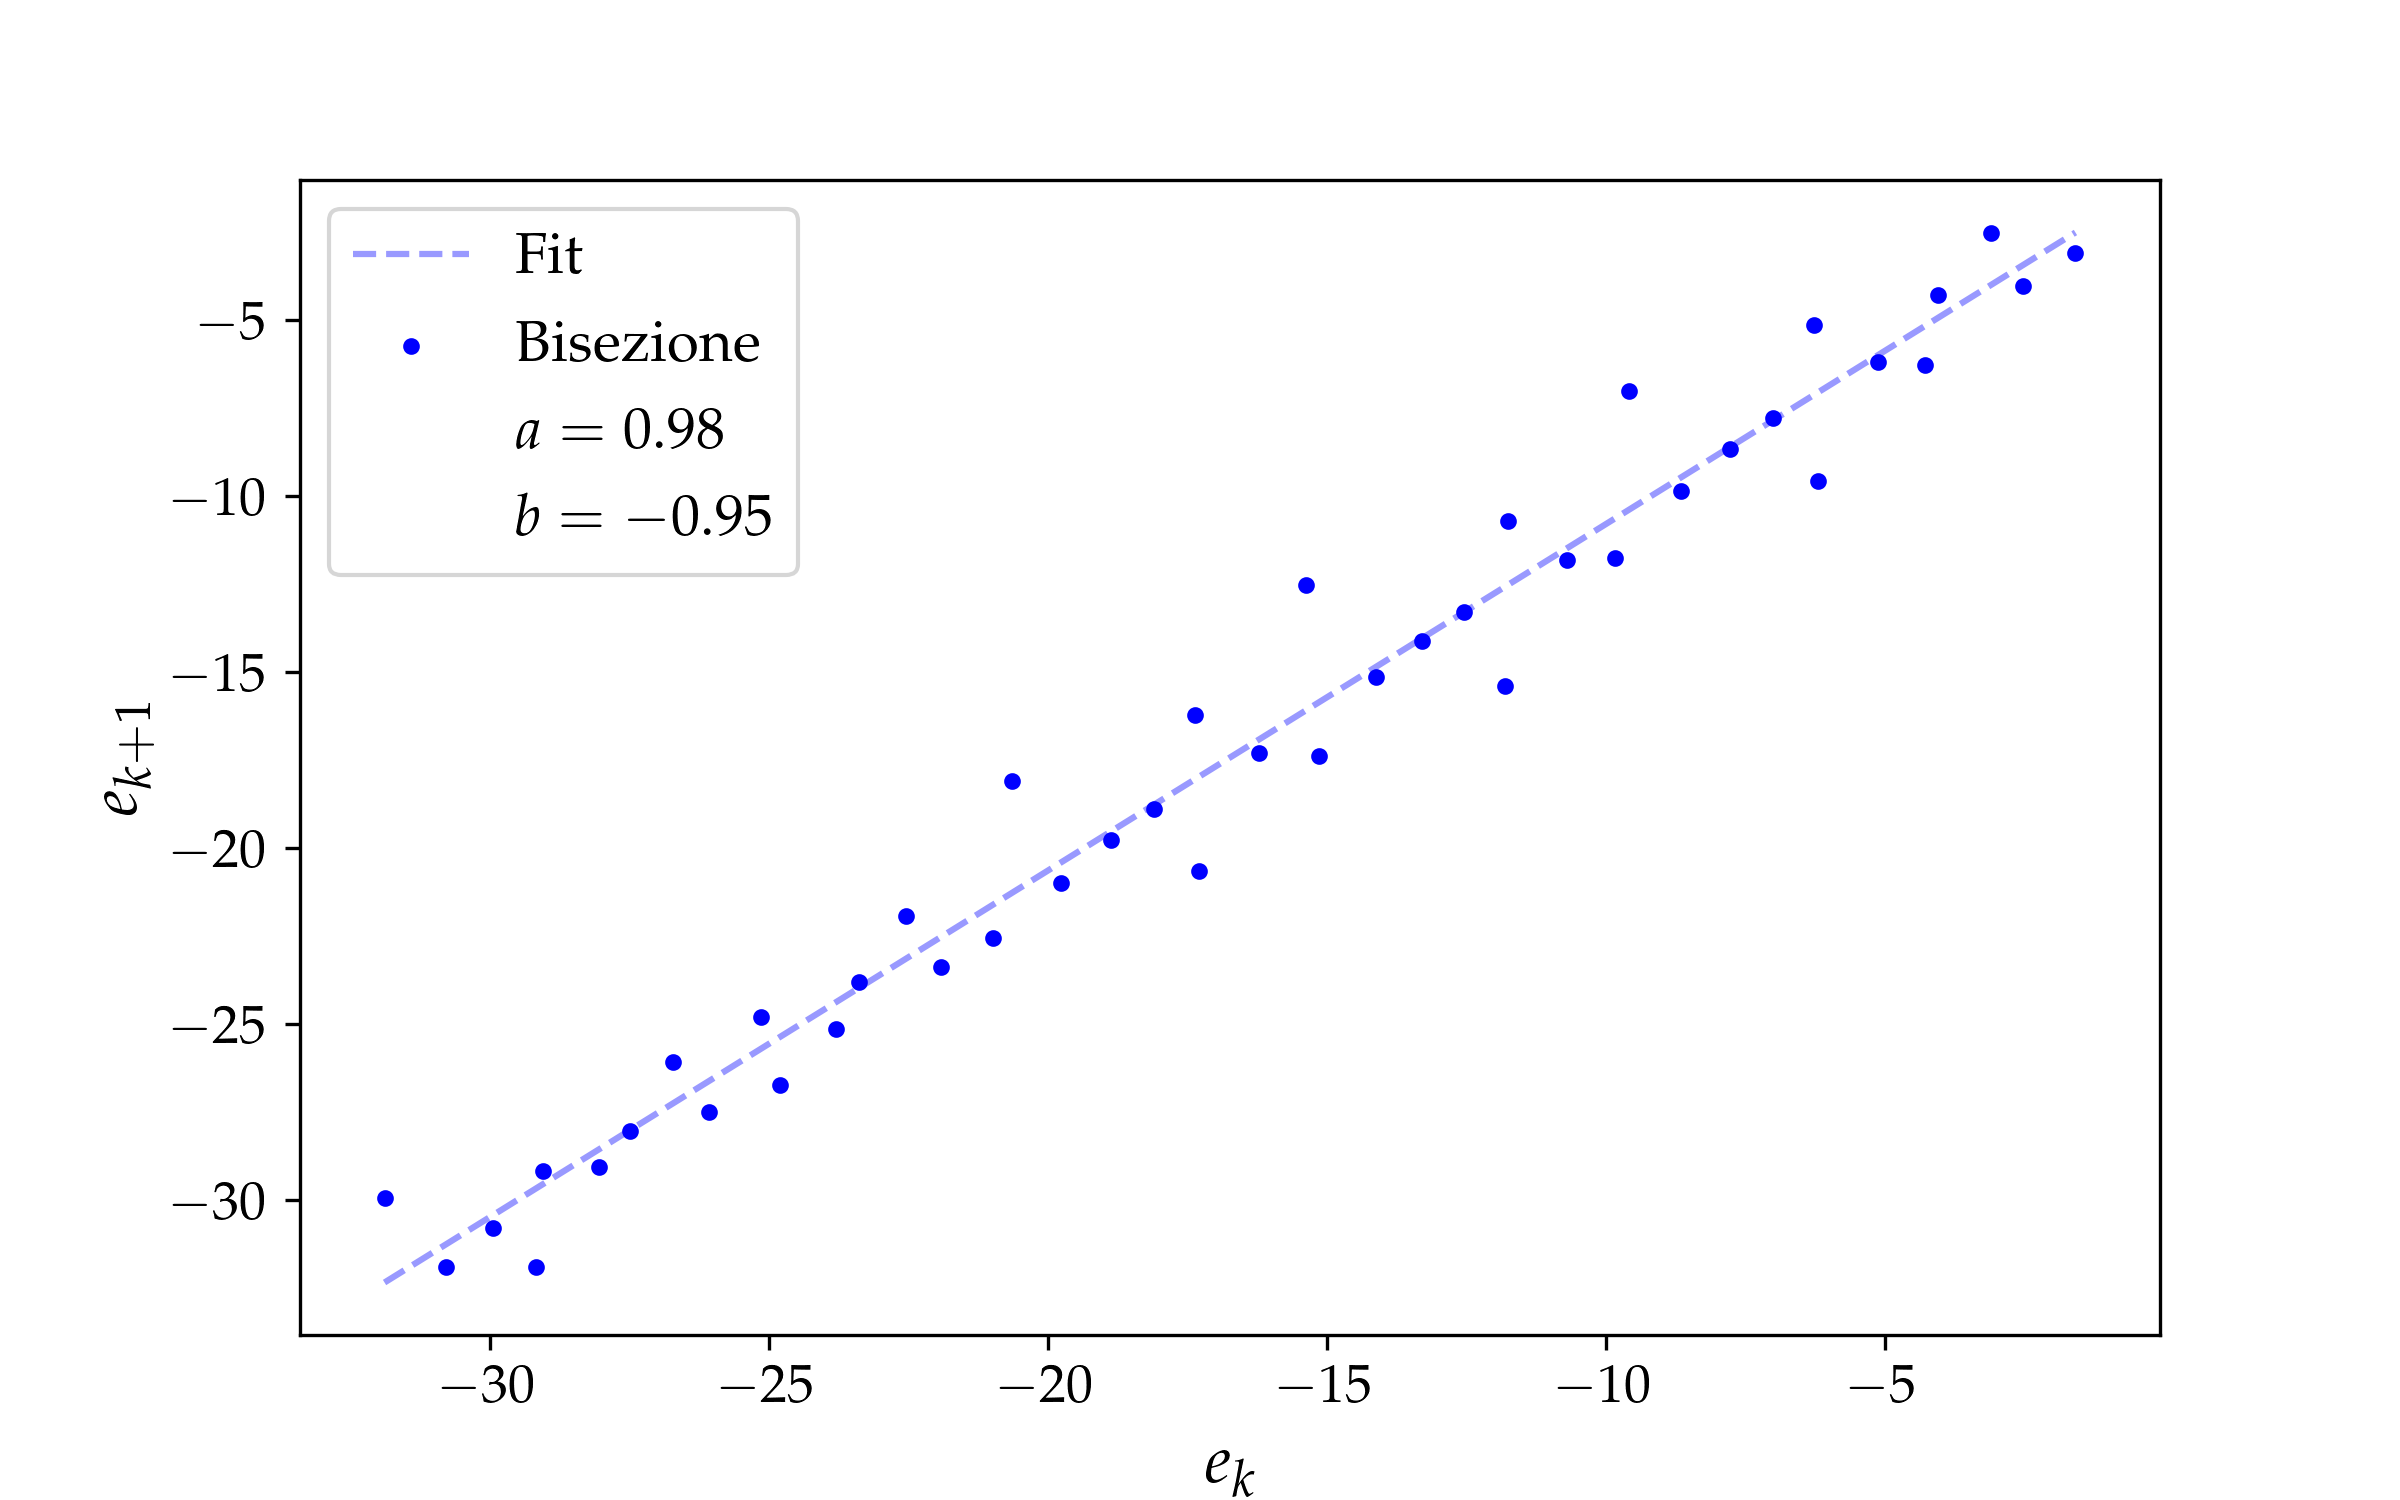
\includegraphics[width=\linewidth]{images/14/fit_Bisezione.png}
    \caption{Fit delle iterazioni di Bisezione per stima del parametro di scaling.}
    \label{fig: bisezione_fit}
\end{figure}

\begin{figure}[H]
    \centering
    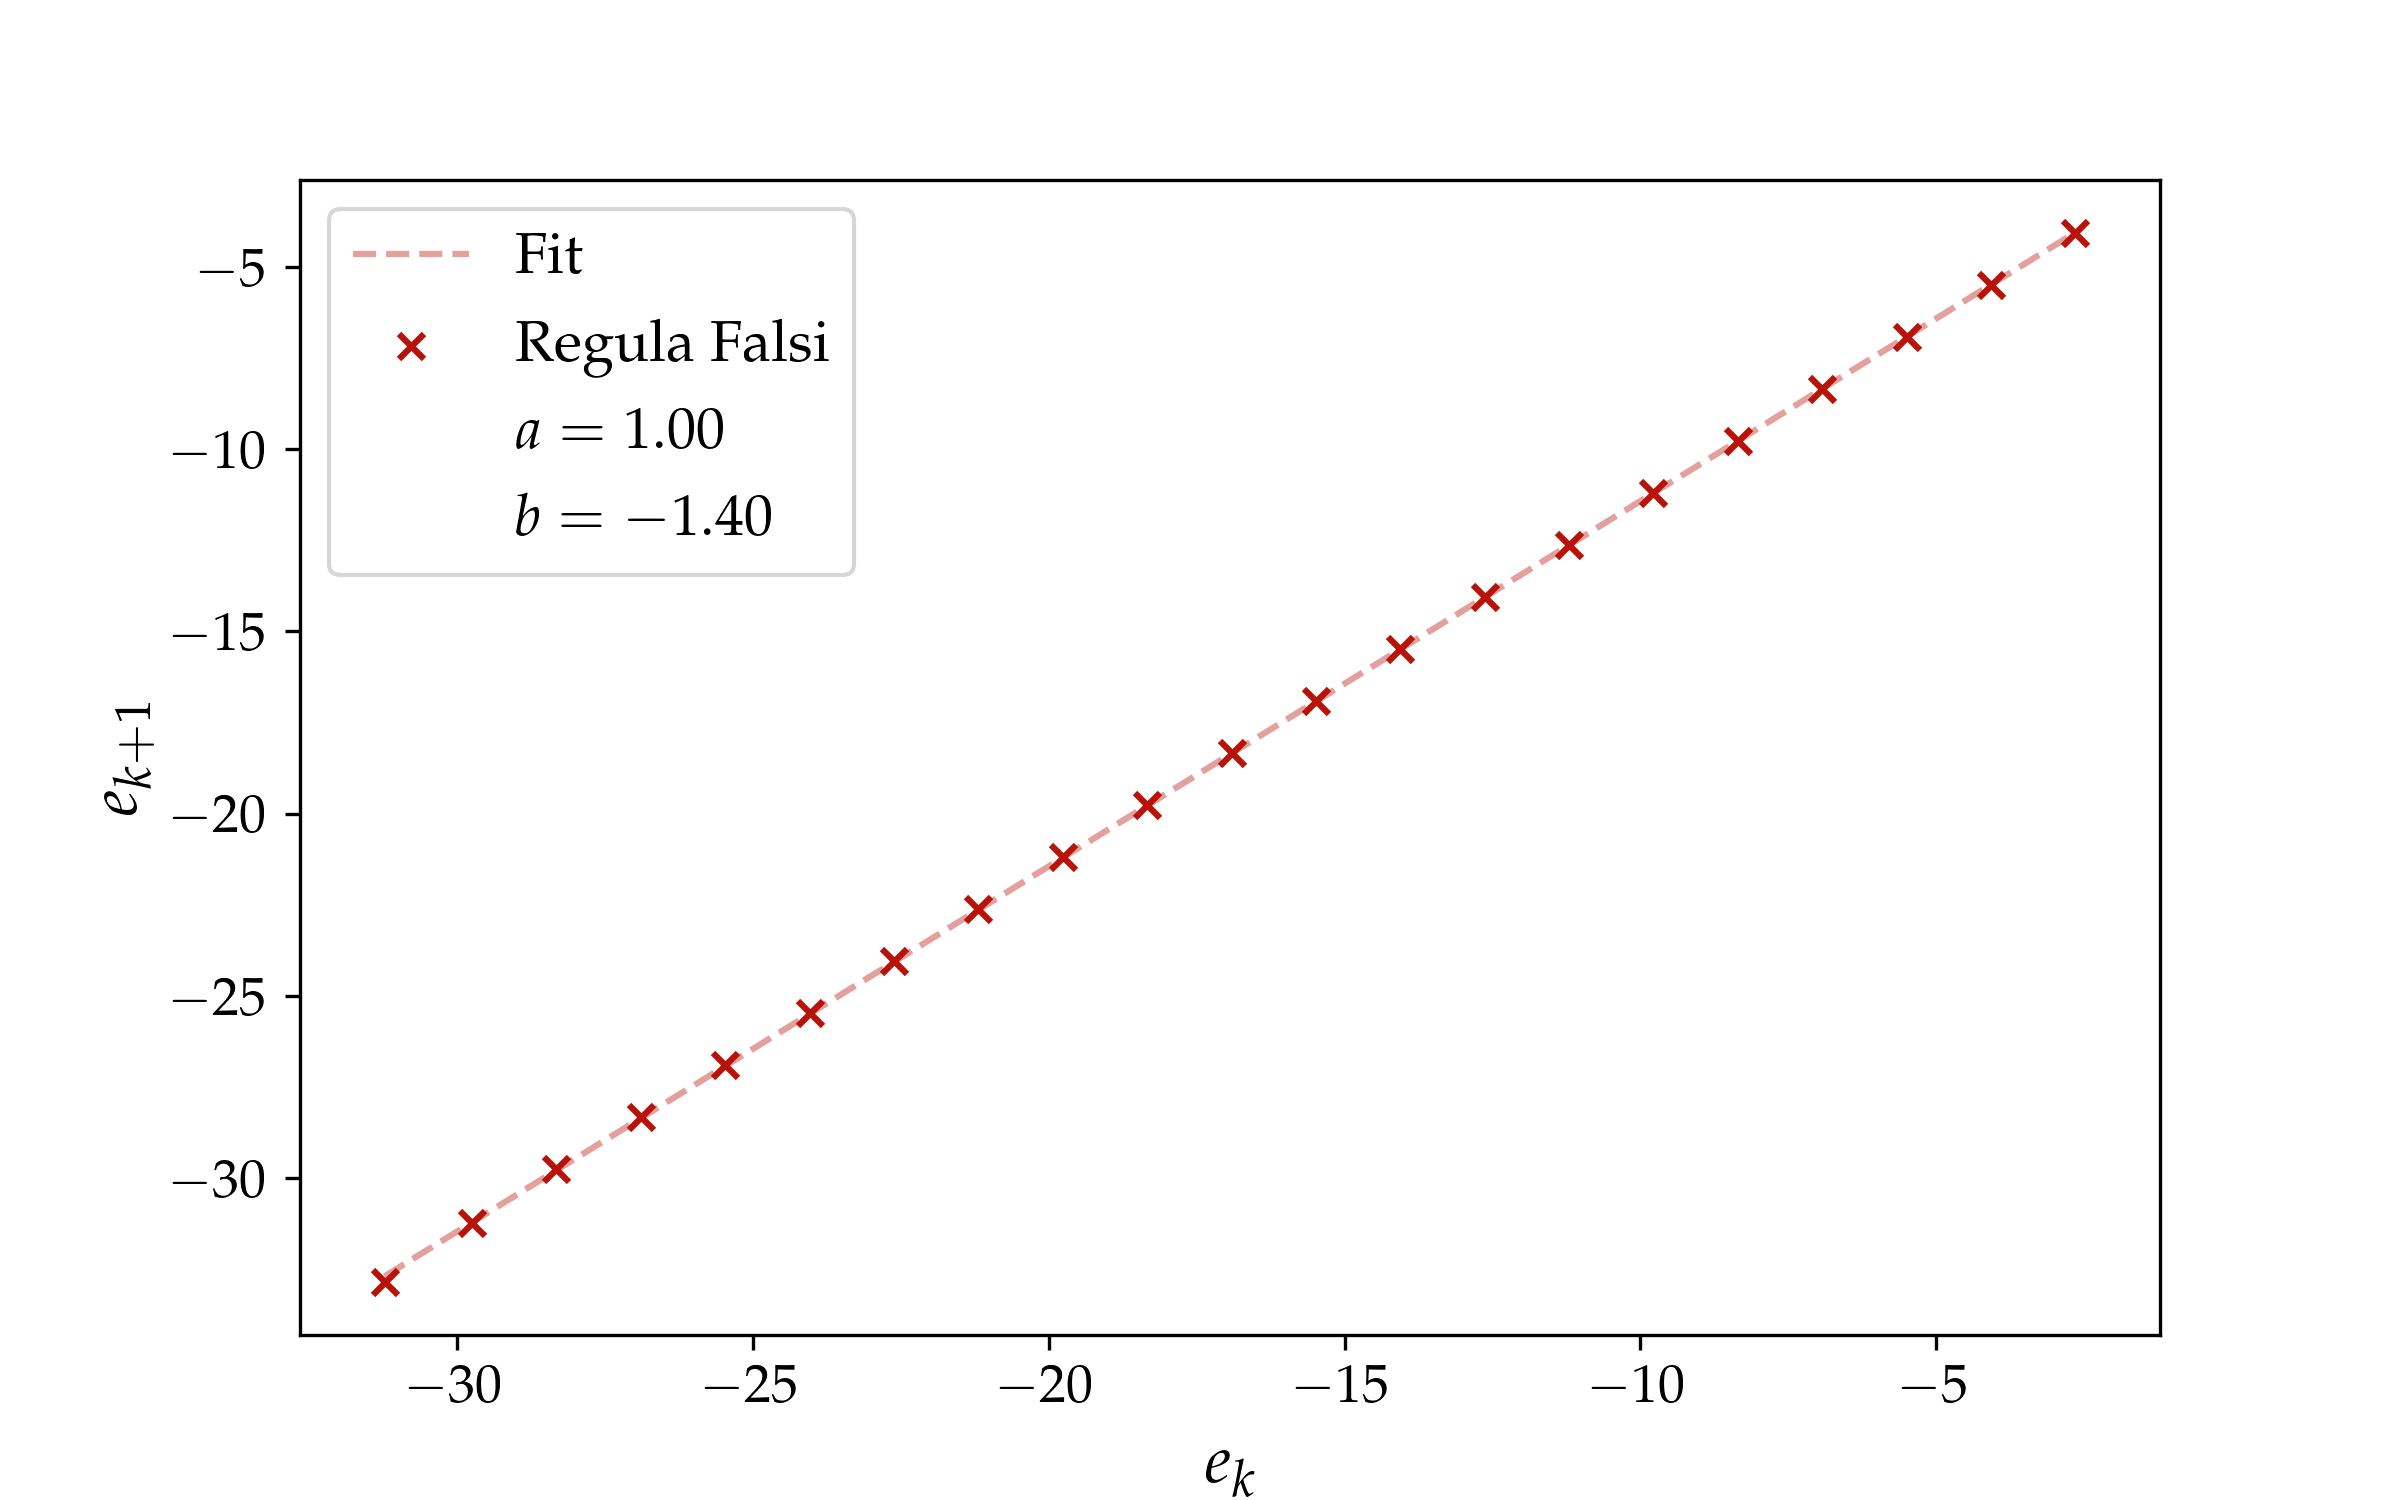
\includegraphics[width=\linewidth]{images/14/fit_Regula Falsi.png}
    \caption{Fit delle iterazioni di Regula Falsi per stima del parametro di scaling.}
    \label{fig: reg_fit}
\end{figure}
\end{multicols}

\begin{multicols}{2}
\begin{figure}[H]
    \centering
    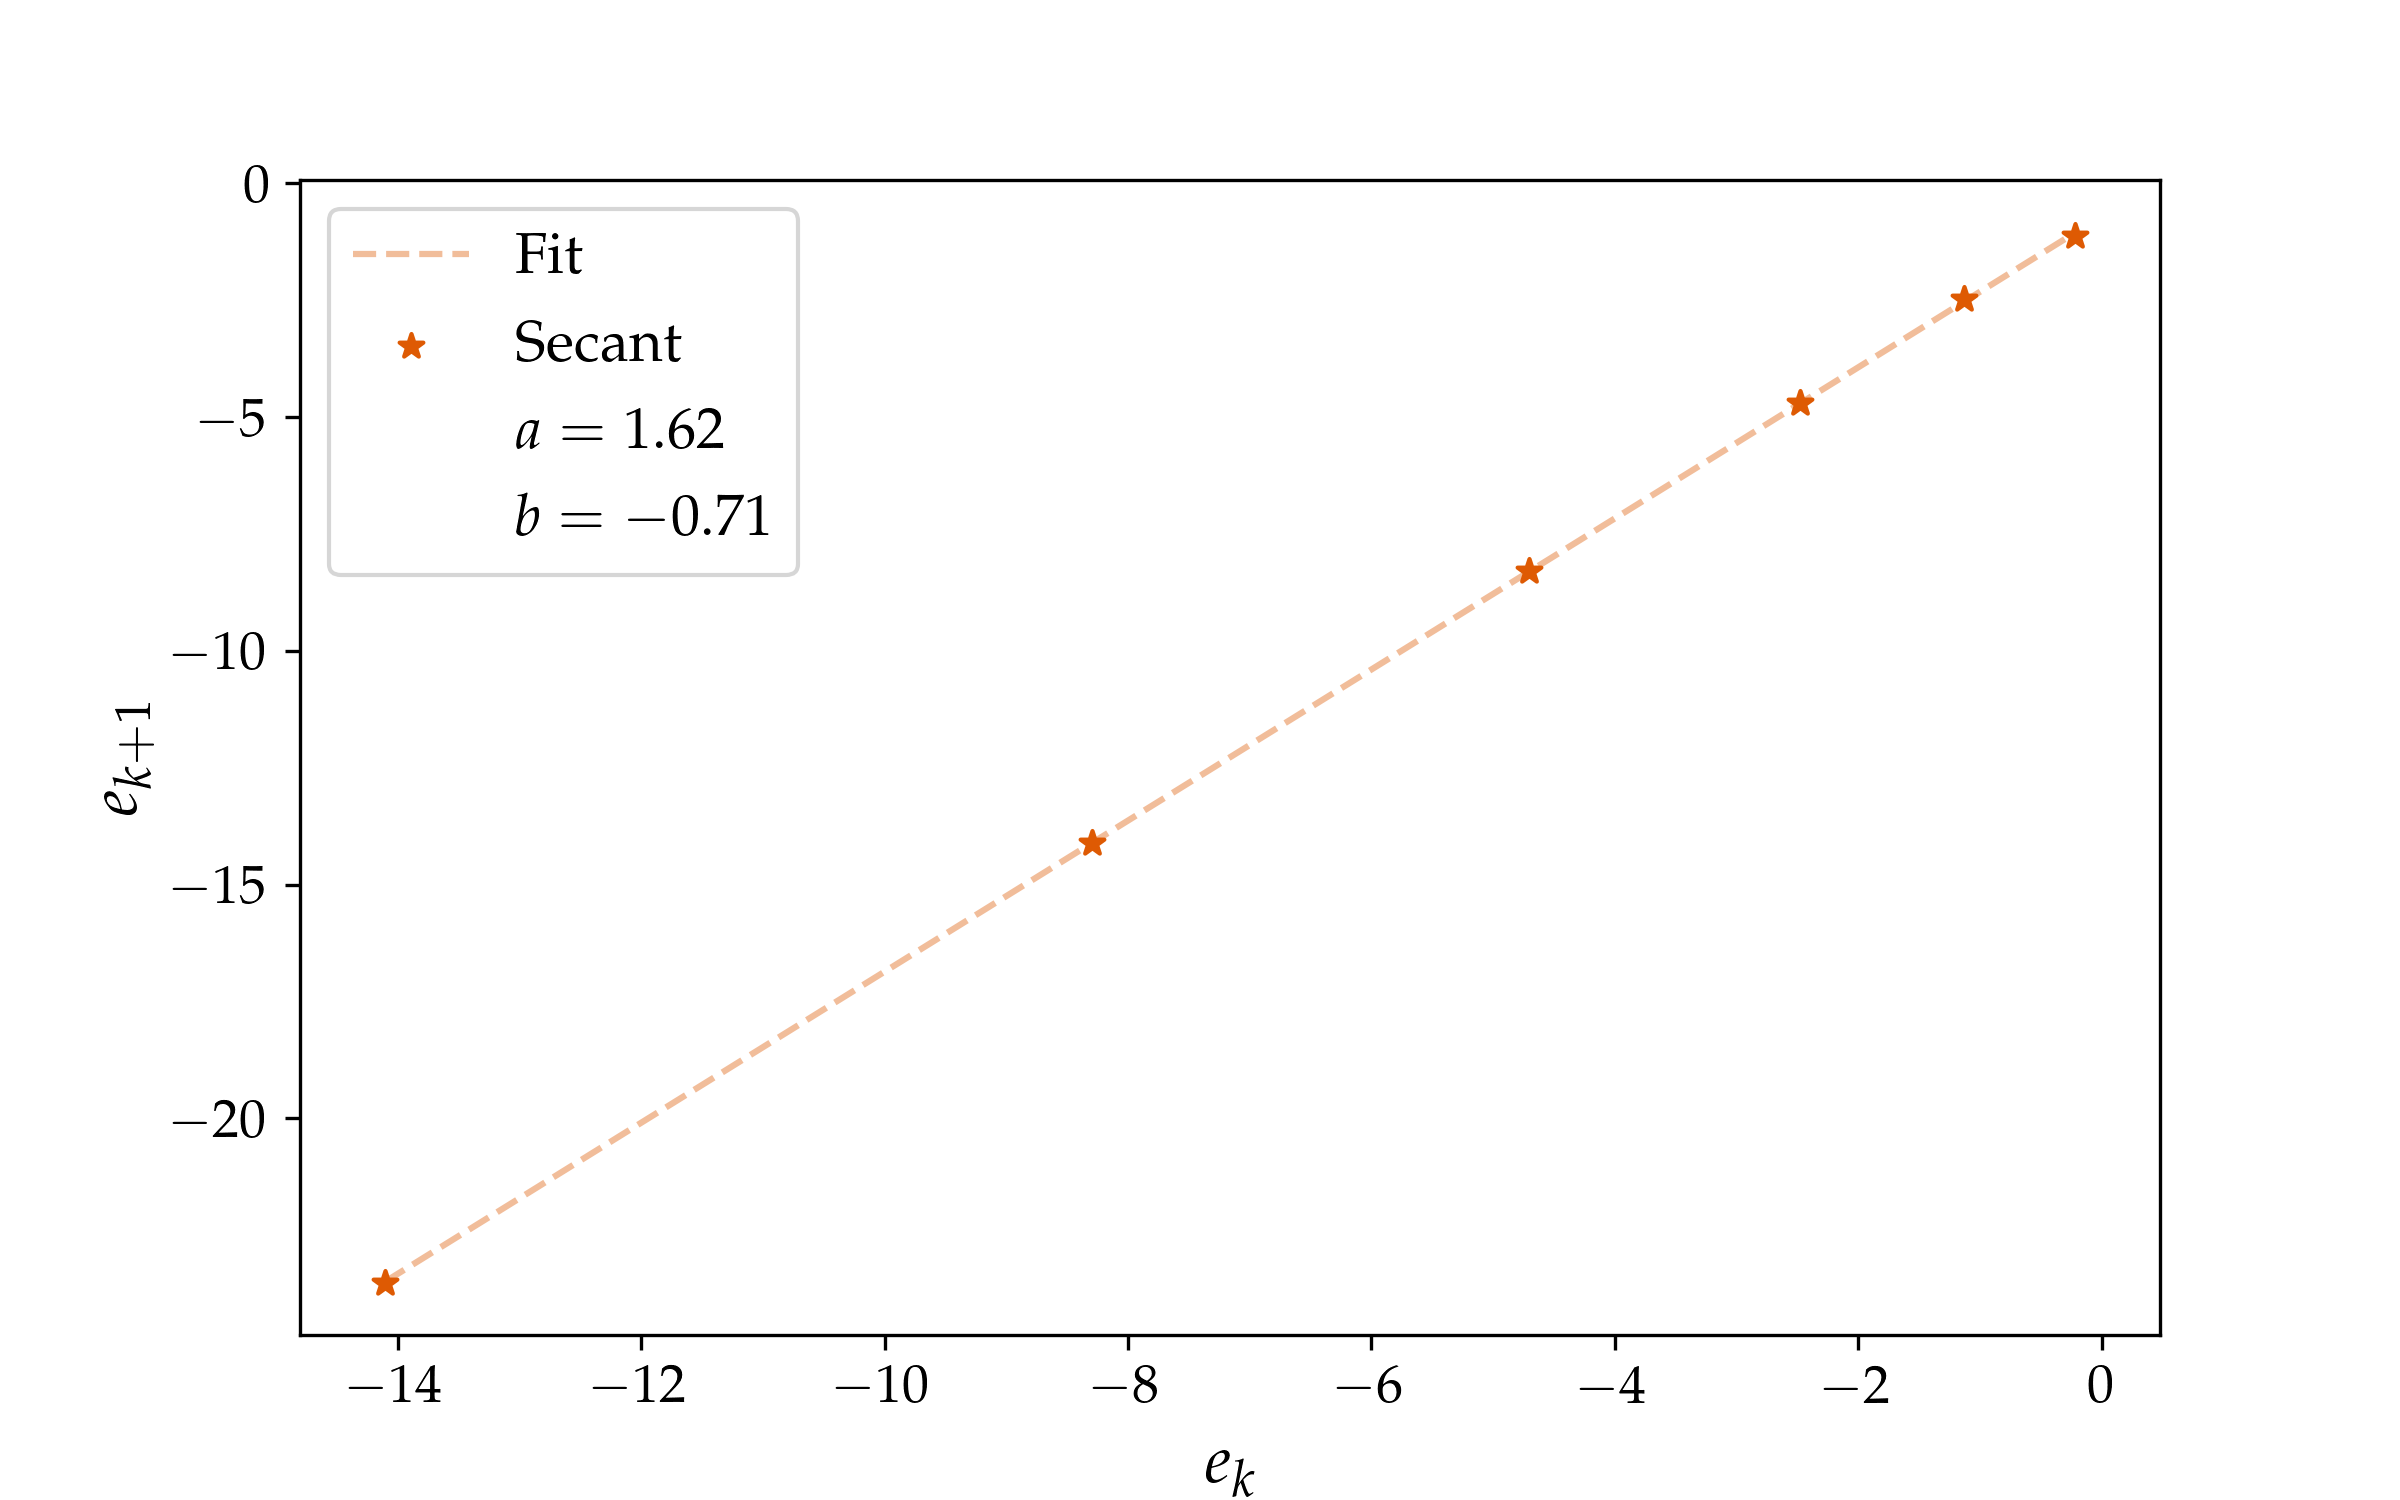
\includegraphics[width=\linewidth]{images/14/fit_Secant.png}
    \caption{Fit delle iterazioni di Secanti per stima del parametro di scaling.}
    \label{fig: sec_fit}
\end{figure}

\begin{figure}[H]
    \centering
    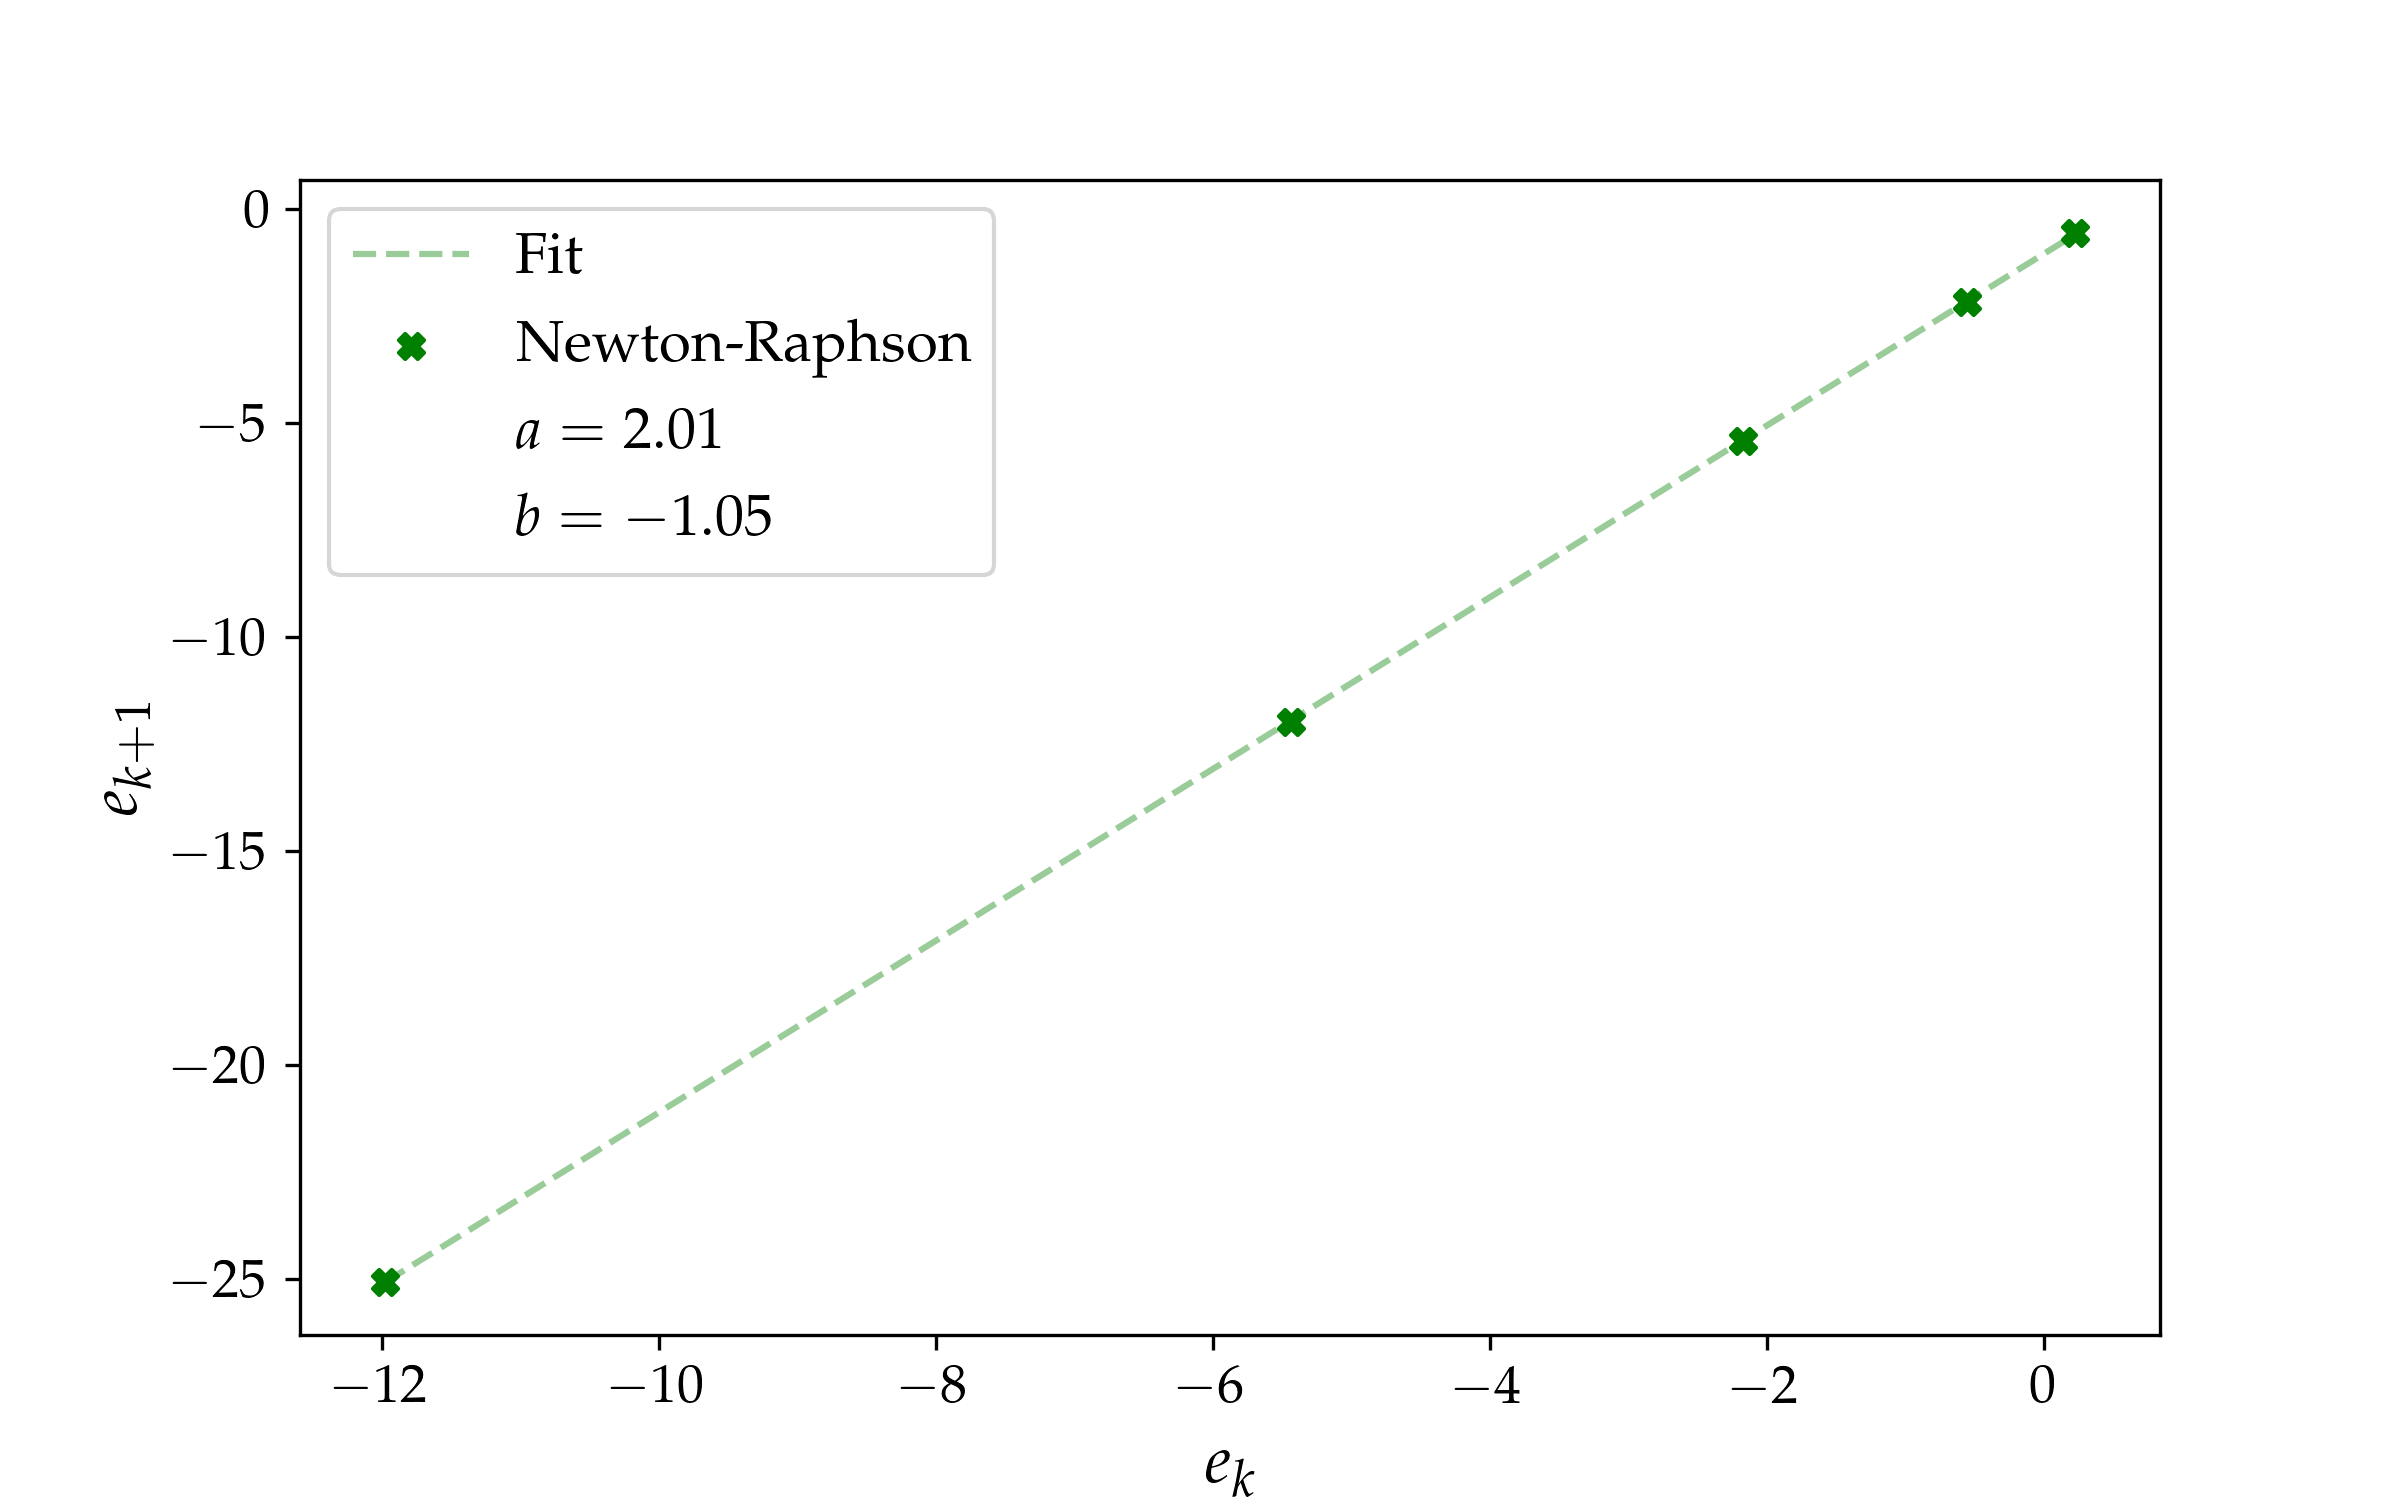
\includegraphics[width=\linewidth]{images/14/fit_Newton-Raphson.png}
    \caption{Fit delle iterazioni di Newton-Raphson per stima del parametro di scaling.}
    \label{fig: NR_fit}
\end{figure}

\end{multicols}

Le previsioni teoriche sui differenti rate di convergenza vengono quindi confermate dai fit.

\bigskip\noindent
Un ultima indagine è quella che si propone nel contesto della convergenza di N-R: si studia la storia dell'algoritmo in funzione dello \textit{starting point} $x_0 \in [-5.2,-5.0]$, campionando quattro punti in questo intervallo.\\
In Fig. \ref{fig: cn_fail} vediamo come la radice converga al valore approssimativo di $c_{true}\approx - 7.71$, tranne per il caso di $x_0=-5.0$: in questo caso l'algoritmo passa all'essere divergente, aumentando l'errore ad ogni step. 

\begin{elegantcode}
f(-5.07) = 13432.21
df(-5.07) = 9148811.79

f(-5.00) = -308.91
df(-5.00) = 4644.23
\end{elegantcode}

\noindent Il confronto con la Fig. \ref{fig: f even} chiarisce che sul lato sinistro della singolarità, che si trova molto vicina al punto $x=-5$ , la funzione è positiva per $x > 7.71$, mentre ha cambiato segno per $x=-5$, indicazione che ci siamo spostati sul lato destro del punto di discontinuità, ma con stesso segno della derivata. L'utilizzo della retta tangente per trovare la radice ci porterà solamente ad allontanarci ancora di più dalla radice vera, portando inevitabilmente alla divergenza del metodo così impostato.\\
In Fig. \ref{fig: errn_fail} un secondo plot che evidenzia invece l'errore relativo alla radice n-esima, confrontando la \textit{guess} con la migliore stima, che viene fatta trovando lo zero con N-R e $x_0=-7.0$.



\begin{figure}[H]
    \centering
    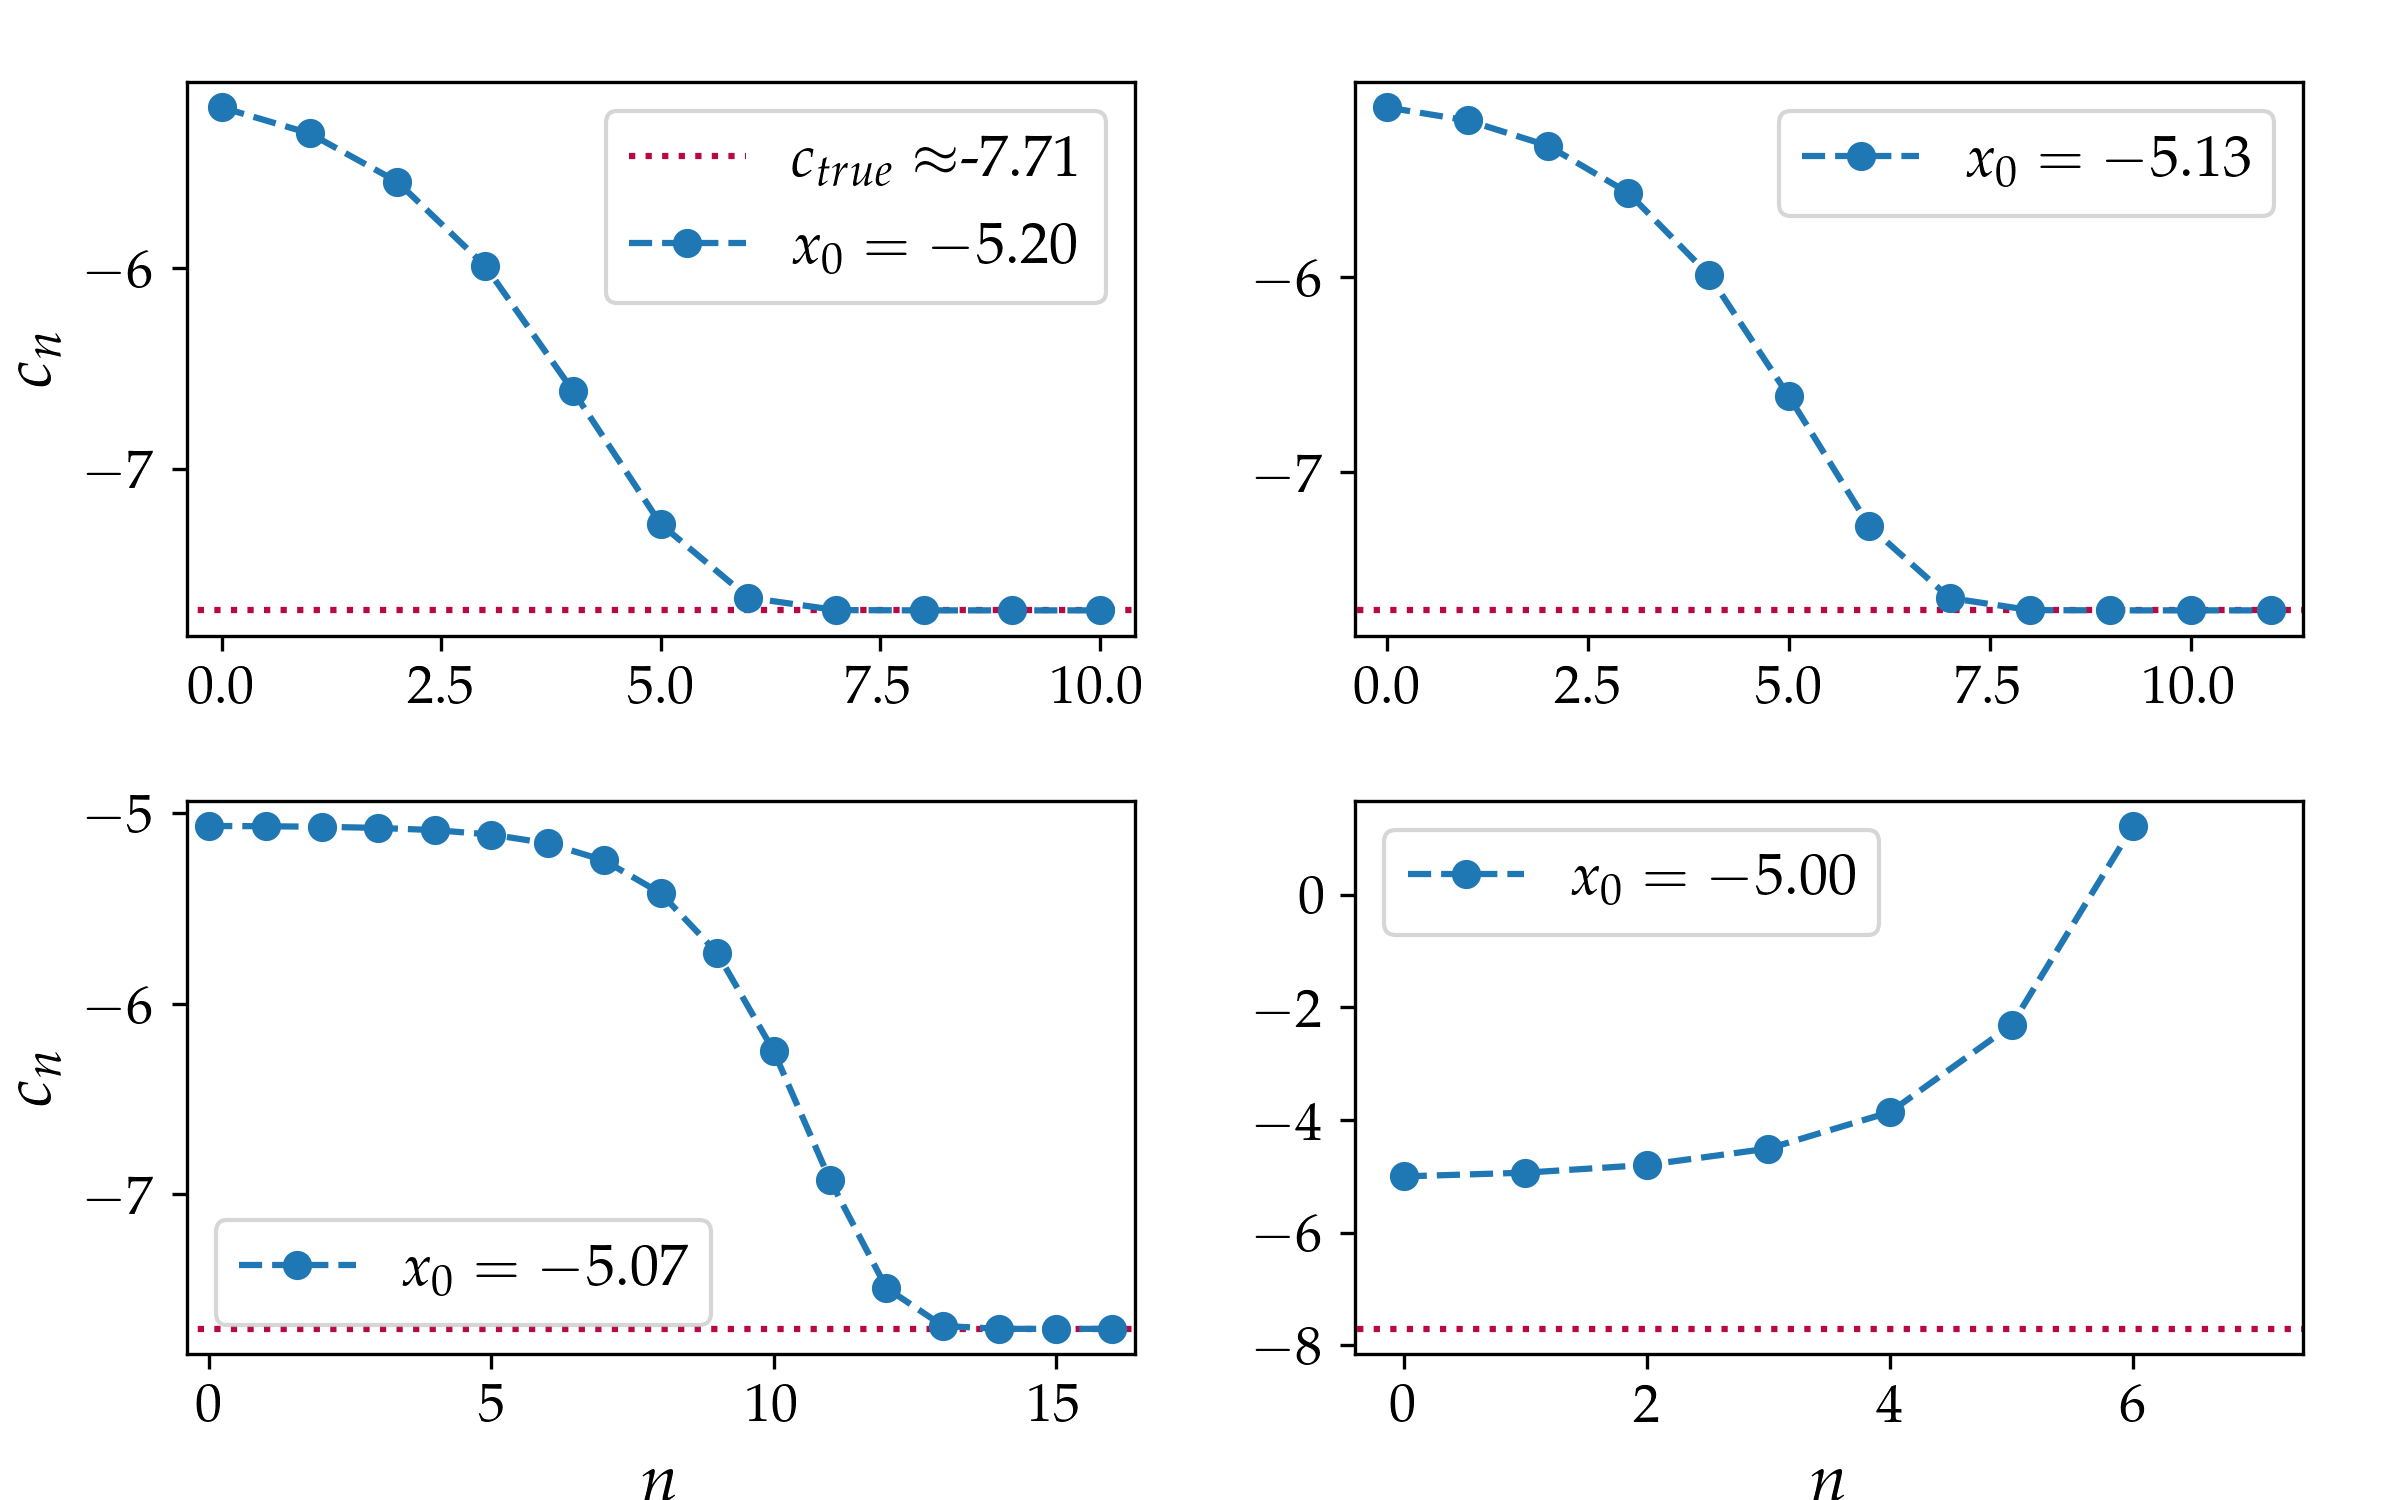
\includegraphics[width=0.8\linewidth]{images/14/cn_fail.png}
    \caption{La storia della radice n-esima di N-R al variare dello \textit{starting point} $x_0$.}
    \label{fig: cn_fail}
\end{figure}
\begin{figure}[H]
    \centering
    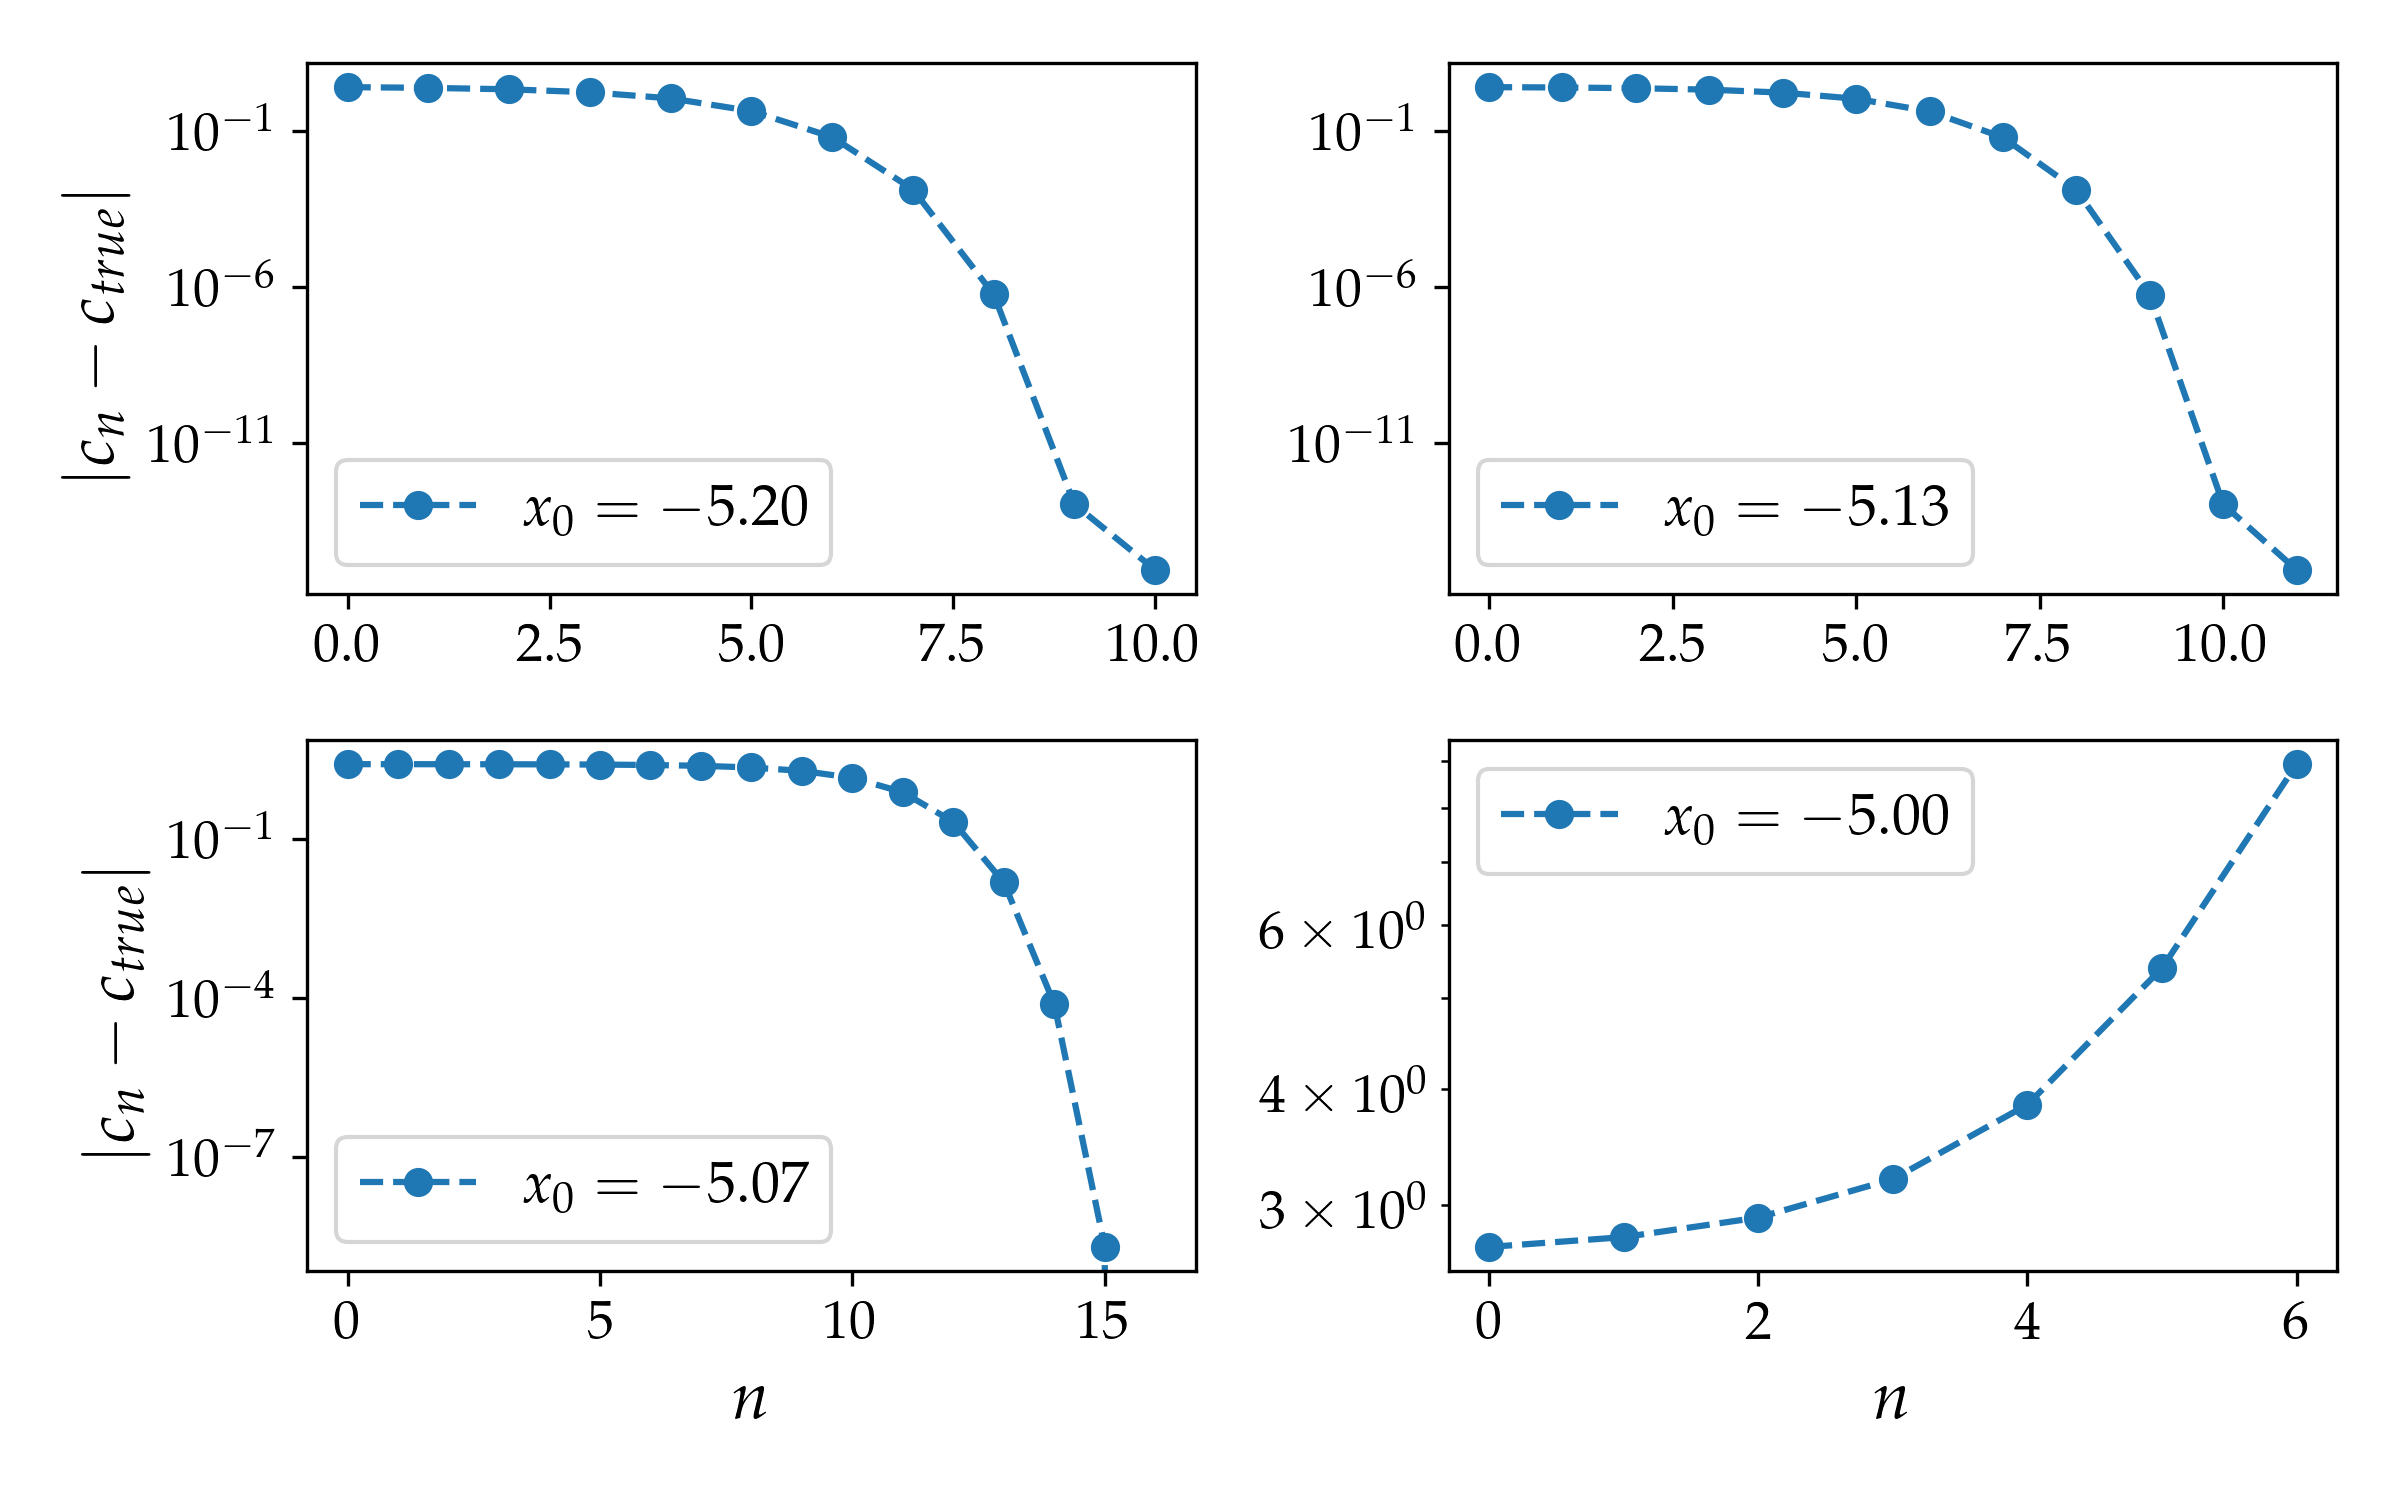
\includegraphics[width=0.8\linewidth]{images/14/errn_fail.png}
    \caption{La storia dell'errore sulla radice n-esima di N-R al variare dello \textit{starting point} $x_0$.}
    \label{fig: errn_fail}
\end{figure}

\newpage

Infine vogliamo studiare l'analogo caso per gli stati dispari:
\[
f(E) =k(E) \cot\left(\frac{k(E) L}{2}\right) + \bar\kappa(E)
\]

Il plot della funzione è necessario per avere un'idea di dove inizializzare la ricerca dello zero.

\begin{figure}[H]
    \centering
    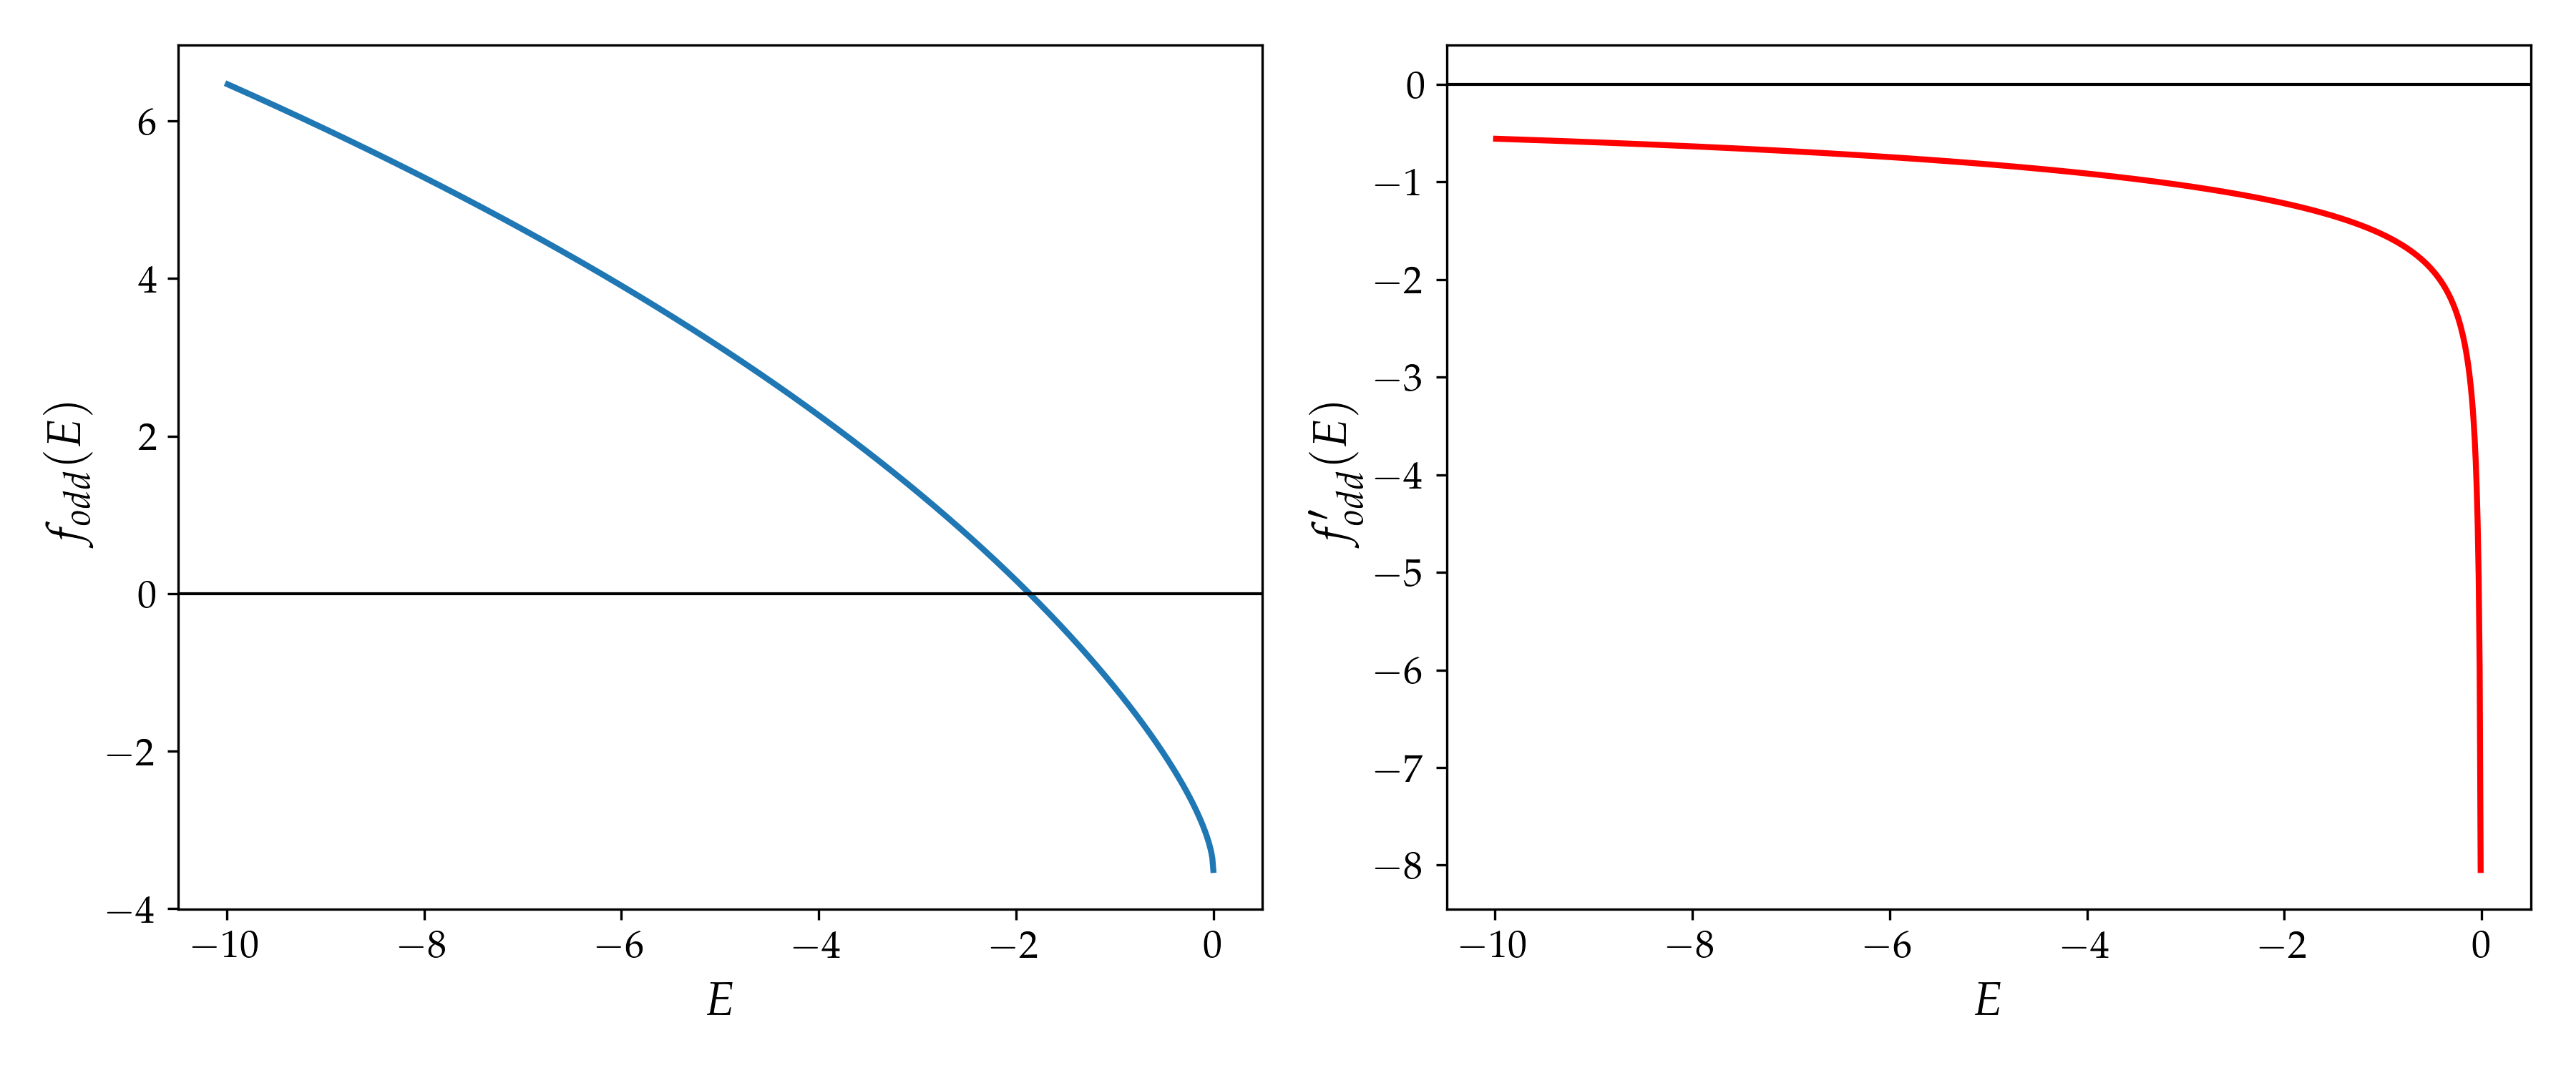
\includegraphics[width=\linewidth]{images/14/f_odd.png}
    \caption{Plot della funzione dispari e della sua derivata: nel dominio aperto mostrato non sono presenti singolarità e la funzione appare continua e derivabile.}
\end{figure}

I diversi metodi restituiscono i seguenti risultati:
\begin{elegantcode}
Bisection        c = -1.8628522388353397
                 iters = 46

Regula Falsi     c = -1.862852238835343
                 iters = 19

Secant           c = -1.86285223883534
                 iters = 6

Newton-Raphson   c = -1.8628522388353397
                 iters = 7
\end{elegantcode}


\bigskip\noindent Diamo quindi l'ultima descrizione del problema presentando i risultati finali per le due energie riferite agli stati legati con parità opposta, scegliendo come valori di riferimento numerici rispettivamente i due calcolati con il metodo di Newton-Raphson:
\begin{align*}
E_{\text{pari}} &= -7.705009250739082\\
E_{\text{dispari}} &= -1.8628522388353397
\end{align*}

\begin{figure}[H]
    \centering
    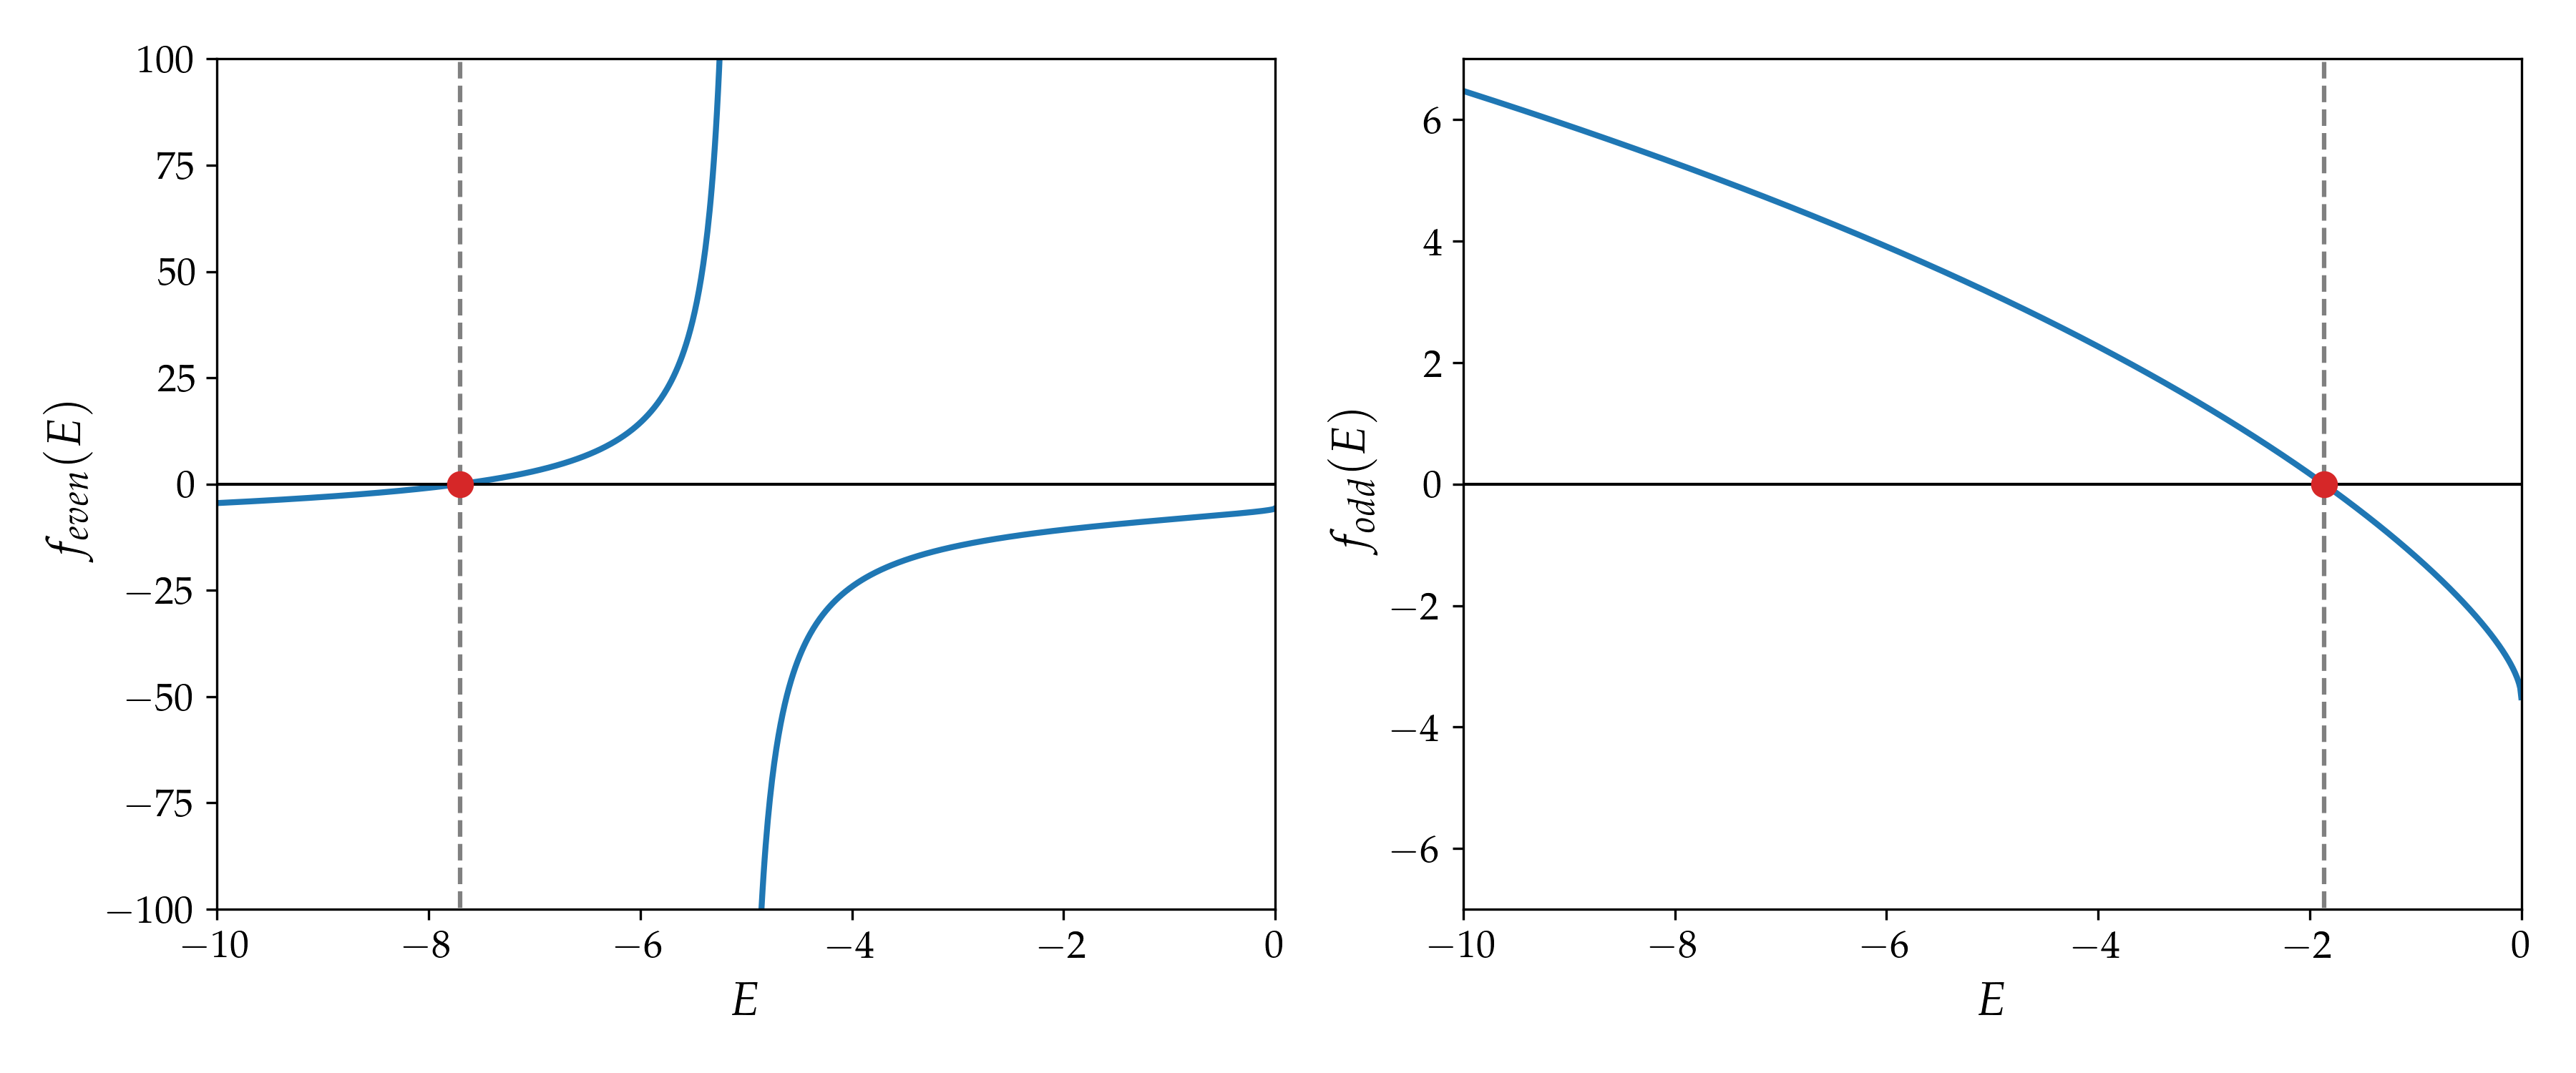
\includegraphics[width=\linewidth]{images/14/tot_f_plot.png}
    \caption{Rappresentazione delle due funzioni e degli zeri individuati con metodo di N-R.}
    \label{fig:placeholder}
\end{figure}


\newpage


\section{Esercizio 5.4.1}
\subsection{Problem Statement}

Scrivi un programma che, dato un polinomio, trovi le sue radici utilizzando la ricerca di autovalori discusso nella Sezione \textit{Problemi agli autovalori} e ne verifichi la correttezza. Si noti che il polinomio è completamente specificato dai coefficienti nella base monomiale. Scrivi il metodo di ricerca delle radici in modo modulare e applicalo ai seguenti casi:

\begin{enumerate}
    \item Il polinomio di Legendre di ordine 10
    \[
    \frac{1}{256}(46189x^{10} - 109395x^8 + 90090x^6 - 30030x^4 + 3465x^2 - 63)
    \]
    
    \item Il polinomio di Hermite di ordine 6
    \[
    H_6(x) = 64x^6 - 480x^4 + 720x^2 - 120
    \]
    
    \item I polinomi di Hermite soddisfano la relazione ricorsiva
    \[
    H_{n+1}(x) = 2xH_n(x) - 2nH_{n-1}(x), \quad H_0(x) = 1, H_{-1}(x) = 0
    \]
    Scrivi un programma che calcoli le radici del polinomio di Hermite di ordine $n$, $H_n(x)$. Costruisci il polinomio dalla relazione ricorsiva e verifica il risultato rispetto al compito precedente.
\end{enumerate}

Utilizza il risolutore di autovalori basato sulla decomposizione QR per questo esercizio.


\subsection{Premessa Teorica}
N-R si configura come un buon metodo, ma per il caso di una funzione con più radici esiste la possibilità che l'algoritmo converga su una  radice diversa da quella di nostro interesse. In più sarebbe interessante pensare di implementare un metodo che non debba ricercare i valori uno alla volta. In particolare ci occupiamo del caso in cui la funzione sia un polinomio di grado $n$, quindi con lo stesso numero di radici.\\

\medskip\noindent
Se definisco il polinomio
\[
    P_n(x) = c_0 + c_1 x + \dots + c_n x^n
\]

dividendo per $c_n$ e ridefinendo i $\bar c_i = c_i/c_n$:
\[
    P_n(x) = \bar c_0 + \bar c_1 x + \dots + x^n
\]

Introducendo la \textit{Companion matrix} $C_{ij}$:
\[
    C_{ij} = \begin{pmatrix} 
    0 & 1 & 0 & \dots & 0 & 0 \\
    0 & 0 & 1 & \dots & 0 & 0 \\
    \vdots & \vdots & \vdots & \vdots & \vdots & \vdots \\
    0 & 0 & 0 & \dots & 0 & 1\\
    -\bar c_0 & -\bar c_1 & -\bar c_2 & \dots & -\bar c_{n-2} & -\bar c_{n-1}
    \end{pmatrix}
\]

e il vettore $X_i(x) = (1,x,x^2 \dots x^{n-1})$, allora si può scrivere che:

\[
    \sum_j C_{ij} X_j(x) = \begin{pmatrix} x \\ x^2 \\ \cdots \\ -\bar c_0  -\bar c_1 x + \dots \end{pmatrix} = \begin{pmatrix} x \\ x^2 \\ \cdots \\ x^n - P_n(x) \end{pmatrix}
\]

Assumendo $P_n(x_0)=0$, cioè $x_0$ una radice del polinomio:
\[
    \sum_j C_{ij} X_j(x_0) = x_0 \begin{pmatrix} 1 \\ x_0 \\ \cdots \\ x_0^{n-1} \end{pmatrix} = x_0 X_i(x_0)
\]

\noindent Cioè $x_0$ è un autovalore di $C_{ij}$, con autovettore $X_i(x_0)$: abbiamo quindi la possibilità di implementare gli algoritmi dei capitoli precedenti per la ricerca di questi autovalori, e usando per esempio il \textit{QR eigensolver} possiamo trovarli tutti in una sola volta. La base che formano questi autovettori rappresenta i vettori riga della matrice di Vandermonde.

\subsection{Metodi Numerici e Algoritmi}
\subsubsection{Polinomi di Legendre di ordine 10}
Le radici estratte sono:
\begin{elegantcode}
Roots Legendre 10: [-0.97390653 -0.86506337 -0.67940957 -0.43339539 -0.14887434  0.14887434
  0.43339539  0.67940957  0.86506337  0.97390653]
\end{elegantcode}

\begin{multicols}{2}
    \noindent e la loro rappresentazione grafica in Fig. \ref{fig: Leg10}. Già dalla figura si può vedere come le radici che troviamo siano una buona approssimazione di quelle reali, ma lo confermiamo con una valutazione della funzione in questi punti ($|\text{Leg}_{10}(x_i)|\approx0$); si noti che l'algoritmo QR, di cui facciamo uso, viene inizializzato ogni volta con uno shift random nel range $[0,1]$; lo shift casuale viene utilizzato per migliorare la convergenza del QR eigensolver ed evitare eventuali stagnazioni numeriche. Questo implica che i risultati esatti possono differire lievemente per ogni lancio del programma, così come il calcolo delle differenze che mostriamo qui di seguito: è indicativo soprattutto l'ordine di questi errori, che è molto piccolo, e comparabile con la \textit{machine precision} della precisione a 64 bit.
    \begin{elegantcode}
diff_0 = 5.68e-14
diff_1 = 1.04e-10
diff_2 = 3.73e-14
diff_3 = 2.62e-14
diff_4 = 1.72e-14
diff_5 = 1.90e-14
diff_6 = 4.30e-11
diff_7 = 2.93e-14
diff_8 = 4.48e-13
diff_9 = 6.25e-13
    \end{elegantcode}
        
\end{multicols}

\begin{figure}[H]
    \centering
    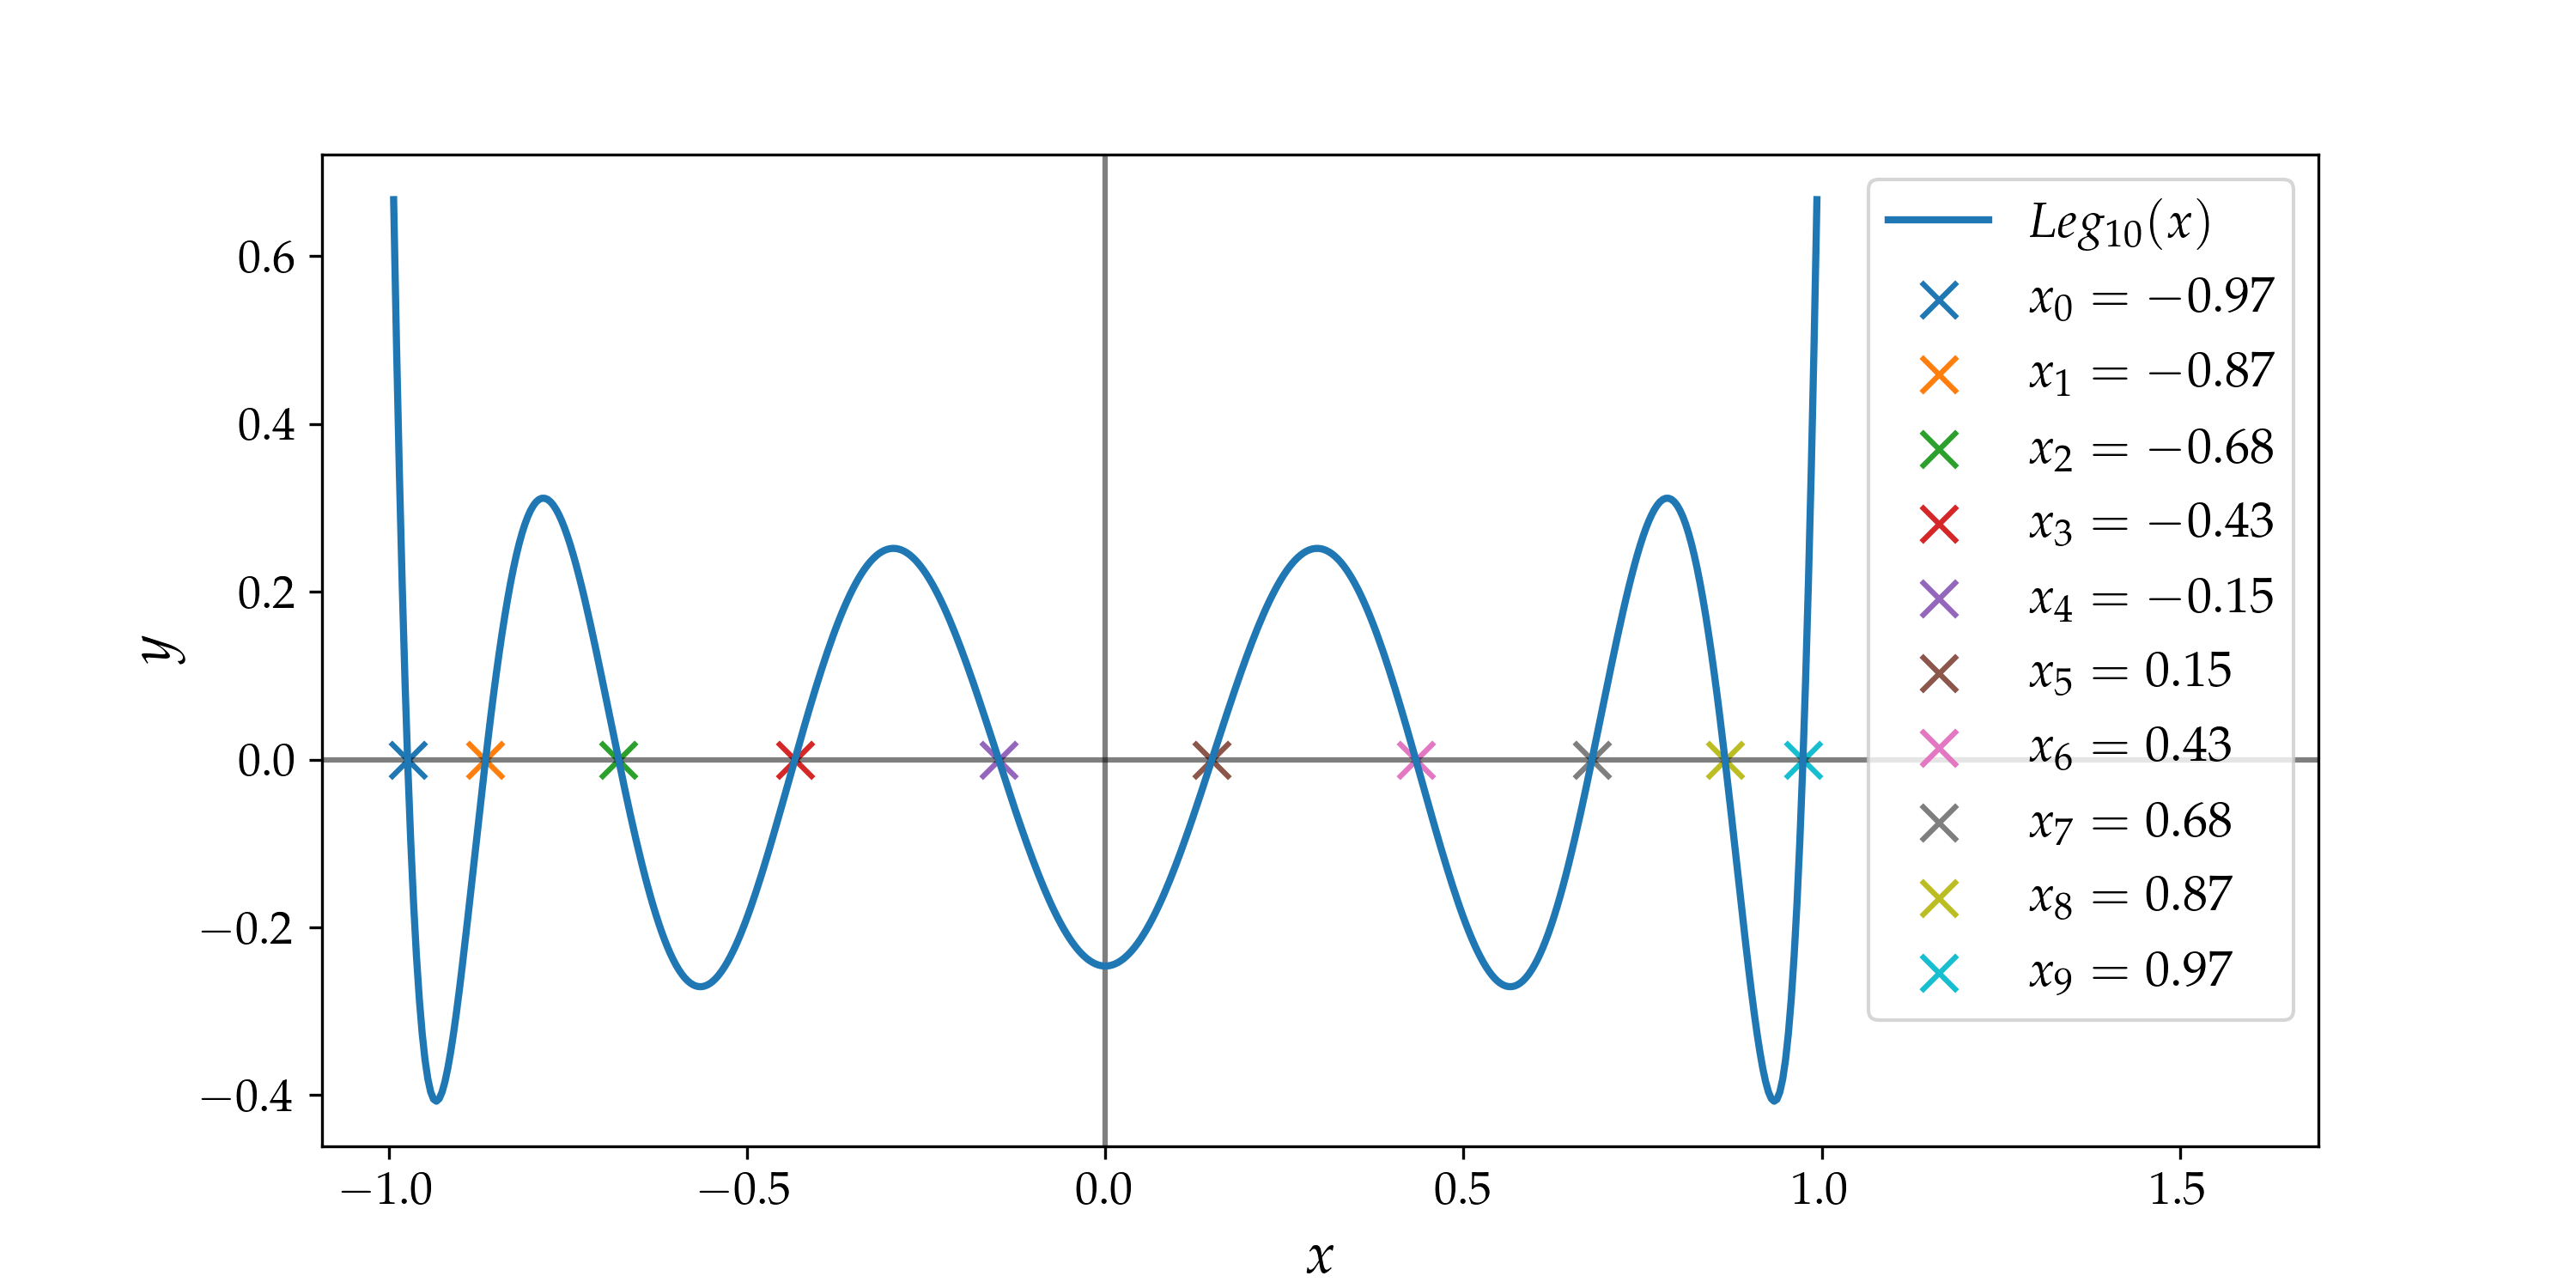
\includegraphics[width=0.8\linewidth]{images/15/Leg_root.png}
    \caption{Il polinomio $\text{Leg}_{10}(x)$, con le relative radici estratte dall'algoritmo.}
    \label{fig: Leg10}
\end{figure}


\subsubsection{Polinomi di Hermite di ordine 6}
Vale un discorso del tutto analogo per $\text{H}_6(x)$: i risultati di seguito.

\begin{elegantcode}
Roots Hermite 6: [-2.35060497 -1.33584907 -0.43607741  0.43607741  1.33584907  2.35060497]

diff_0 = 1.27e-10
diff_1 = 6.08e-12
diff_2 = 4.77e-15
diff_3 = 2.73e-12
diff_4 = 1.28e-11
diff_5 = 2.36e-11
\end{elegantcode}


\begin{figure}[H]
    \centering
    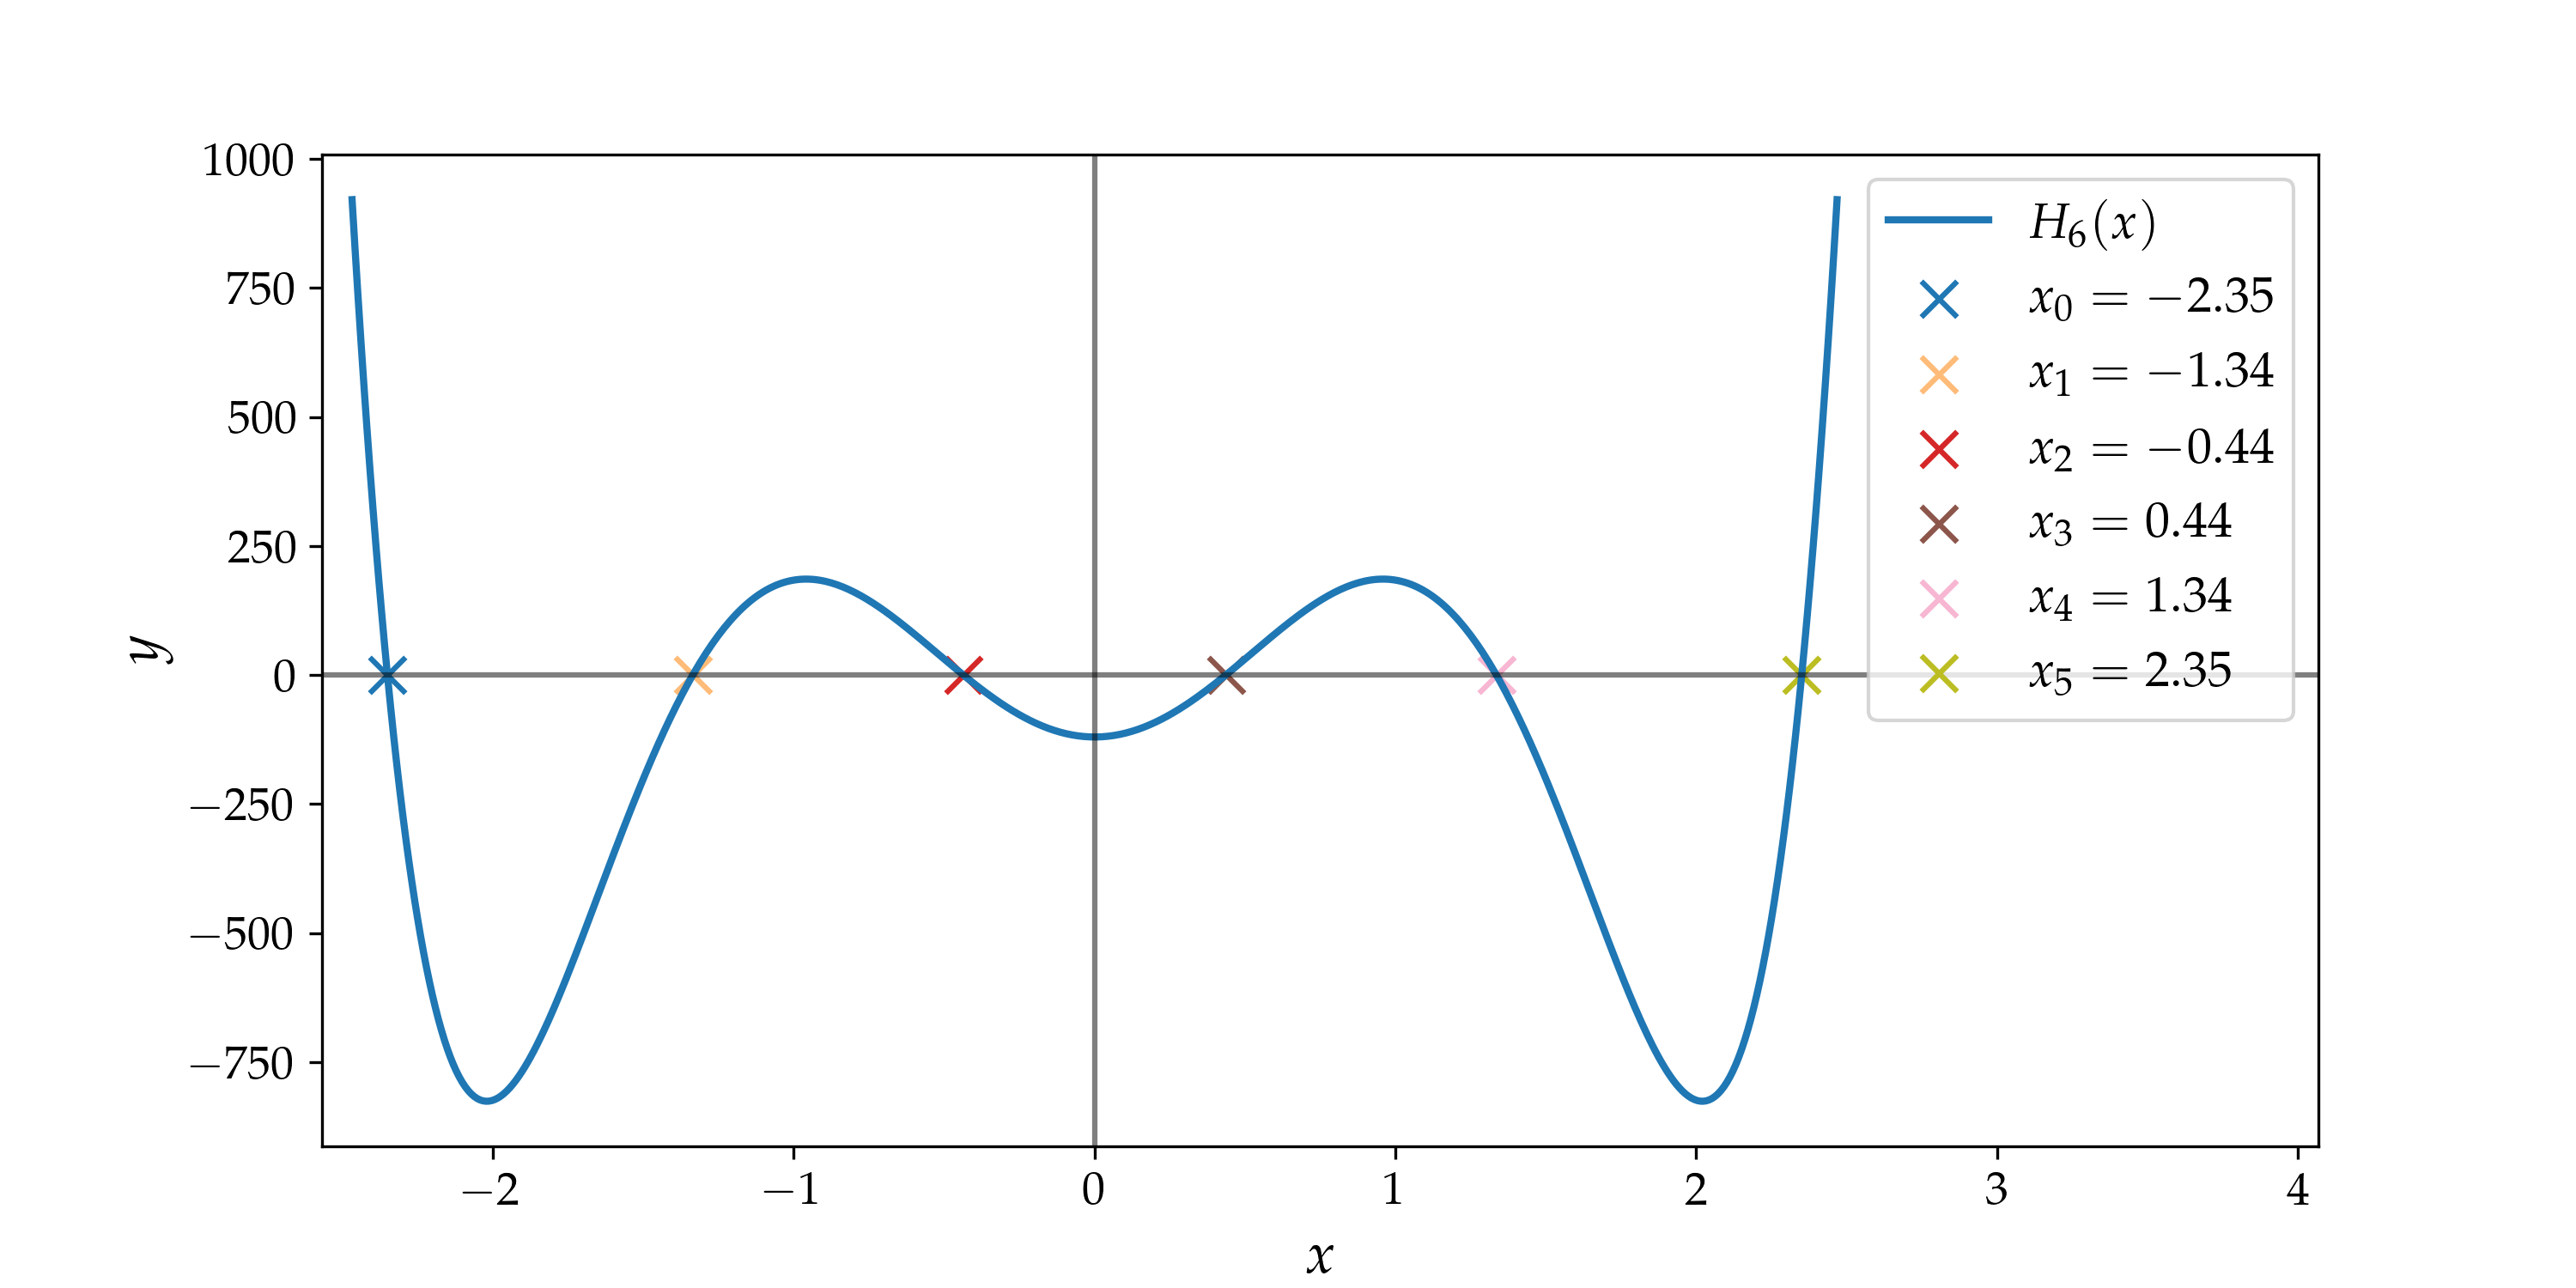
\includegraphics[width=0.8\linewidth]{images/15/Her_root.png}
    \caption{Il polinomio $\text{H}_{6}(x)$, con le relative radici estratte dall'algoritmo.}
    \label{fig: Her6}
\end{figure}


\subsubsection{Polinomi di Hermite di ordine n}
È stato implementato il metodo per il calcolo dei coefficienti del polinomio di Hermite di ordine $n$, che di conseguenza generalizza il caso precedente: siamo quindi interessati a confermare i risultati con un confronto tra i due metodi, che dovrebbero, chiaramente, essere interscambiabili.

\medskip\noindent
In particolare valutiamo la metrica
\[
\delta = \sqrt{\sum_{i=0}^5 (\bar x_i - x_i)^2}
\]
definendo $\bar{\boldsymbol x}$ come il vettore delle radici trovate con il metodo generalizzato.\\
Il risultato numerico è:
\[
\delta = 1.34\times 10^{-13}
\]
Il valore ottenuto è estremamente piccolo ed è compatibile con gli errori numerici accumulati durante il calcolo in precisione doppia.
\newpage





